%%%%%%%%%%%%%%%%%%%%%%%%%%%%%%%%%%%%%%%%%%%%%%%%%%%%%%%%%%%%%%%%%%%%%%%%%%%%%%%%
% Template for ASPLOS papers.
%
% History:
% 
% ASPLOS originally used jpaper.cls for submission but required acmart.cls for the
% final camera-ready version. To avoid a change in format, starting ASPLOS 2024 Fall 
% cycle, both the submission and the camera-ready versions started using acmart.cls.
%
%%%%%%%%%%%%%%%%%%%%%%%%%%%%%%%%%%%%%%%%%%%%%%%%%%%%%%%%%%%%%%%%%%%%%%%%%%%%%%%%%%

% use the base acmart.cls version 1.92
% use the sigplan proceeding template with the default 10 pt fonts
% nonacm option removes ACM related text in the submission. 
\DocumentMetadata{}
\documentclass[nonacm,sigplan]{acmart}

% enable page numbers
\settopmatter{printfolios=true}

% make references clickable 
\usepackage[]{hyperref}
\usepackage[normalem]{ulem}

\usepackage{caption}
% The preceding line is only needed to identify funding in the first footnote. If that is unneeded, please comment it out.
% \usepackage{cite}
% \usepackage{algorithmic}
\usepackage{graphicx}
\usepackage{textcomp}
\usepackage{xcolor}

\usepackage{listings}
\usepackage{booktabs}
\usepackage{multirow}
% \usepackage[linesnumbered,ruled,vlined]{algorithm2e}
% \usepackage{amsmath}
\usepackage{algorithm}
\usepackage{algpseudocode}
\makeatletter
\algrenewcommand\ALG@beginalgorithmic{\small}
\makeatother
\usepackage{enumitem}
\newcommand{\tool}{\textsc{GPUlog}}
\newcommand{\buffer}{Eager Buffer Management }

\newcommand{\kris}[1]{{\textcolor{red}{\{\textbf{Kris}: #1\}}}}
\newcommand{\tom}[1]{{\textcolor{blue}{\{\textbf{Tom}: #1\}}}}
% \newcommand{\yihao}[1]{{\textcolor{orange}{\{\textbf{Yihao}: #1\}}}}
\newcommand{\yihao}[1]{{#1}}
\newcommand{\shovon}[1]{{\textcolor{green}{\{\textbf{Shovon}: #1\}}}}
\newcommand{\newt}[1]{{\textbf{\{Revised: #1\}}}}

% \newcommand{\revised}[1]{{\textcolor{red}{\{\textbf{Revised}: #1\}}}}
\newcommand{\revised}[1]{{#1}}

\begin{document}

\title{Optimizing Datalog for the GPU}

% \author{...} % removed for anonymity
\author{Yihao Sun}
\email{ysun67@syr.edu}
\affiliation{%
  \institution{Syracuse University}
  \city{Syracuse}
  \state{New York}
  \country{USA}
}

\author{Ahmedur Rahman Shovon}
\email{ashov@uic.edu}
\affiliation{%
  \institution{University of Illinois, Chicago}
  \city{Chicago}
  \state{Illinois}
  \country{USA}
}

\author{Thomas Gilray}
\email{thomas.gilray@wsu.edu}
\affiliation{%
  \institution{Washington State University}
  \city{Pullman}
  \state{Washington}
  \country{USA}
}

\author{Sidharth Kumar}
\email{sidharth@uic.edu}
\affiliation{%
  \institution{University of Illinois, Chicago}
  \city{Chicago}
  \state{Illinois}
  \country{USA}
}

\author{Kristopher Micinski}
\email{kkmicins@syr.edu}
\affiliation{%
  \institution{Syracuse University}
  \city{Syracuse}
  \state{New York}
  \country{USA}
}

\begin{abstract}
 Modern Datalog engines (\emph{e}.\emph{g}., LogicBlox, Souffl\'e, \texttt{ddlog}) enable their users to write declarative queries which compute recursive deductions over extensional facts, leaving high-performance operationalization (query planning, semi-na\"ive evaluation, and parallelization) to the engine. Such engines form the backbone of modern high-throughput applications in static analysis, network monitoring, and social-media mining.
 In this paper, we present a methodology for implementing a modern in-memory Datalog engine on data center GPUs, allowing us to achieve significant (up to $45\times$) gains compared to Souffl\'e (a modern CPU-based engine) on context-sensitive points-to analysis of \textsf{httpd}.
 We present \tool{}, a Datalog engine backend that implements iterated relational algebra kernels over a novel range-indexed data structure we call the hash-indexed sorted array (HISA). HISA combines the algorithmic benefits of incremental range-indexed relations with the raw computation throughput of operations over dense data structures. Our experiments show that \tool{} is significantly faster than CPU-based Datalog engines while achieving a favorable memory footprint compared to contemporary GPU-based joins.
\end{abstract}

\maketitle % should come after the abstract
\pagestyle{plain} % should come right after \maketitle



\section{Introduction}
\label{sec:intro}

Declarative languages enable their users to write high-level logical rules that specify acceptable solutions to a problem, leaving efficient implementation to a high-performance backend. In particular, modern CPU-based Datalog engines power state-of-the-art systems in program analysis~\cite{bravenboer2009doop,flores2020ddisasm,balatsouras2016cclyzer,recstep}, social-media mining~\cite{shkapsky2016big,gu2019rasql,socialite, skvortsov2024logica}, and  business analytics~\cite{business-Datalog}. Such engines enable a user to specify deductions (forming an \emph{intensional} database, henceforth IDB) over extensionally manifest relations (the \emph{extensional} database, henceforth EDB). For example, given an input relation \textit{Edge}(\texttt{from},\texttt{to}), the program \textit{REACH} computes
\textit{Edge}'s transitive closure:
\[
\begin{array}{lcl}
    \textit{Reach}(\texttt{from},\texttt{to})  & \!\!\!\! \leftarrow & \!\!  \textit{Edge}(\texttt{from}, \texttt{to}).   \\
    \textit{Reach}(\texttt{from}, \texttt{to}) & \!\!\!\! \leftarrow & \!\! \textit{Edge}(\texttt{from}, \texttt{mid}), \textit{Reach}(\texttt{mid}, \texttt{to}).
\end{array}
\]

The second rule requires recursive computation to a fixed-point: the engine iteratively discovers an ever-larger intensional database (\textit{Reach}), starting from the extensional database (\textit{Edge}).
%The rules run to a fixed-point: the first rule copies \textit{Edge} into \textit{Reach}, and the second rule runs recursively, iteratively discovering incrementally-longer paths. While traditional RDBMS systems support such recursive queries in principle (\emph{e}.\emph{g}., SQL's common table expressions~\cite{Bartholomew2017}), their usage in practice has been limited by their notoriously poor performance and lack of efficient query planning. These performance challenges stem from the substantively different concerns typically faced by large-scale deductive analytics tasks. By contrast, modern Datalog engines employ incrementalized (semi-na\"ive) evaluation, compiling queries into nested loop joins over in-memory, index-organized tables~\cite{indexselection} represented via BTrees~\cite{jordan2019specialized}, tries~\cite{jordan2019brie}, or a similar relation-backing data structure~\cite{byods}. 
%The first rule copies \textit{Edge} into \textit{Reach}, and may be implemented via standard techniques (\emph{e}.\emph{g}., selection in SQL~\cite{sqlguide}). The second rule constitutes the bulk of the computation, and requires iteration to a fixed-point: at each iteration, the engine discovers possibly-new tuples in $\textit{Reach} \bowtie \textit{Edge}$ and merges them into $\textit{Reach}$ until no new reachable edges are found. While traditional RDBMS systems do offer support for recursive queries in principle (\emph{e}.\emph{g}., SQL's common table expressions~\cite{Bartholomew2017}), their usage in practice has been limited by their notoriously poor performance and lack of efficient query planning. These performance challenges stem from the substantively different concerns typically faced by large-scale deductive analytics tasks. Modern engines employ incrementalized (semi-na\"ive) evaluation, compiling queries into nested loop joins over in-memory, index-organized tables~\cite{indexselection} represented via BTrees~\cite{jordan2019specialized}, tries~\cite{jordan2019brie}, or a similar relation-backing data structure~\cite{byods}. 
%In this paper we introduce \tool{}, a GPU-accelerated deductive engine that demonstrates runtime improvements of roughly $10\times$ versus an ideally-configured state-of-the-art CPU-based engine (Souffl\'e) on large deductive-analytic workloads (\emph{e}.\emph{g}., context-sensitive points-to analysis of \texttt{httpd}, see Section~\ref{sec:eval} for our results). \tool{} achieves these results by leveraging a novel SIMD data structure we designed specifically for the implementation of modern Datalogs on the GPU: the hash-indexed sorted array (HISA). Compared to CPU-based representations, HISA enables parallel insertion (which dominates 78\% of Souffl\'e's runtime at 32 threads on transitive closure, see the beginning of this section) and harnesses the massively greater throughput of modern GPUs. Compared to modern GPU-based hash tables (e.g., cuDF, GPUJoin), HISA supports efficient range querying (crucially necessary to avoid asymptotic overhead).
Unfortunately, best-in-class in-memory Datalogs hit scalability walls around $8$--$16$ threads due to the challenges of working with locking, linked data structures in a parallel, shared-memory setting. For example, as we will soon see, when run at $32$ threads on transitive closure, Souffl\'e \cite{jordan2016souffle} (a state-of-the-art CPU-based engine) spends $77.8$\% of its time in serialized tuple deduplication/insertion. 

Compared to CPUs, GPUs offer hundreds of thousands of threads, along with extremely high memory throughput via HBM~\cite{hbm}. However, achieving optimal performance necessitates embracing the GPU's programming model. Traditionally, CPU-based graphics processing code has been accelerated via SIMD instructions (such as AVX and SSE), necessitating that all threads operate in lockstep and strongly penalizing thread divergence. While GPUs are inspired by this SIMD paradigm, modern GPGPU programming is SIMT in nature, allowing parallel execution at a per-thread granularity. Threads can diverge at the sub-warp level using advanced thread scheduling techniques~\cite{simt}.
As we will see, the SIMT nature of modern GPUs is a natural fit for Datalog, which stresses both massive data parallelism (\emph{e}.\emph{g}., large joins), \emph{and} task parallelism (\emph{e}.\emph{g}., multiple rules).

% By contrast, GPUs have \yihao{hundreds} thousands of threads and AL; clearly, CPU-based approaches will not suffice to enable scalable Datalog on the GPU.
% The crux of the matter is that Datalog's dense loop is range-indexed joins: unlike in SQL (where indices may not be known a-priori), Datalog engines ensure each relation is indexed so that it may always be efficiently range-queried rather than iterated.

% Modern GPUs provide thousands of parallel data threads in their high-throughput SIMD design, making them well-suited for implementing high-performance Datalog engines. Implementing Datalog requires executing key relational algebra operations like join, union, and projection, along with tasks like sorting and merging buffers \emph{iteratively}. Most prior work has focused on optimizing these tasks in isolation via batch processing. Performing these tasks iteratively and scalably while accounting for the SIMD architecture and restrictive memory patterns of GPUs presents challenges. In this work, we introduce \tool{}, a GPU-accelerated Datalog engine that achieves roughly 10x runtime speedups versus an optimally configured state-of-the-art CPU engine (Souffl\'e) on large deductive-analytic workloads (\emph{e}.\emph{g}., context-sensitive points-to analysis of \texttt{httpd}, see Section~\ref{sec:eval} for our results).

In this paper, we introduce \tool{}: a GPU-based library for parallel relational algebra kernels, enabling the execution of Datalog programs on modern GPUs. \tool{} is backed by a novel SIMT data structure: the hash-indexed sorted array (HISA). We designed HISA to balance the concerns of modern Datalog on the GPU, enabling three critical tasks: (1) efficient range queries, necessary for joins, (2) lock-free deduplication, and (3) parallel iteration. Additionally, \tool{} provides abstractions for optimized evaluation of $n$-way loop-joins we call \emph{temporarily-materialized} joins, offering a space-for-time trade-off we found crucial to scale to high data loads.

%Modern GPUs offer (tens of) thousands of data threads of computation in their high-throughput SIMD architecture, making them an ideal target for implementing high-performing deductive engines. Implementing Datalog requires performing key relational algebra operations such as join, union, and projection and other tasks such as sorting and merging buffers in a loop. Most existing work has been limited to optimizing these tasks in a standalone manner where they are executed in batch mode. Performing these tasks \emph{iteratively} in a scalable manner while dealing with the SIMD hardware architecture and restrictive memory access patterns (contiguous) of the GPU is a challenging task. In this paper, we introduce \tool{}, a GPU-accelerated deductive engine that demonstrates runtime improvements of roughly $10\times$ versus an ideally-configured state-of-the-art CPU-based engine (Souffl\'e) on large deductive-analytic workloads (\emph{e}.\emph{g}., context-sensitive points-to analysis of \texttt{httpd}, see Section~\ref{sec:eval} for our results).

%The optimal performance of \tool{} can be attributed to several algorithmic innovations, at the heart of which is our novel SIMD data structure the hash-indexed sorted array (HISA), which we designed specifically for the implementation of modern Datalogs on the GPU. HISA harnesses the massively greater throughput of modern GPUs, crucially enabling three tasks: (1) efficient range queries, necessary to perform joins (2) fast deduplication, necessary to perform RA operations in a loop, and (3) parallel insertions (which dominates 78\% of Souffl\'e's runtime at 32 threads on transitive closure, see the beginning of this section). Compared to modern GPU-based hash tables (e.g., cuDF, GPUJoin), HISA supports efficient range querying (crucially necessary to avoid asymptotic overhead).
%\tool{} achieves these results by leveraging a novel SIMD data structure we designed specifically for the implementation of modern Datalogs on the GPU: the hash-indexed sorted array (HISA). Compared to CPU-based representations, HISA enables parallel insertion (which dominates 78\% of Souffl\'e's runtime at 32 threads on transitive closure, see the beginning of this section) and harnesses the massively greater throughput of modern GPUs. Compared to modern GPU-based hash tables (e.g., cuDF, GPUJoin), HISA supports efficient range querying (crucially necessary to avoid asymptotic overhead).
%Implementing Datalog requires performing a series of joins, also known as $n$-way joins. While most existing work focuses only on 2-way or binary joins, \tool{} presents an efficient implementation of the generalized $n$-way join. We achieve an $$n$-way$ join by breaking it down into a series of $(n-1)$ binary joins, where the results of each binary join are fully materialized (temporarily stored) to be used as input for the next binary join. This implementation is well-suited to GPU architecture since it maximizes data parallelism and locality. In addition to temporary materialized joins, we have introduced an effective space-for-time trade-off technique that is especially beneficial for systems with high VRAM capacity.
%performing temporal materialization of the result of binary joins materializing the output of every binary join prepari
%involve more than two relations at every iteration of the fixed-point loop.  Performing  Most existing work focuses on binary joins involving only two relations. We enabling 
%While using HISA, we also implement two key algorithmic innovations: (1) eager buffer management, and (2) temporal materialization of joins. With eager buff
%To optimize \tool{} for the specific hardware architecture and contiguous memory access patterns of GPUs, computation-intensive operations such as iterative joins, sorting, and merging are implemented in a two-phase fashion. Initially, this involves estimating the computational workload and preparing an appropriately sized, contiguous result buffer. Subsequently, the computation results are efficiently collated and integrated into this buffer. Additionally, we have introduced an effective space-for-time trade-off technique, particularly beneficial for systems with high VRAM capacity. 

We have used \tool{} to implement and comprehensively study the performance of graph analytics (reachability, same generation) and program analysis (points-to analysis), evaluating \tool{} against cuDF, GPUJoin, and Souffl\'e \cite{cudf, shovon2023towards, jordan2016souffle}. We observe improved ($5\times$) join performance compared to state-of-the-art GPU join algorithms (due to efficient range queries enabled by HISA), along with significantly reduced memory footprint. Additionally, \tool{} is the first-ever GPU Datalog implementation to achieve net-positive performance versus CPU-based engines, beating Souffl\'e (a leading CPU-based solver) by up to $45\times$ (NVIDIA H100 \tool{} vs. EPYC 7543P Souffl\'e). Our contributions are as follows:
\begin{itemize}
%\item A systematization of the key differences and necessities of in-memory Datalog engines in the SIMD/GPU vs. shared-memory/CPU setting.
\item The Hash-Indexed Sorted Array (HISA), a novel relation-backing data structure which provides range querying while leveraging the efficiencies of dense representations.

\item \tool{}, a CUDA-based library for implementing Datalog queries on the GPU; \tool{} uses HISA as its tuple representation. \tool{} also leverages two novel strategies apropos Datalog on the GPU: eager buffer management and temporarily-materialized $n$-way joins. 

\item A thorough evaluation of \tool{}, and a performance comparison between \tool{} and state-of-the-art CPU and GPU-based Datalog engines and GPU joins; we show \tool{} outperforms prior work by $5$--$45\times$ with favorable memory footprint.

% \item An evaluation of \tool{} which evaluates its performance as a high-throughput SIMD hash table.

% \item An evaluation of our eager buffer management strategy, showing that it significantly improves buffer allocation.

% \item An evaluation comparing \tool{} to both CPU and GPU-based systems for deductive-analytic queries, showing that \tool{} outperforms every system against we evaluate (often by a significant factor). 
%Next , we discuss how we use HISA to implement \tool{}, 

\end{itemize}

%We begin by surveying the design and implementation of modern CPU-based deductive database systems, particularly remarking upon their scalability 
%bottlenecks. We next shift to discussing concerns regarding a relation-backing SIMD data structure for iterated joins on the GPU, before introducing our solution (the HISA) in Section~\ref{sec:impl-data}. Section~\ref{sec:gdlog} then discusses how we leverage HISA to build \tool{}. Our evaluation is in Section~\ref{sec:eval}, after which we conclude.

\section{Datalog and Declarative Analytics}
\label{sec:datalog}


Datalog has yielded exciting results for a diverse set of data-heavy analytic applications such as static program analysis~\cite{bravenboer2009strictly}, graph mining~\cite{seo2013socialite}, and machine learning~\cite{
mooney1996inductive}. Its growing popularity lies in its expressive and elegant semantics for specifying computations. Datalog programs comprise an extensional database (EDB) of explicit facts and an intensional database (IDB) of derived facts, transitively inferred from the rules and EDB~\cite{green2013datalog}. The language's rules, written as Horn clauses, define relationships between data, and Datalog operates by iteratively applying these rules until no more knowledge is discovered~\cite{maier2018datalog}. Each rule consists of a head and a body. The general form of a Datalog rule is:
\[
\begin{array}{lcl}
 \textit{Head}(...)  & \leftarrow & \textit{Body}_1(...), ..., \textit{Body}_n(...).
\end{array}
\]
The head, represented by a single predicate atom, signifies the derived fact to be inferred. The body, made up of comma-separated predicate atoms, specifies the conditions for the head's truth, with commas serving as a logical "AND" ($\land$). 
The implication symbol $\leftarrow$ connects the head and body, signaling that the head is derived when the body's conditions are met. This structure is closely related to concepts in relational database management systems (RDBMS). Notably, the sharing of logical variables across body clauses directly corresponds to a \emph{join} operation on the related columns in an RDBMS. However, Datalog's foundation in logic programming transcends the capabilities of traditional SQL. It leverages this foundation to unlock greater expressive power, enabling functionalities like recursion and inference beyond simple data retrieval~\cite{10.1145/2892208.2892226}.

% For instance, consider the second rule of the REACH query introduced in beginning of section \ref{sec:intro}. Here, the ``mid'' variable, shared between clauses, indicates a join between the second column of the \textit{Edge} table and the first column of the \textit{Reach} table. The results of this join, following the logic of all body clauses, are then inserted into the table associated with the head clause. 


\paragraph*{Semi-na\"ive evaluation}
Modern Datalog engines owe their algorithmic benefits to incremental evaluation techniques such as semi-na\"ive evaluation~\cite{abiteboul1995foundations}, differential/timely dataflow~\cite{Naiad, mcsherry2013differential}, and DBSP~\cite{dbsp}. Following Souffl\'e, \tool{} uses semi-na\"ive evaluation, which builds a \emph{frontier} of freshly-discovered facts, avoiding the inevitable re-discovery of a fact at every subsequent iteration. To illustrate this process, consider the Same Generation (\emph{SG}) query, used to determine if two nodes in a graph share a topological order:
\[
\begin{array}{lcl}
    \textit{SG}(\texttt{x},\texttt{y}) & \leftarrow & \textit{Edge}(\texttt{p},\texttt{x}), ~ \textit{Edge}(\texttt{p}, \texttt{y}), ~ \texttt{x} \neq \texttt{y}. \\
    \textit{SG}(\texttt{x}, \texttt{y}) & \leftarrow & \textit{Edge}(\texttt{a}, \texttt{x}), ~ \textit{SG}(\texttt{a},\texttt{b}), ~ \textit{Edge}(\texttt{b},\texttt{y}), \texttt{x} \neq \texttt{y}.
\end{array}
\]
% Here, the \textit{Edge} relation stores all edges within the input graph. When nodes $x$ and $y$ are determined to be of the same generation (implying a shared topological ordering) an \textit{Edge} $(x, y)$ fact will be established in the database. 
In this query, \textit{Edge} represents extensional edges in the input graph. The first rule states that nodes \texttt{x} and \texttt{y} are in the same generation if they have a common parent node \texttt{p}. The second rule recursively derives \textit{SG} by determining that \texttt{x} and \texttt{y} are in the same generation if there exists a node \texttt{a} with an outgoing edge to \texttt{x}, and another node \texttt{b} with an outgoing edge to \texttt{y}, such that \texttt{a} and \texttt{b} are themselves in the same generation.

The semi-na\"ive evaluation strategy optimizes this query execution, by maintaining the \textit{SG} relation in three versions: ``\textit{new}'' (containing tuples generated in the current iteration), ``\textit{delta}'' (holding unique tuples added in the previous iteration), and ``\textit{full}'' (comprising all tuples derived across all iterations). By performing the join operation solely on the \textit{delta} relation, the engine significantly reduces redundant computation.
% leading to substantial performance gains over na\"ive evaluation strategies.
% We visualize this strategy by Figure~\ref{fig:sg-iter1} and Figure~\ref{fig:sg-iter2}.

\begin{figure}
    \centering
    % 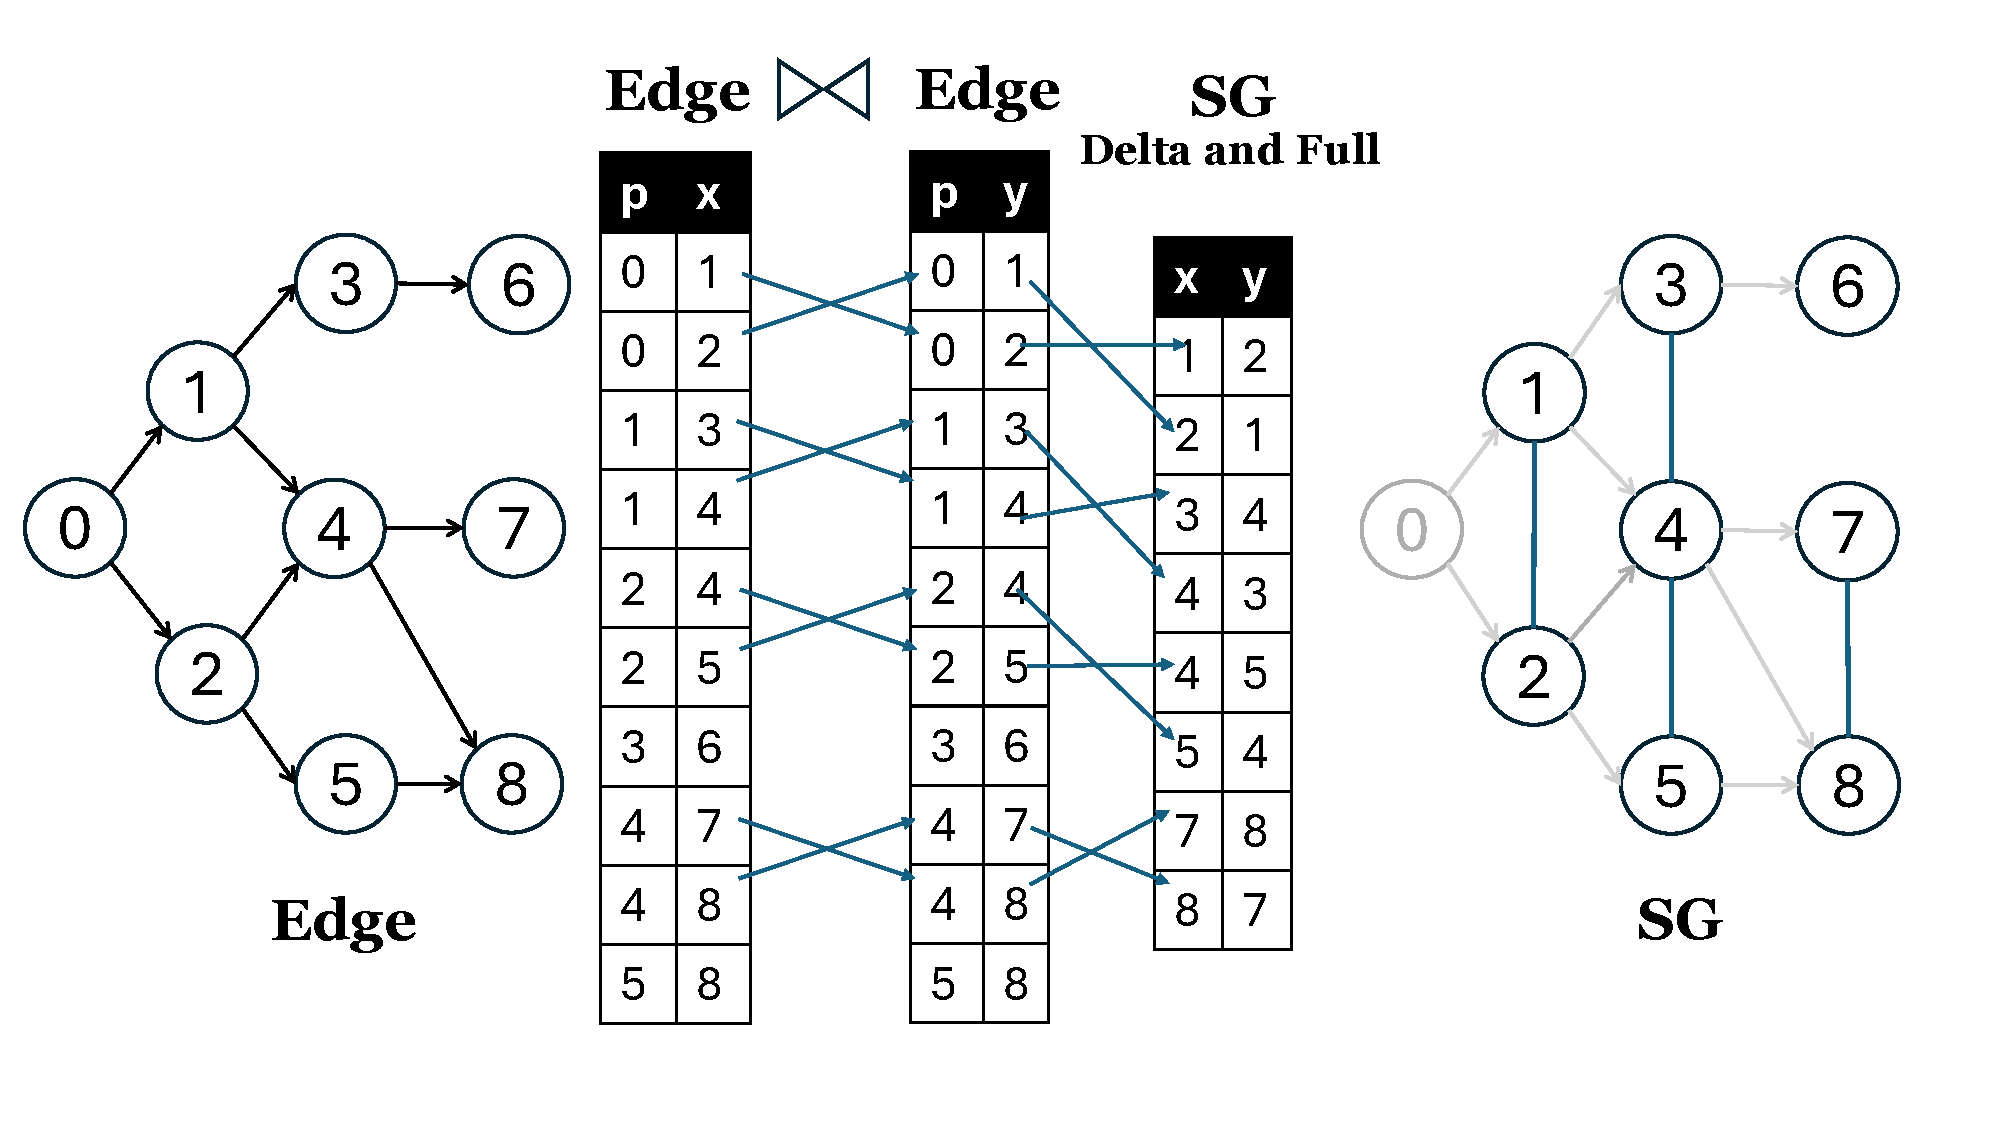
\includegraphics[width=\linewidth]{figures/sg_iter1.pdf}
    % 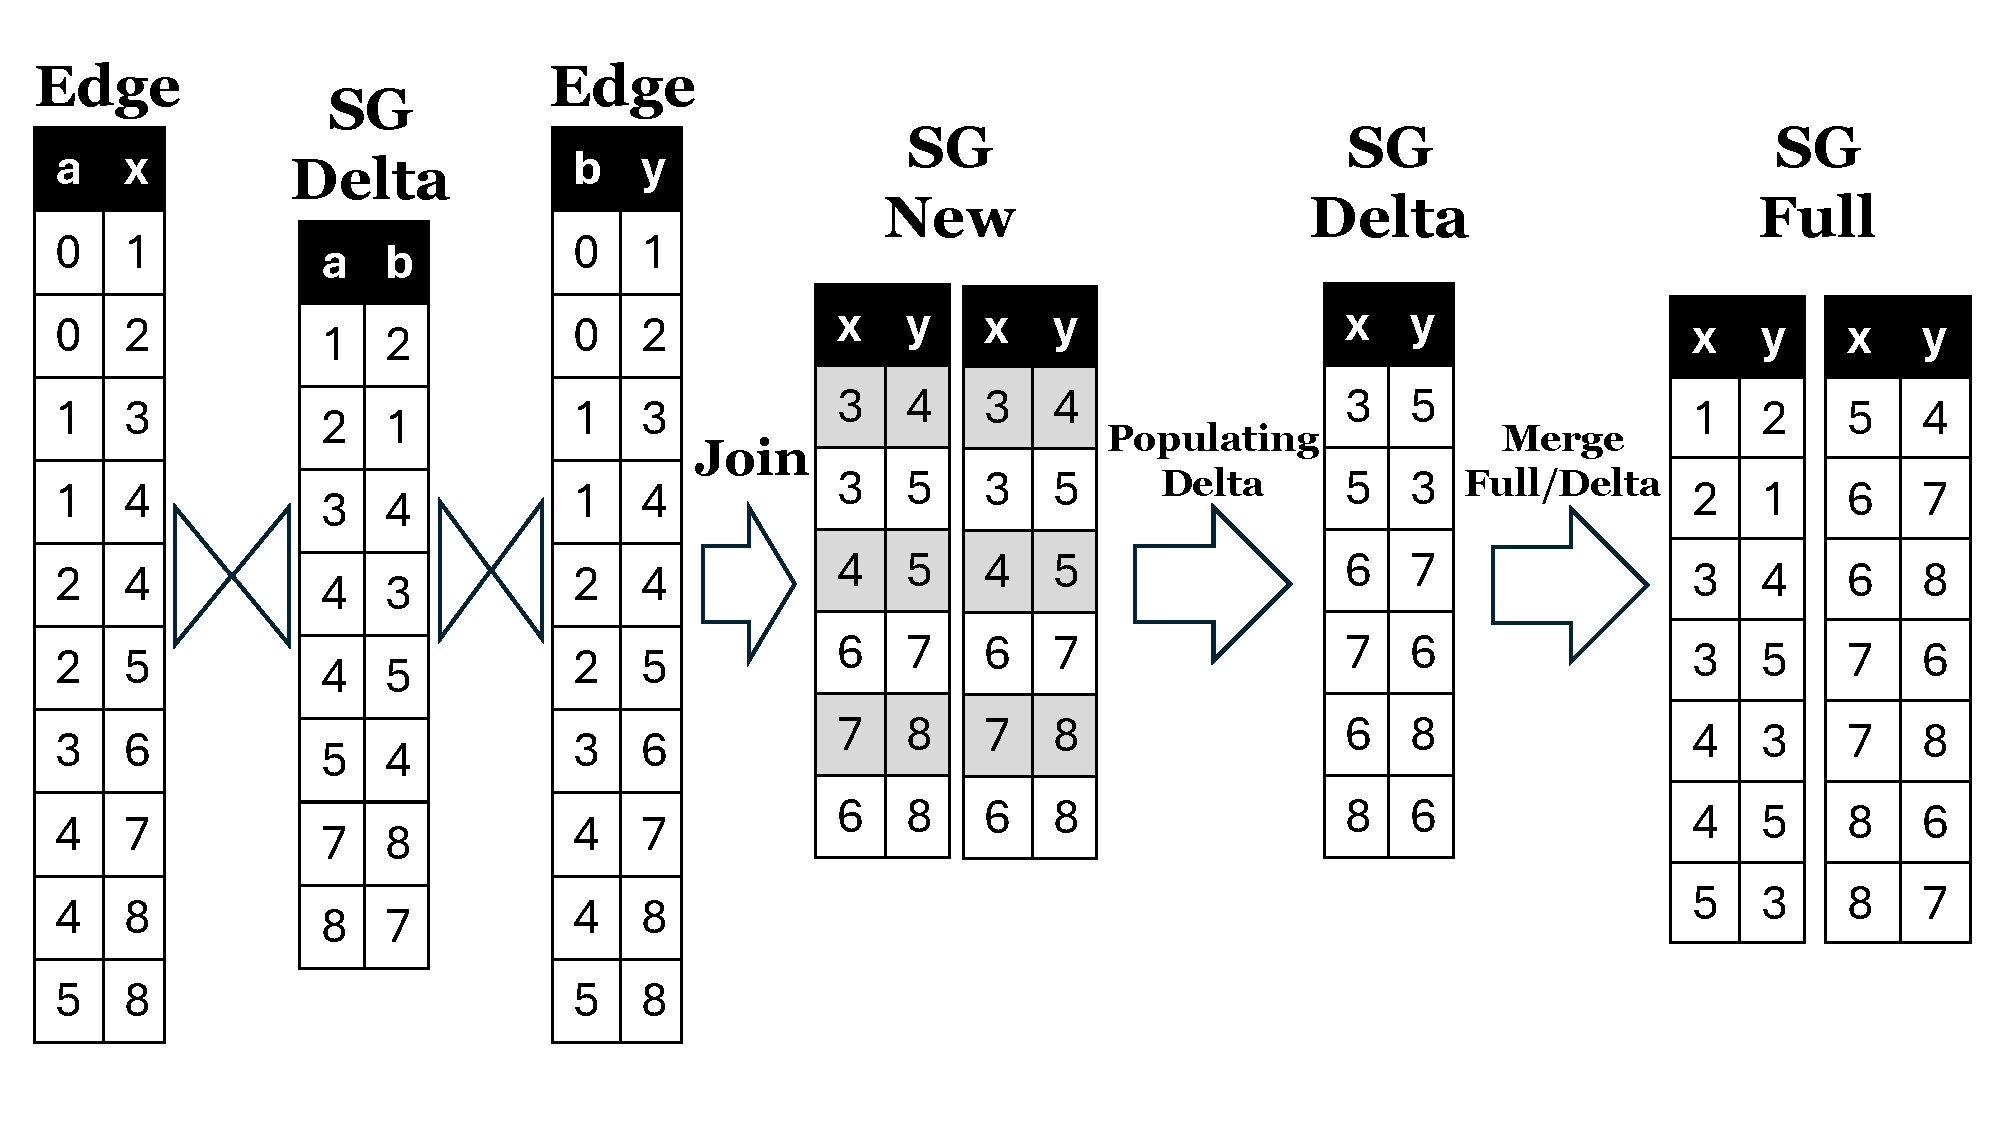
\includegraphics[width=\linewidth]{figures/sg_iter2.pdf}
    % 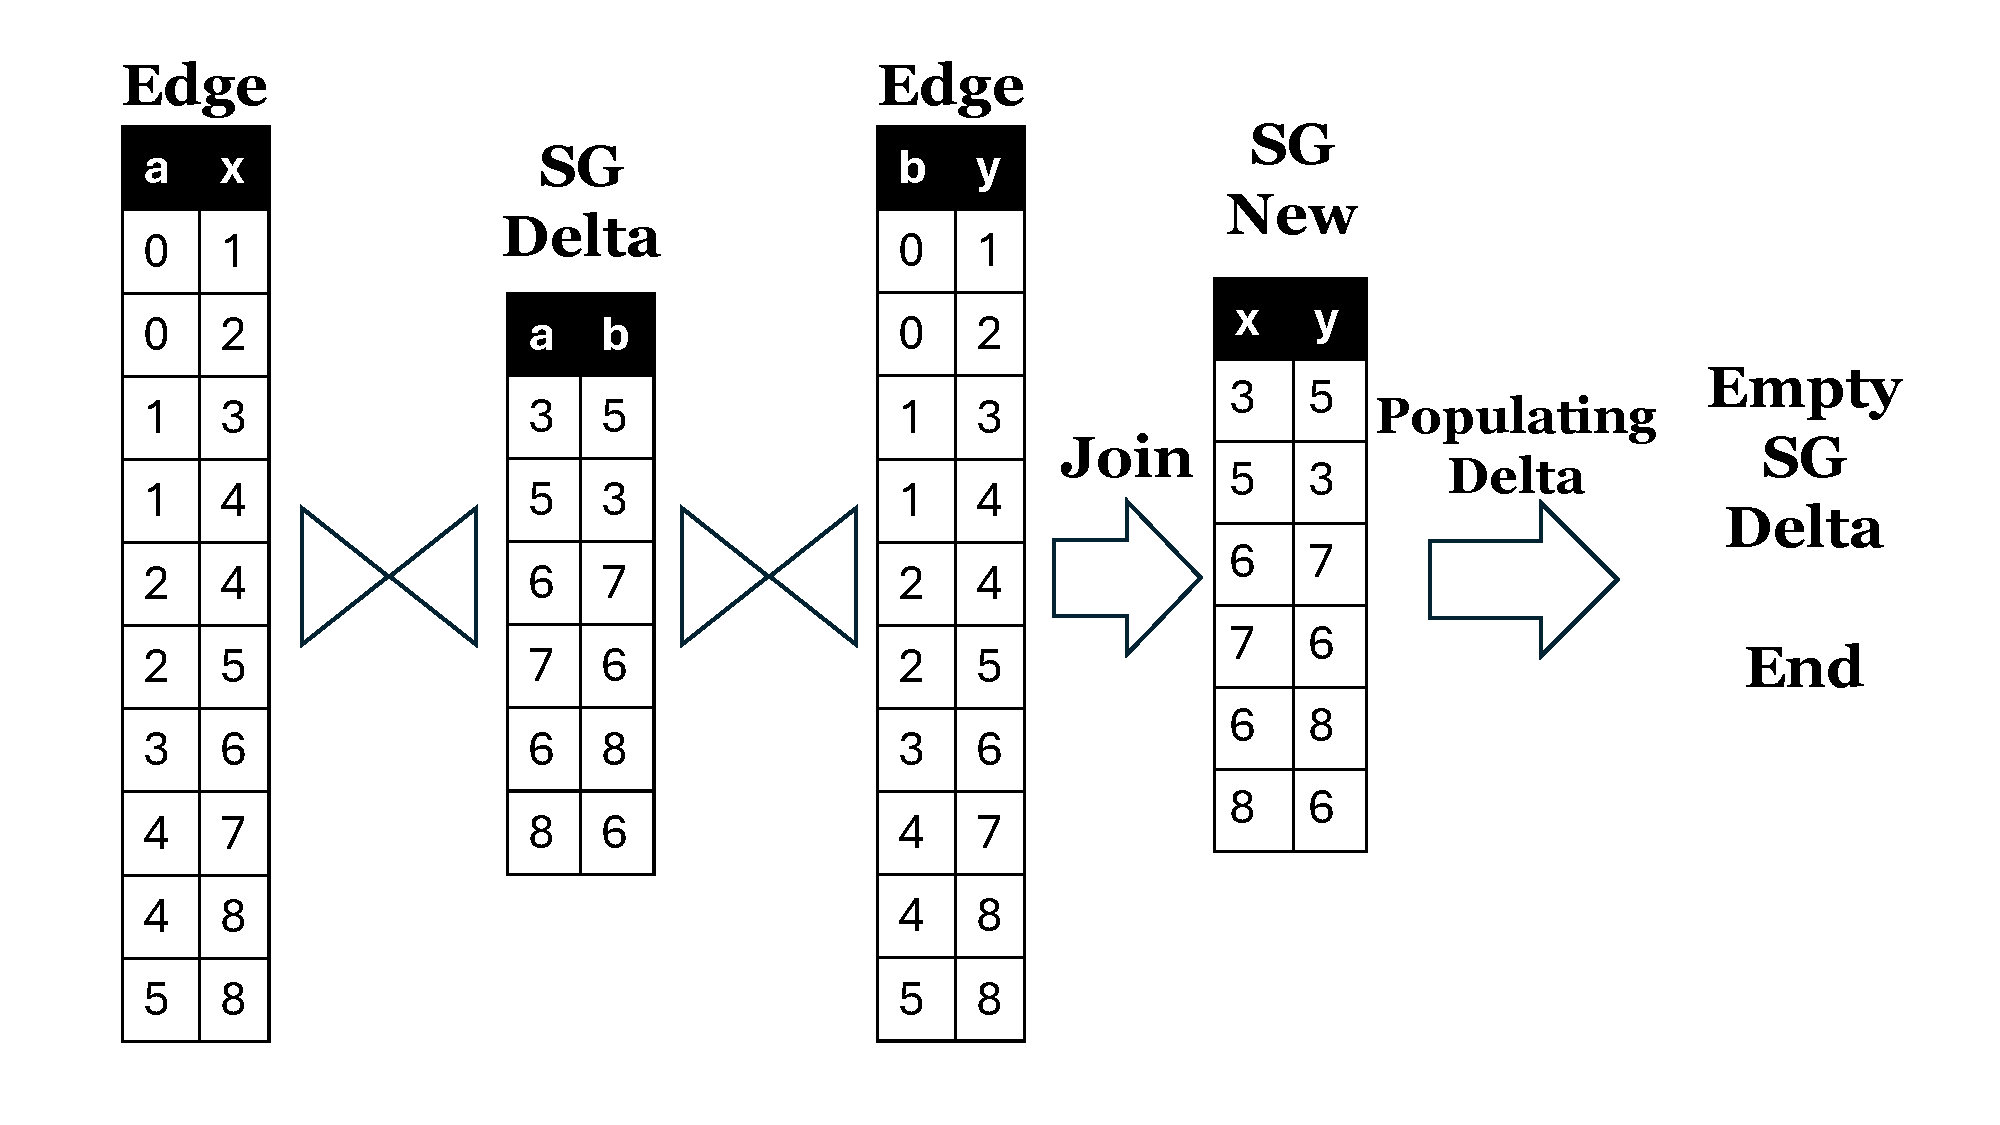
\includegraphics[width=\linewidth]{figures/sg_iter3.pdf}
    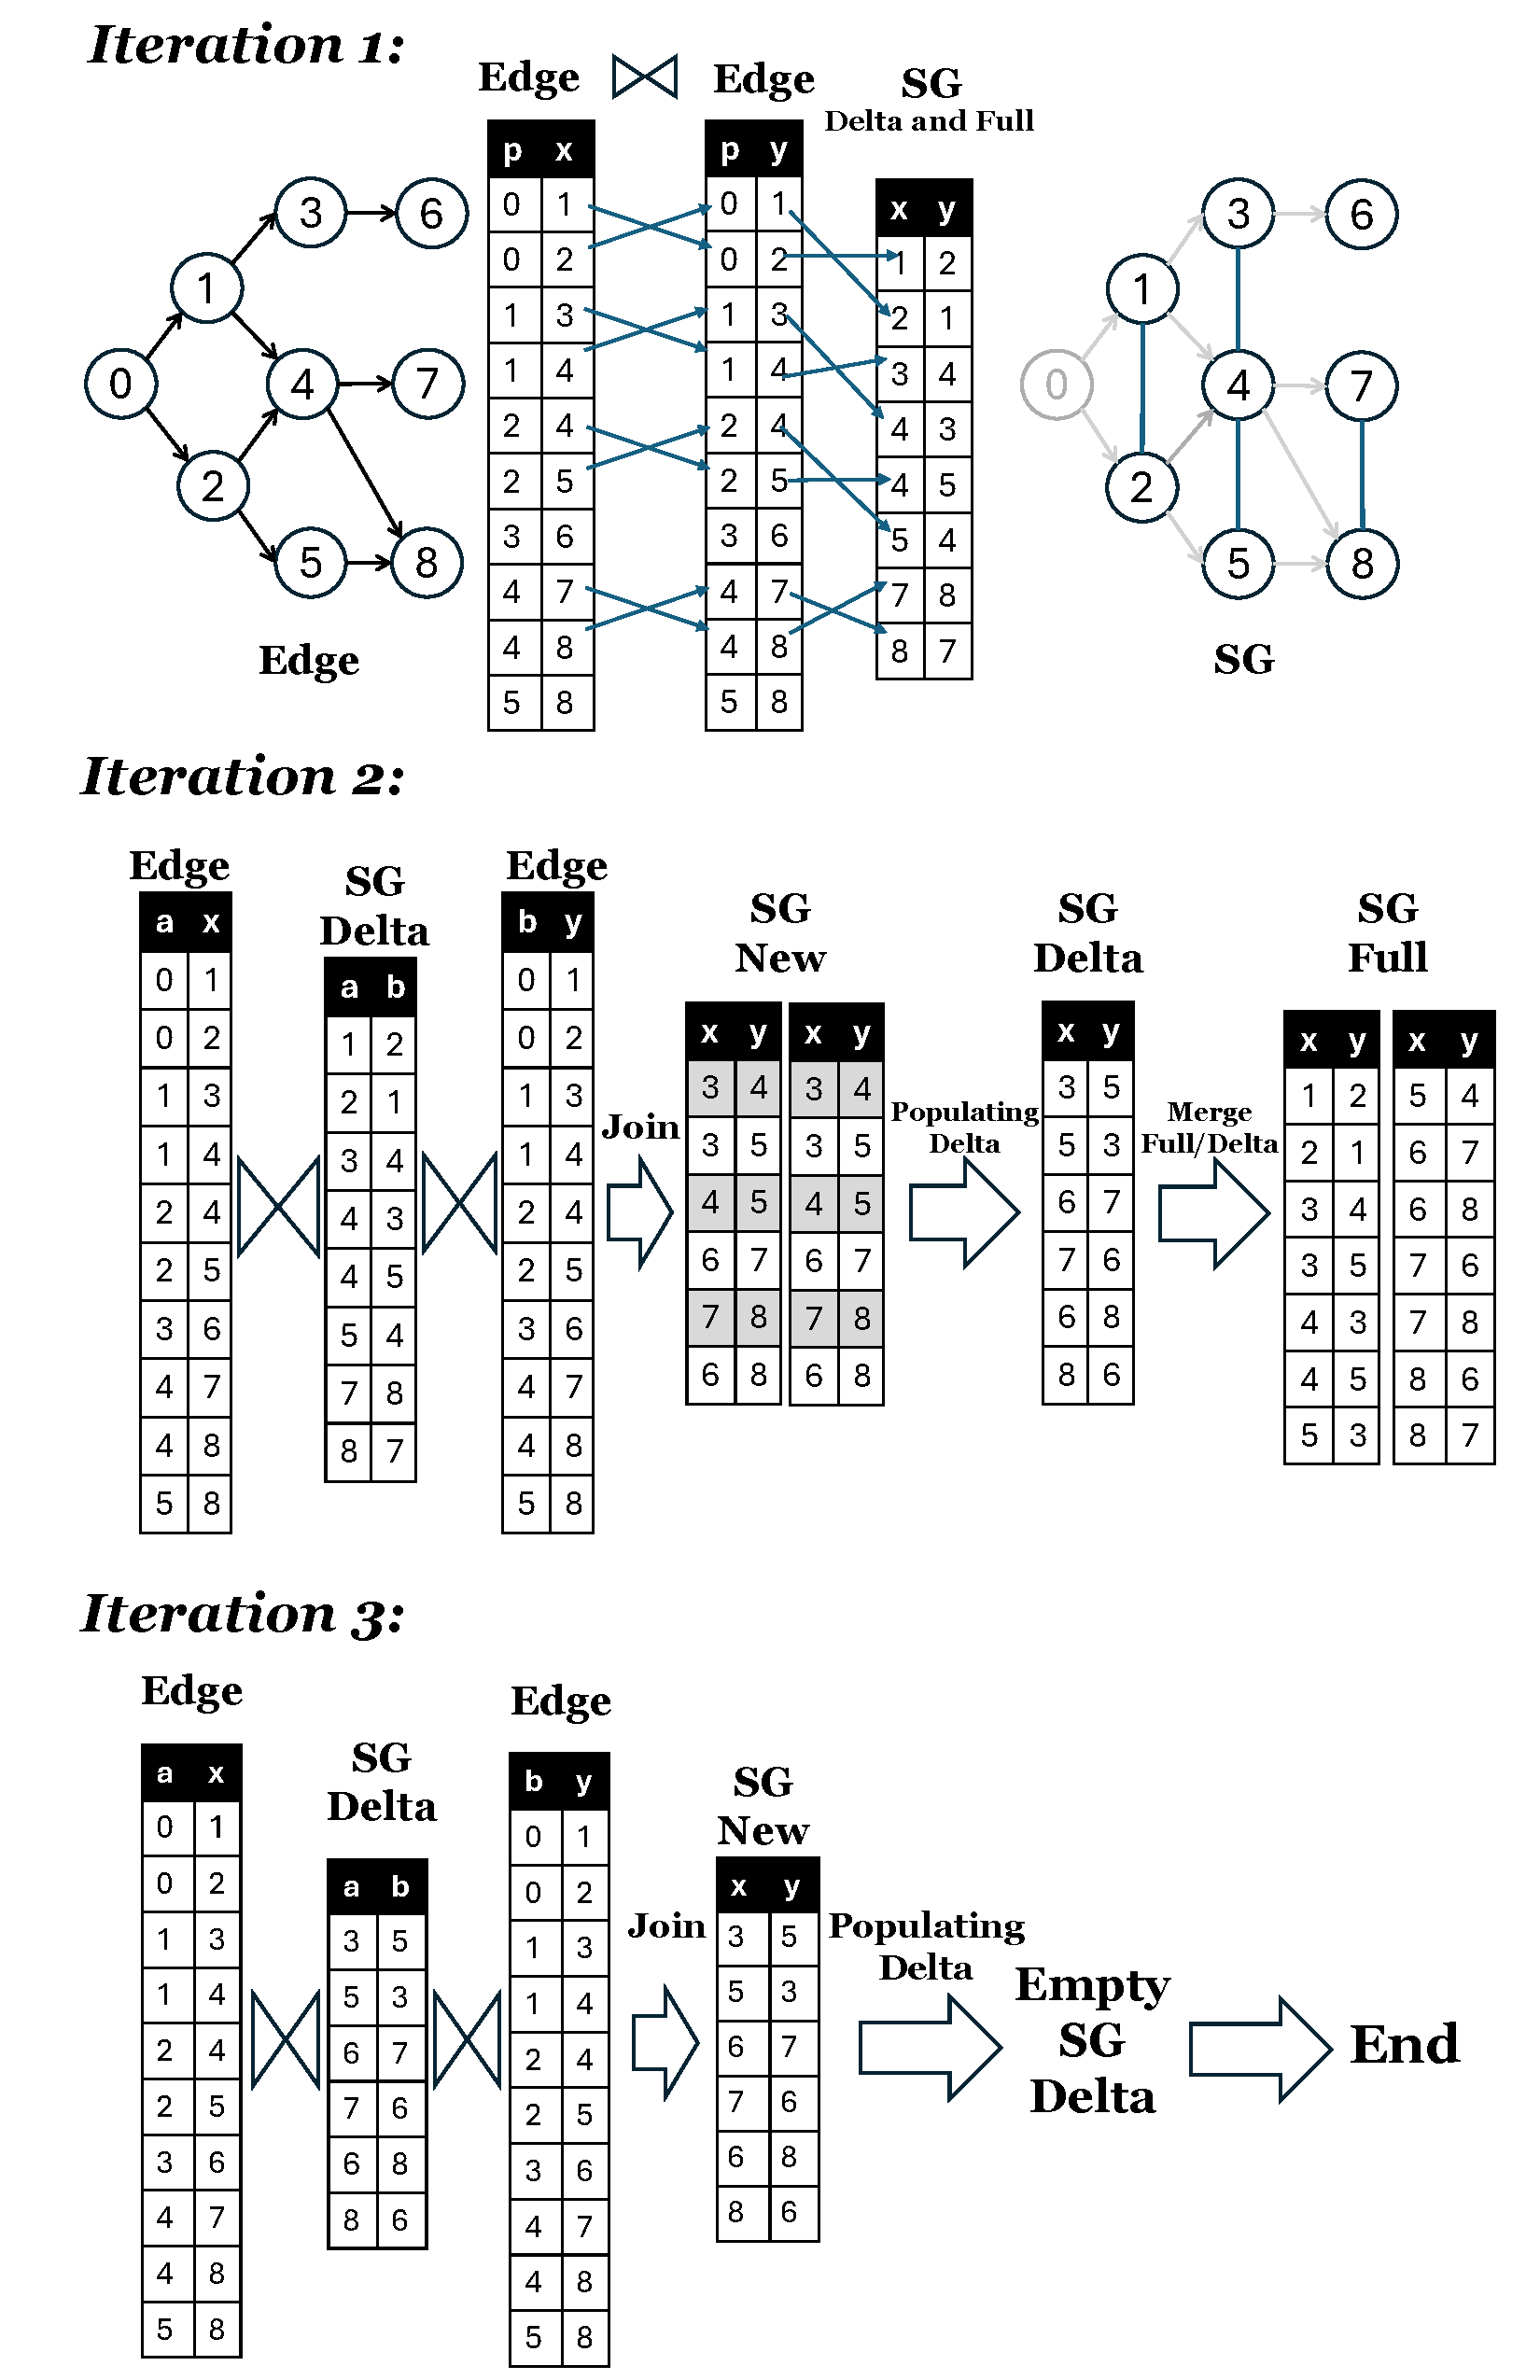
\includegraphics[width=\linewidth]{figures/combined_sg.pdf}
    \caption{\fontsize{9}{11}\selectfont The execution results of each iteration in Same Generation (SG) query.}
    \label{fig:sg-iter}
    % \vspace{-0.5cm}
\end{figure}

\paragraph*{Example} Figure~\ref{fig:sg-iter} illustrates each iteration of the \textit{SG} query. During the first iteration, only the first rule generates new tuples since \textit{SG} is empty and thus the second rule yields nothing.
This rule applies when two edges in the graph merge from the same starting node but lead to different destination nodes; these edges are joined to generate new \textit{SG} tuples. For instance, the tuple $\textit{SG}(7,8)$ is produced by joining $\textit{Edge}(4,7)$ and $\textit{Edge}(4,8)$, both of which originate from node $4$. Upon completing the first iteration, the newly generated tuples are moved into both the \textit{delta} and \textit{full} versions of the \texttt{SG} relation, preparing them for subsequent computation.

% \begin{figure}
%     \centering
%     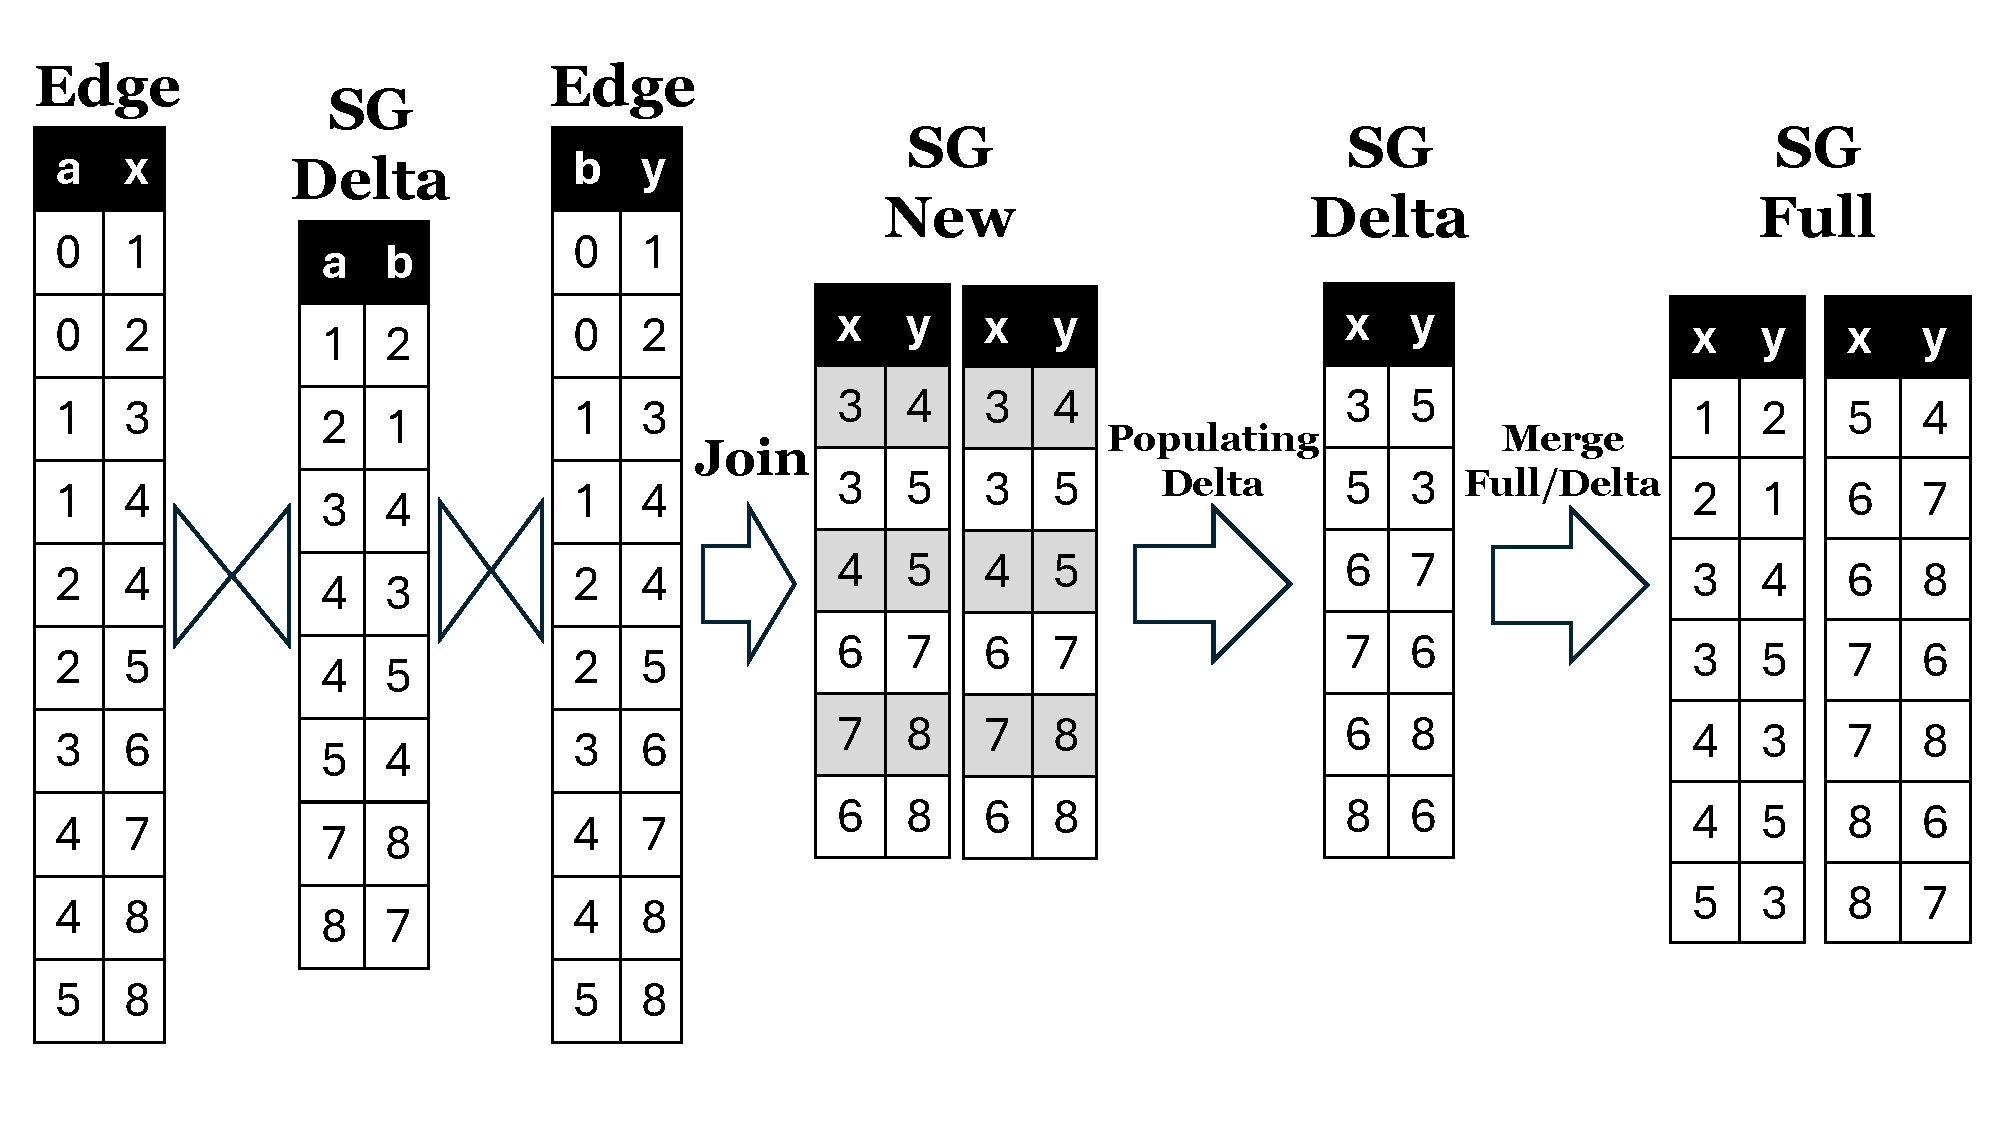
\includegraphics[width=\linewidth]{figures/sg_iter2.pdf}
%     \caption{The join and deduplication operation in the $2^{nd}$ of the Same Generation Query. The grey rows in $\textit{SG}_{new}$ are duplicates.}
%     \label{fig:sg-iter2}
% \end{figure}
%Since, at the end of the first iteration, the relation $SG$ gets populated delta where the SG relation's inductive cases are engaged.
The middle of Figure~\ref{fig:sg-iter} shows the second iteration involving a three-way join: $\textit{Edge} \bowtie \textit{SG}_{delta} \bowtie \textit{Edge}$, leading to the derivation of indirect same generation tuples, such as $\textit{SG}(6,8)$, from $\textit{Edge}(3,6)$, $\textit{Edge}(4,8)$, and $\textit{SG}(3,4)$ (in the \textit{delta} version). Notice that the \textit{new} version of the \texttt{SG} relation, generated post-join, contains duplicates tuples from its \textit{full} version, such as $\textit{SG}(3,5)$ and $\textit{SG}(7,8)$.
To ensure maintain the invariant that \textit{delta} and \textit{full} are disjoint, a deduplication process is implemented both within the \textit{delta} and against the \textit{full} set as the \textit{new} tuples are allocated. 


% \begin{figure}
%     \centering
%     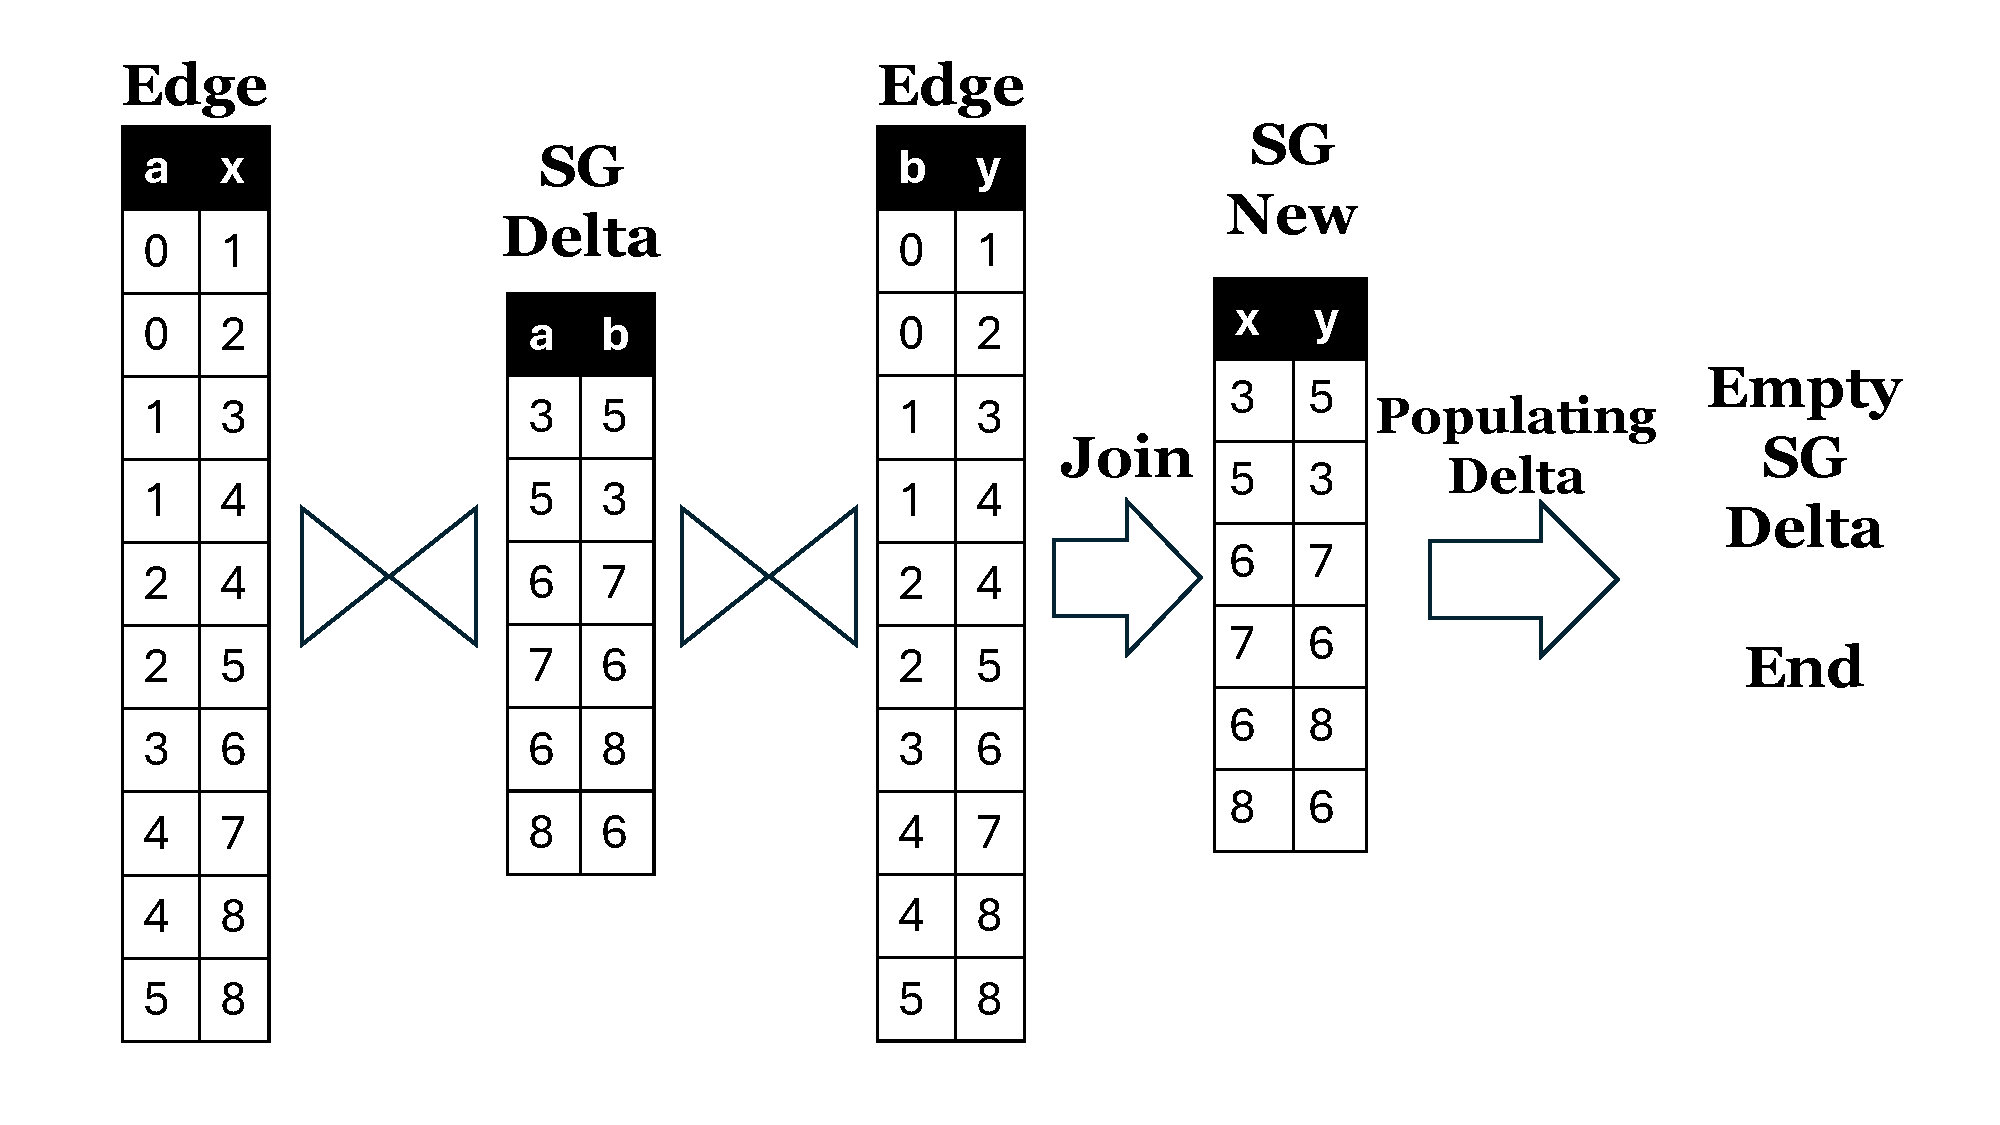
\includegraphics[width=\linewidth]{figures/sg_iter3.pdf}
%     \caption{The join and deduplication operation in the $2^{nd}$ of the Same Generation Query.}
%     \label{fig:sg-iter3}
% \end{figure}

% \kris{yihao: edit plz, then remove this comment.}
After completing the second iteration, the Datalog engine proceeds with the third iteration, as shown in the bottom of Figure~\ref{fig:sg-iter}. The previous iteration's $\textit{SG}_\textit{delta}$ is used as the input for the join operations in the current iteration. The join results in new tuples $\textit{SG}_{new}$; however, all of these tuples are already present in $\textit{SG}_{full}$, leading to an empty $\textit{SG}_{delta}$. This indicates that the query has reached its fixpoint.  We revisit semi-na\"ive evaluation in more detail within the context of our GPU-based implementation in Section~\ref{sec:impl-data}.

% Note, in our \emph{Same Generation} query implementation, the \emph{non-recursive} first rule is executed only once (first iteration), as determined by the query planner. While query plan creation is crucial for executing Datalog, our work focuses on implementing the generated plans. For our experiments, we manually generate query plans for small Datalog programs and use Souffl\'e for larger ones.



%It is important to note that in our implementation for the SG query, the first rule is not reevaluated in the second and third iterations. This is because the first rule is non-recursive, and consequently, the query planner, responsible for computing join plans, marks it to be executed only once. While creating the query plan is a crucial part of the end-to-end pipeline for executing Datalog, our work primarily focuses on the implementation of the generated query plans. For all the experiments presented in this paper, we either manually generate the query plan for smaller Datalog programs or rely on Souffle for larger Datalog programs.



%these tuples are already present  Following the deduplication phase in this iteration, no \textit{new} tuples are added to \textit{delta}, indicating that the query has reached its fixpoint. 
% The final result of the query is stored in the current \textit{full} version of \texttt{SG}.




% \begin{figure}
%     \centering
%     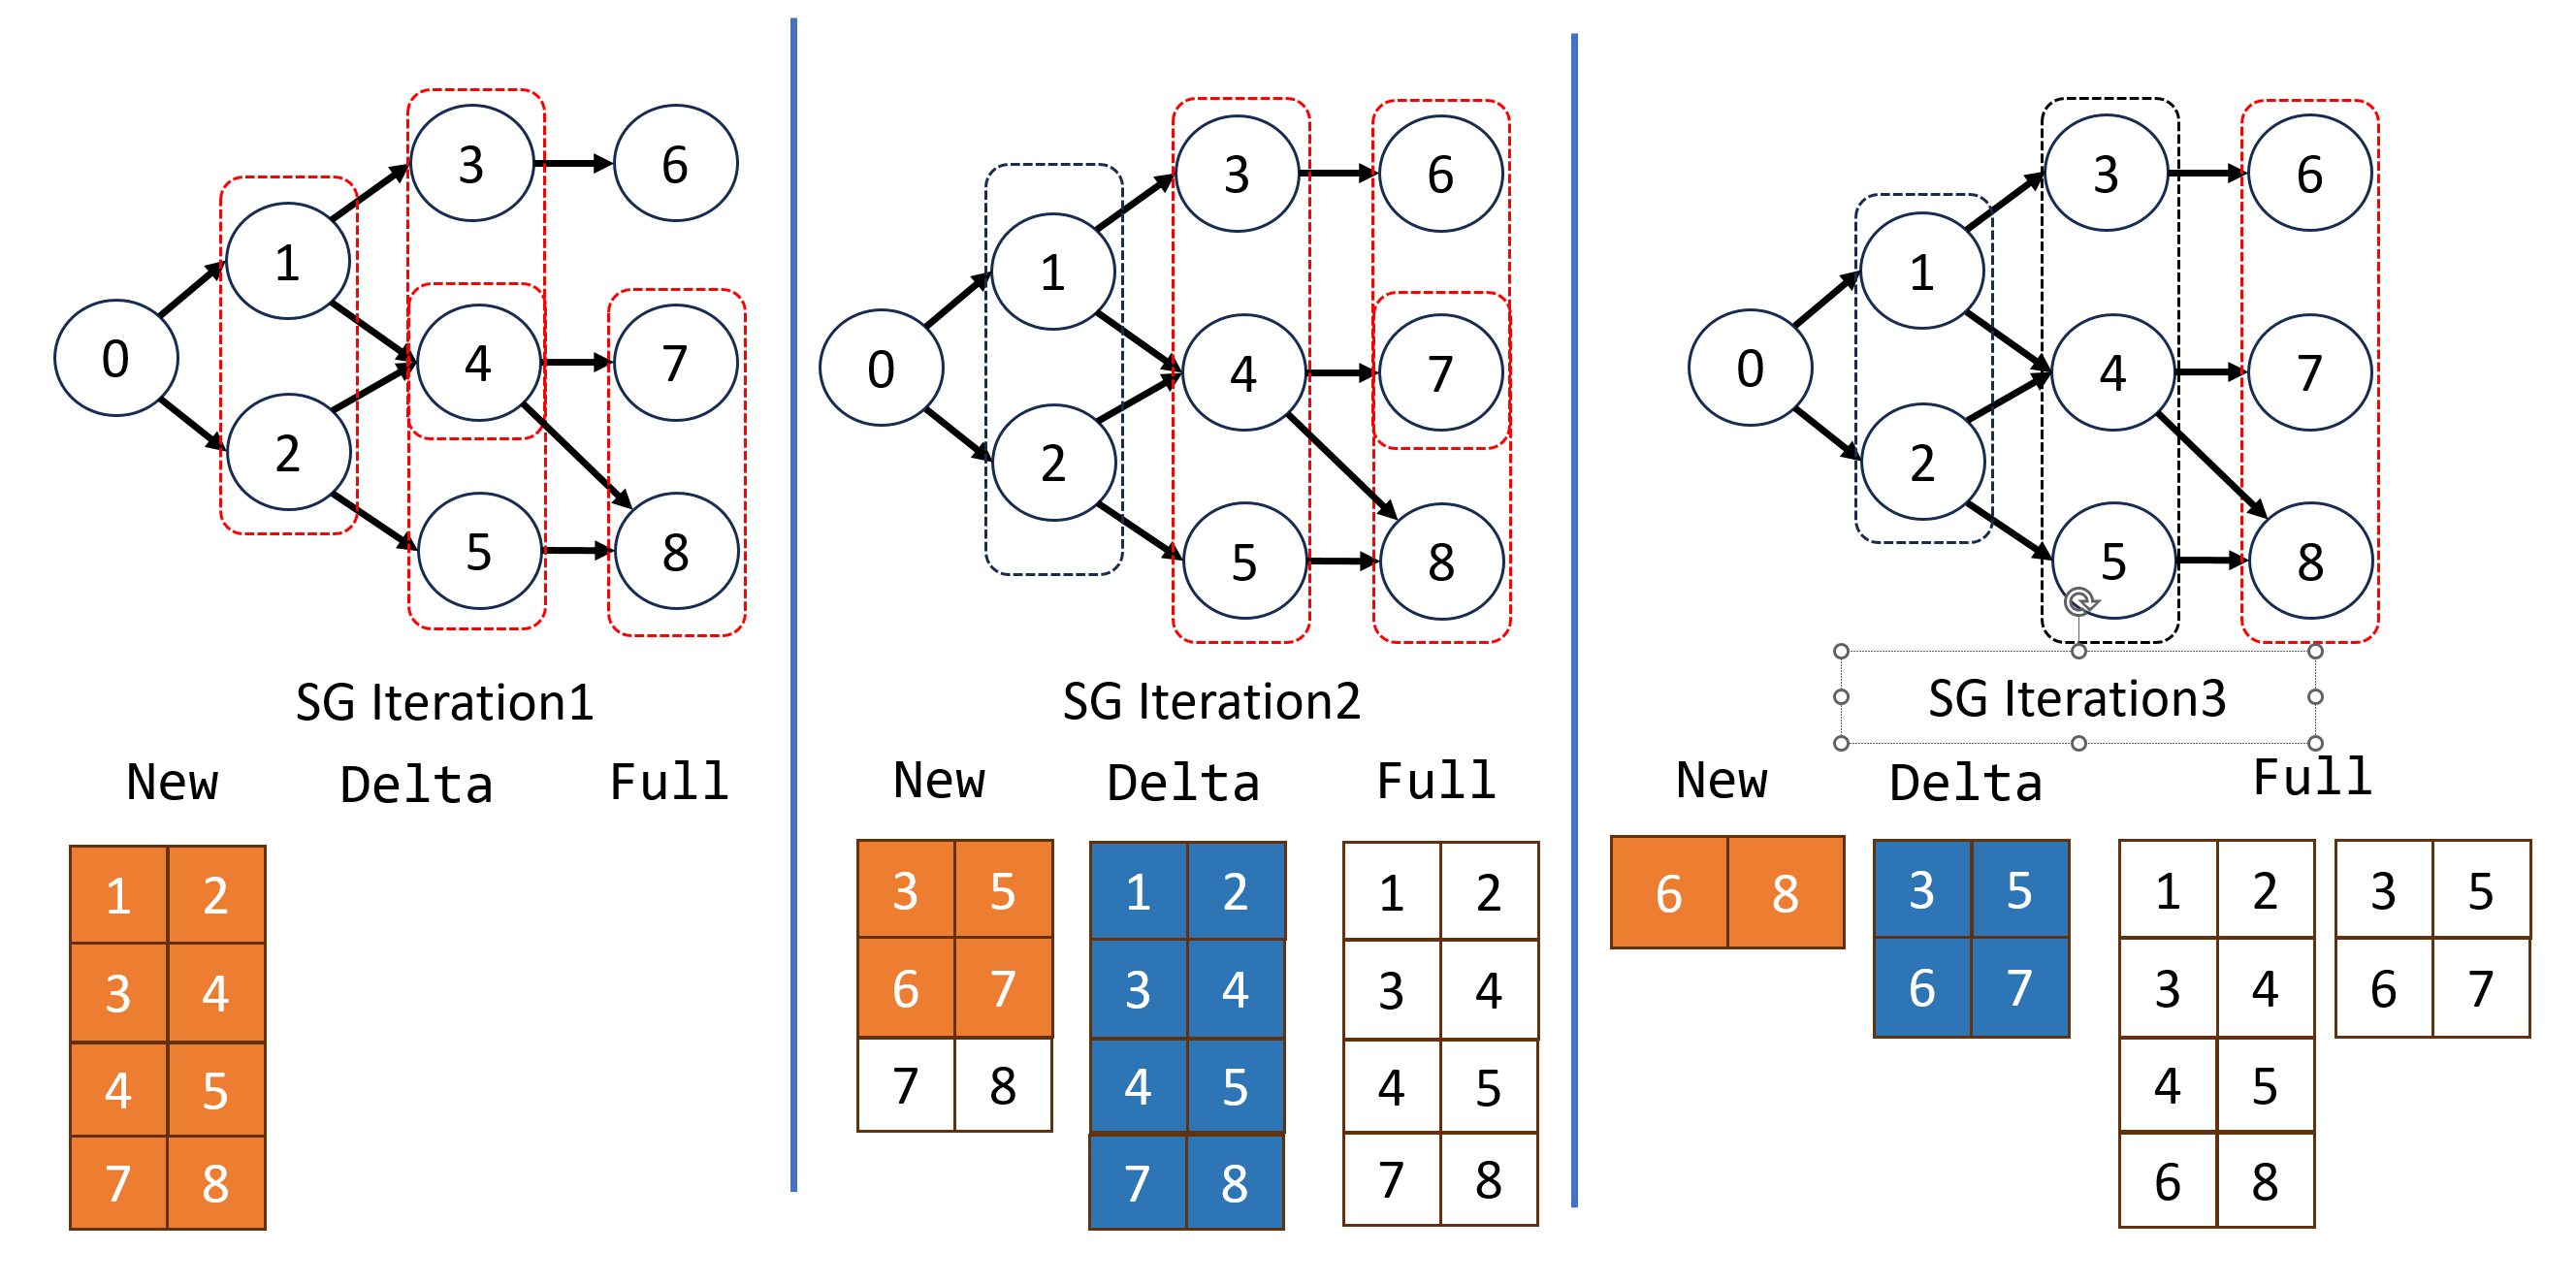
\includegraphics[width=\linewidth]{figures/sg_explain.png}
%     \caption{Evaluation of Same Generation(SG) query using semi-na\"ive evaluation}
%     \label{fig:sg-explain}
% \end{figure}

% The detail of semi-na\"ive evaluation is visualized in Figure \ref{fig:sg-explain}.  Within the first iteration, the first rule is used to populate the SG tuples where the identical edges emerge from the same preceding nodes. For example, considering the tuple $\texttt{SG}(7,8)$, which results from the join of $\texttt{Edge}(4,7)$ and $\texttt{Edge}(4,8)$.  As a result, the tuples $\texttt{SG}(1,2)$, $\texttt{SG}(3,4)$, $\texttt{SG}(4,5)$, and $\texttt{SG}(7,8)$ deriving from the corresponding Edge tuples, are then inserted into the \textit{new} version of the SG.  Preparing for subsequent iterations, Datalog engine clears out the \textit{delta} version. Tuples from the \textit{new} version are simultaneously migrated to both the \textit{full} and \textit{delta} version of SG, and then the \textit{new} version is emptied. Consequently, at the beginning of iteration two, the \textit{delta} version is refreshed with tuples discovered during the first iteration. 

% During the second iteration, the engine activates the second rule of the SG query. This rule recursively derives new SG tuples based on the existing SG tuples from the previous iteration. 
% For example, the tuple $\texttt{SG(7, 8)}$ is derived from $\texttt{Edge(4,7)}$,  $\texttt{SG(4,5)}$ (present in the \textit{delta} version), and $\texttt{Edge(5,8)}$. The tuple $\texttt{SG}(7,8)$ then stored in \textit{new} version of SG. It is critical to highlight the deduplication step of semi-na\"ive evaluation: it ensures that tuples already present in the \textit{full} version, like $\texttt{SG}(7,8)$, are not redundantly computed or moved again into the \textit{full} and \textit{delta} versions. This deduplication prevents unnecessary work in subsequent iterations.

% The process described is iteratively repeated by the Datalog engine until no additional tuples are added to the \textit{delta} version during an iteration. In the example illustrated in the figure, a fixpoint is reached after the conclusion of the third iteration, and the \textit{full} relation at this times is the final result of the query.



\section{GPU Datalog: Challenges and Concerns}
\label{sec:motivation}

%\kris{inner and outer is no longer defined}

The high performance of modern Datalog engines (such as Souffl\'e~\cite{jordan2016souffle} and BigDatalog~\cite{shkapsky2016big}) is due to a combination of factors, including compilation, data structures, and semi-na\"ive evaluation. Among these, we focus on the design of a GPU-based relation-backing data structure. In the context of relevant related work, we outline four key requirements demanded of a GPU-based relation-backing data structure. No state-of-the-art implementations sufficiently satisfy all of our requirements (at least, in a fully-general manner).

% upon which relational algebra operations are implemented. 

%We now outline four key requirements demanded of a GPU-based relation-backing data structure for implementing Datalog on the GPU.

% Datalog is ultimately operationalized into relational algebra kernels involving operations such as joins, projections, and union on relations. Implementing these kernels on the GPU requires relation-backing data structures for storing tuples (Section~\ref{sec:relationDS}) and requires handling multi-way joins (Section~\ref{sec:impl-k-way}).
% %operations that can support fast range-queries  as we .... These kernels are executed iteratively in a fixed point loop till no new facts/tuples can be discovered. 
% In this section, we detail the challenges in implementing Datalog on GPUs.
%will outline the implementation challenges for modern Datalog engines, particularly those based on GPU architecture.

%Modern implementations typically perform range-indexing on relations to enable indexed nested loop joins. To better understand the data structure requirements, let's examine the join operation in more detail. Algorithm \ref{alg:join} provides a generalized description of a join. It involves a for-loop that iterates over each tuple in one of the relations, referred to as the outer relation. Within this loop, for each tuple of the outer relation, a range query fetches all tuples from the inner relation, filtering to include only tuples  with matching values in the joined columns.

% \begin{algorithm}
% \caption{Datalog Relational Join Process}
% \begin{algorithmic}[1]
% \For{$t_{o}$ in $Relation_{outer}$}
%     \State $jc \gets$ join\_columns $\in t_{o}$
%     \State $matched \gets$ $Relation_{inner}.$range($jc$)
%     \For{ $t_{i}$ in $matched$}
%         \State Compute result from $t_{o}$ and $t_{i}$
%     \EndFor
% \EndFor
% \end{algorithmic}
% \label{alg:join}
% \end{algorithm}

\paragraph*{[R1]: Efficient Range-Querying} Joins $R(\ldots) \bowtie Q(\ldots)$ are  operationalized in modern Datalog engines via loop-joins, scanning $R$ and range-querying $Q$, or mutatis mutandis for $Q$ and $R$. 
To support range-querying, tuples are organized (\emph{e}.\emph{g}., via indexing) to associate sets of tuples with a set of join columns. We call the scanned relation the \emph{outer} relation, and the range-indexed relation the \emph{inner} relation. Compared to traditional RDBMS systems---which cannot possibly compute optimal indices due to the ad-hoc nature of querying---modern Datalog engines perform indexing for \emph{every} query~\cite{indexselection}.
Modern engines employ a mix of minimally-locking linked data structures such as B-trees and Bries \cite{jordan2019specialized,jordan2019brie,byods}, and are carefully tuned for optimal performance on shared-memory, CPU-based systems.

%The strategy we employ for structuring and storing the tuples of a relation on the GPU is of utmost importance, as it directly influences the performance of the join operation— the most foundational component of the implementation of Datalog. To understand the requirements of the data structure, let us look at the join operation in detail. The generalized description of a join, can be seen in algorithm \ref{alg:join}.
%It can be considered as a for-loop iterating over each tuple in one of the join candidate relations (named the outer relation). Within this loop body, for each tuple of the outer relation, a range query is executed to retrieve all tuples from the other join candidate relation (the inner relation) that share identical values in the joined columns. Most RDBMS employ indexing to enhance the efficiency of join operations. Similarly, contemporary Datalog engines such as souffle adopt analogous methodologies. They optimize the join process by maintaining all relation data in index-supportive data structures, such as B-trees and Bries, which significantly enhance the speed of range queries on the inner relation.
%In GPU-based Datalog implementations, the code structure for the join operation is similar to that of CPU-based engines, featuring a GPU-parallelized loop and the necessity for fast-range queries within the loop's body. Due to challenges in implementing pointer and locking-based indexing structures like B-Trees on GPUs, 
%Keeping the GPU architecture in mind, we arrive at the first requirement of the data-structure, it must support fast range queries (look-ups). Previous GPU-based approaches, such as GPUJoin, have implemented SIMD-friendly data structures to support fast range queries. For instance, relations are stored in hashmaps where the indexed columns act as 64-bit keys and the non-indexed columns as values. By utilizing atomic operations on key updating and open addressing, these hashmaps can be constructed in parallel on the GPU. These hash-based data structures, however are not space efficient and also therefore do not allow to be iterated in an efficient manner. This brings us to the second requirement of the datastructure, serializable.
We can now identify the first requirement for our GPU-based data structure: it must \emph{support fast range queries [R1]}. Several prior GPU-based approaches (\emph{e}.\emph{g}., GPUJoin) have implemented SIMT-friendly data structures to enable fast range queries. For example, relations may be stored in hashmaps whose indexed columns serve as keys, and whose non-indexed columns act as values. By leveraging atomic operations for key updating and open addressing, these hashmaps may be constructed in a data-parallel manner.

\paragraph*{[R2]: Parallel Iteration} Hash-based data structures, due to their sparse nature, face limitations in efficient iteration. To enable parallel iteration on the GPU, the data stored in these hash-based structures must undergo a serialization process. This involves traversing the hashmaps and copying all the elements into a contiguous array. Consequently, while these data structures are suitable for inner relations where range query speed is the focus, they are not ideal for outer relations that require iteration. It can be argued that keeping the outer relation as an array and the inner as a hash table could resolve this issue. However, in Datalog, it is common for a relation to function both as an inner and outer relation. 
As an example, the first rule of the same generation query in Section~\ref{sec:datalog}, involves a self-join on the Edge relation.


%For instance, the first rule of the SG relation is discussed in Section~\ref{sec:datalog}, where the \texttt{Edge} relation joins with itself.

% The limitations of these hash-based data structures, particularly their iterability, make them less favorable for serving as outer relations in join operations, where GPU-parallelizable traversal of the data is crucial for optimal performance. 
% And, this brings us to our second requirement for the data structure, it should \emph{support parallel iteration [R2]}.
The limitations of hash-based data structures, particularly their iterability, make them less favorable for outer relations in join operations where GPU-parallelizable traversal is crucial. Thus, our second requirement for the data structure is to support parallel iteration [R2].


%Using hashmaps in GPU-based Datalog engines enhances indexing speed for parallel joins, but poses challenges as the outer relation due to the SIMD nature of GPUs. In systems like GPUJoin, placing an indexed relation outside requires transforming it into a contiguous array for optimal GPU performance, as GPUs operate best with sequentially arranged data. This extra need for serialization can degrade join performance and restrict the engine's capacity for real-world queries. 


%This underscores the need to investigate alternative or hybrid data structures that align with GPU processing strengths, while accommodating the irregular access patterns inherent in Datalog queries more complex than reachability analysis.

\paragraph*{[R3]: Multiple Join Columns} 
%The atomic variable's size cannot increase to accommodate the arbitrary size of joined columns, posing a challenge for developing a GPU-based Datalog engine capable of handling common 
Real-world analysis queries can contain multiple join columns. For instance, consider the query from DDisasm \cite{flores2020ddisasm} (a Datalog-based disassembler):
\[
\begin{array}{ll}
\textit{value\_reg\_unsupported} ( & \! \! \! \! \! \! \! \! \! \! \! \!  \texttt{EA},\texttt{Reg}) \quad  \leftarrow  \\
\qquad \textit{def\_used.for\_address} ( & \! \! \! \! \! \! \texttt{EA},\texttt{Reg},\_), \\
\qquad \textit{arch.memory\_access} ( & \! \! \! \! \! \!  \textsc{LOAD},\texttt{EA}, \\
   & \! \! \! \! \! \_,\_,\texttt{Reg},\texttt{RegBase},\_,\_,\_), \\
\qquad \textit{RegBase} \neq \textsc{NONE} & \! \! \! \! \! \! \!.
\end{array}
\]
This \emph{join} operation involving the  \textit{def\_used.for\_address}
and \textit{arch.memory\_access} is executed on two columns: \texttt{EA} and \texttt{Reg}. Parallel construction of hashmaps on GPUs depends on atomic operations, which have a size limitation of $64$ bits, or at most, $128$ bits. As a result, directly using multiple columns as keys in the hashmap can be problematic, especially when the combined size of these columns exceeds the $128$-bit limit. This restriction poses challenges in efficiently storing and accessing data with multiple columns in GPU-based hashmap implementations. This brings us to the third requirement of our data structure, it must \emph{support multiple join columns [R3]}.


%as join columns at the same time


%the relation \textit{value\_reg\_unsupported} captures instances where a value is generated for a destination register \texttt{Reg} at a code address \texttt{EA} through a load instruction from another register, and not from a constant address. This scenario is flagged as an unsupported indirect value flow, which will be treat as leaf node in DDisasm's value flow graph. The \textit{arch.memory\_access} relation in DDisasm, utilizing both \texttt{EA} and \texttt{Reg} as join columns at the same time, presents a challenge for the relation storage in previous fast GPU join.

\paragraph*{[R4]: Efficient deduplication}
 As a final requirement, the data structure should \emph{support efficient deduplication}~[R4]. As mentioned earlier, deduplication is a crucial part of semi-na\"ive evaluation in modern Datalog engines (see Figure~\ref{fig:sg-iter}). Unfortunately, many existing GPU Datalogs do not support deduplication (RedFox~\cite{wu2014redfox} and GPUDatalog~\cite{martinez2013Datalog}).
%As a result, the performance of inductive queries in these engines cannot be compared with CPU-based engines like Souffl\'e. 


%To ensure the optimal performance of Datalog on GPU architectures, therefore, the most crucial aspect is the development of a specialized data structure. This data structure should be engineered to provide efficient storage and swift access to tuples within a k-ary relation. It should be optimized for serialization to ensure rapid iteration through all tuples in a relation, enabling quick traversal of the entire dataset. Additionally, it should incorporate robust indexing mechanisms to expedite query processing and enable prompt retrieval of specific subsets from the relation. We design such data structure in in Section~\ref{}.
    
% \section{Modern Datalog Engines}

% There are a plethora of modern Datalog languages and engines, varying widely in their performance, maturity, portability, flexibility, and expressivity. For our discussion, modern Datalog implementations comprise two main categories:

% \begin{itemize}
% \item Stream-based (potentially distributed)~\cite{Naiad,shkapsky2016big, nenov2015rdfox}, which attempt to use view-maintenance and similar approaches to scale incremental deductive reasoning to (\emph{e}.\emph{g}., internet-scale~\cite{mcsherry2013differential}) data streams, with work often being split between nodes on commodity or high-performance clusters.

% \item Batch, in-memory Datalog engines, which execute queries to a fixed point using high-performance iterated joins over relation-backing data structures in RAM~\cite{jordan2016souffle,aref2015logicblox,sahebolamri2022seamless,indexselection,recstep}.

% \end{itemize}

% The stream-based implementation methodology comprises an active research area with exciting results in both theory~\cite{dbsp,idris2017dynamic} and practice~\cite{imran:2020}.
% In this paper, we restrict our focus to batch, in-memory Datalog engines (such as Souffl\'e). The restriction to batch computation allows such engines to achieve the best performance in terms of raw throughput for heavily recursive workloads such as program analysis or graph analytics~\cite{bravenboer2009doop, socialite}. 
% Modern datalog engines are built on relation-backing data structures that expose parallel iterators, so that joins may be computed in a task-parallel manner. Indices are automatically generated so that joins may efficiently select relevant tuples instead of scanning and filtering. Unfortunately, multiple indices may be required in practice, increasing (linearly) time and space (for storage and updating). To ameliorate this, Souffl\'e uses a special index selection technique~\cite{indexselection} that minimizes the number of indices provided relations are organized as curried/nested tries.


% Listing~\ref{lst:reach-cpp} shows Souffl\'e's compilation of transitive closure into  semi-na\"ive evaluated relational algebra operations. The \textit{Reach} relation is separated into three versions: \texttt{new} for tuples generated in the current iteration, \texttt{delta} for tuples from the previous iteration, and \texttt{full} for all tuples. Each of these relation versions is stored in a curried B-tree. The computation is only performed on the \texttt{delta} version to minimize redundant computation. Here the outer \textit{Edge} relation’s \texttt{delta} version is partitioned based on its index and iterated in a parallel-for-loop (using OpenMP). Then, it leverages fast range queries on the inner \textit{Reach} relation to perform a join operation. These results are then inserted serially into the \texttt{full} version of the output \textit{Reach} relation (using locking insertions).
% \paragraph*{Scalability limits of shared-memory CPU systems.}
% Despite Souffl\'e's range partitioning for parallelizing joins, its tuple insertion remains serialized. Our benchmarks (Figure~\ref{fig:souffle-scale}) show souffl\'e’s limited scaling efficiency beyond 8 threads, with only a 7\% improvement when increasing from 16 to 32 threads. A detailed analysis (Figure~\ref{fig:souffle_detail_ratio}) reveals that tuple insertion into the full relation, taking up 77.8\% of the runtime, is a major bottleneck in deduction-heavy workloads. Furthermore, even with potential parallelization, the curried B-tree structure's locks and cache design hinder optimal parallelism with many threads. Besides memory insertion, data movement operations, including memory deallocation, also consume more time than relational algebra computations (12.1\% compared to 10.1\%).

% \begin{figure}
%     \centering
%     \includegraphics[width=0.8\linewidth]{souffle_scale.png}
%     \caption{Scalability of \textit{REACH} in Souffl\'e (\textsf{com-dblp} dataset).}
%     \label{fig:souffle-scale}
%     \vspace{-0.3cm}
% \end{figure}

% \begin{figure}[t]
%     \centering
%     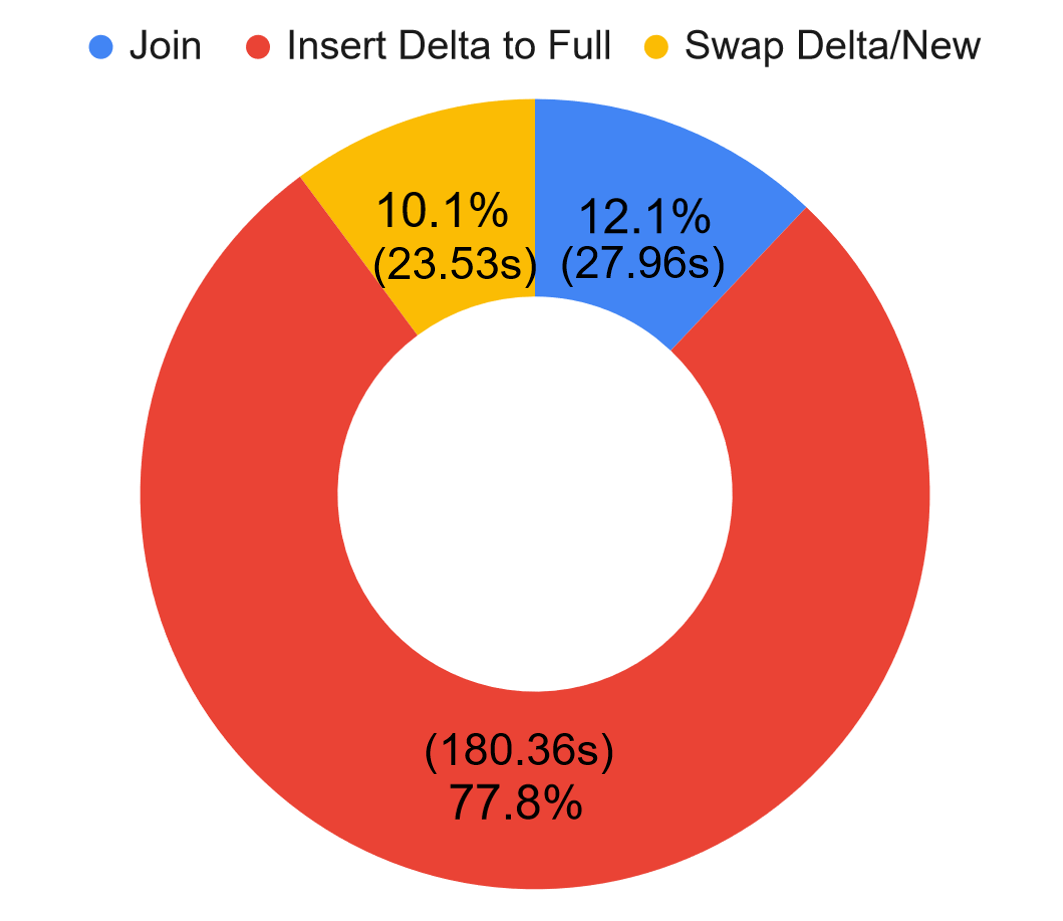
\includegraphics[width=0.7\linewidth]{figures/souffle_detail_ratio.png}
%     \caption{ Runtime Analysis of Souffl\'e: Executing Reachability at 32 threads on the \textsf{com-dblp} dataset with 1.9B edges. }
%     \vspace{-0.3cm}
%     \label{fig:souffle_detail_ratio}
% \end{figure}

% \paragraph*{Datalog on the GPU: Challenges and Opportunities.}

% GPUs and similar hardware accelerators offer an attractive implementation candidate for Datalog backends due to their excellent performance in data-parallel, memory-intensive applications. Their programming model supports highly parallelized loops (with 10,000+ FP32 cores on modern GPUs), making them an apparent match for nested loop joins. Crucially, GPUs provide extremely high throughput: the recent AMD MI300 can transfer 8192 bits in a single clock cycle. Our goal is to use this throughput to sidestep the memory bandwidth limitations faced by CPU-based Datalog engines. % bottlenecks encountered in batch-style in-memory Datalog engines, like Souffl\'e.

% There are several challenges in implementing state-of-the-art Datalog engines on the GPU. First, we need a GPU-based representation of relations (sets of tuples), which are typically implemented via linked data structures on the CPU. Second, the massive number of parallel threads dictates that lock freedom and communication avoidance be particularly relevant concerns. \tool{} uses lock-free data structures by restructuring performance-critical computations (such as sort, join, and merge) into a two-phase process. Since GPUs lack dynamic allocation, our initial pass involves allocating a sizable buffer in the GPU global memory to accommodate the results based on dynamic relation sizes. Next, individual kernel threads perform calculations for their respective segments of the buffer, determined by their unique thread IDs, and proceed to write their corresponding results into the allocated space.

% Along with the chief algorithmic concerns, effectively using a modern GPU involves other challenges such as efficient deduplication of parallel results, minimizing CPU-GPU communication, and optimizing memory coalescing for peak performance. Overcome these obstacles and ensuring performance portability across diverse GPU architectures are essential steps towards creating a high-performance GPU Datalog.

% \paragraph*{GPU Datalog: Prior Work.} There exist several relevant threads of related work in GPU Datalog. However, state-of-the-art work in GPU Datalog often compromise on the expressiveness of full Datalog to achieve their results. For example, Red Fox omits semi-na\"ive evaluation and recursive queries\cite{wu2014redfox}, essential for modern Datalogs.  GPUDatalog employs more similar to the GPU RDBMS GDB~\cite{he2009gdb}, successfully executing such as \emph{REACH} and \emph{SG} by constructing Cache Sensitive Search (CSS) Trees~\cite{rao1999csstree} before each join iteration. Unfortunately,  data organization and storage limits inhibit GPUDatalog's ability to efficiently deduplicate data, and GPUDatalog also eschews semi-na\"ive evaluation.

% More recently was the work of GPUJoin by Shovon et al~\cite{shovon2023towards}. GPUJoin's initial implementation~\cite{shovon2022accelerating} utilized NVIDIA's RAPIDS project cuDF~\cite{cudf}, but struggled with memory-intensive applications due to inefficient memory and buffer management. Its subsequent version improved performance by using an open-addressing hash table for tuple storage, achieving results closer to that of Souffl\'e's interpreted mode~\cite{shovon2023towards}. However, GPUJoin doesn't significantly outperform CPU-based systems---even on modern data center GPUs. Additionally, GPUJoin's data structures are application-specific, significantly impeding expressivity by prohibiting relations with arity greater than two.

% The outcomes from these GPU-based Datalog prototypes have been insufficiently compelling to convince the broader community to transition from CPU to GPU. As a result, adoption of GPU Datalog remain undervalued and underexplored within the community.
 

% Current Datalog prototypes, employing hash tables or non-organized data storage with CCS Trees, fall short in efficiently managing all computation-intensive steps in iterative fixpoint computations. This necessitates compromises, such as forgoing steps like deduplication and multiple arity joins, which disrupts the semi-na\"ive evaluation approach and leads to algorithmic inefficiencies and crucial function absent.


% \begin{figure}[t]
%     \centering
%     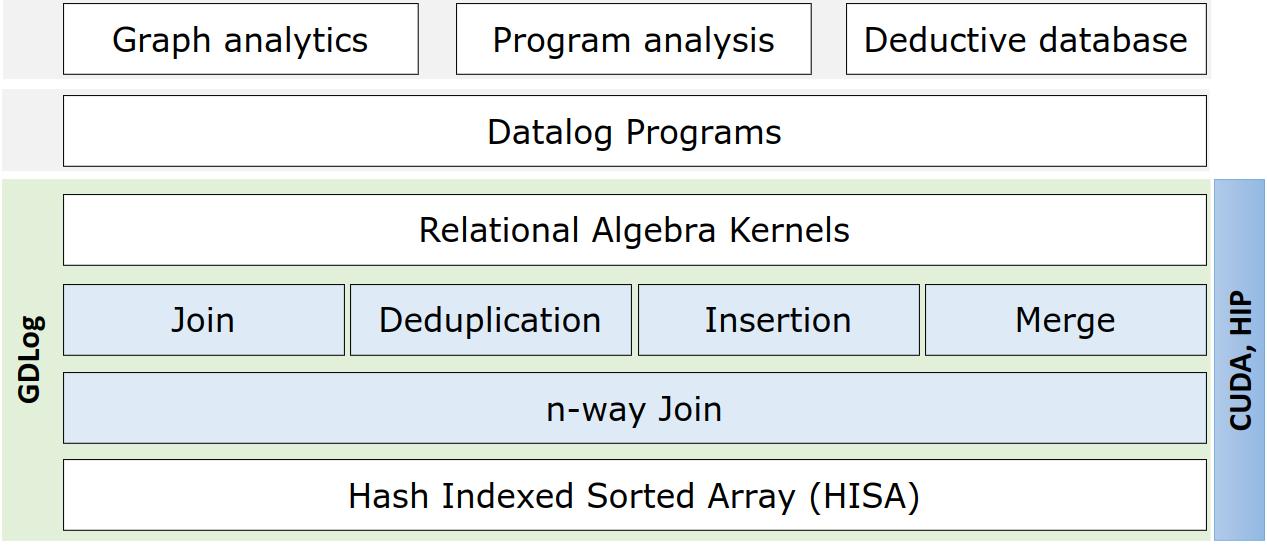
\includegraphics[width=\linewidth]{figures/overview_diagram.png}
%     \caption{ High level block diagram of \tool{}.}
%     \label{fig:overview}
%     \vspace{-0.3cm}
% \end{figure}

% \paragraph*{Our approach}
% Despite the limitations of existing GPU Datalog prototypes, the significant benefits of massive parallelism and the rapid advancement of GPU hardware continue to motivate us in further developing performance portable GPU-based Datalog engines targeting modern heterogeneous computing systems.
% Thus, we have developed \tool{}, a systematic and comprehensive GPU Datalog solution compatible with various data center GPUs.
% % =, as illustrated in Figure \ref{fig:overview}.
% \tool{} is capable of executing Datalog-based applications by translating modern Datalog engine join plans, such as those used by Souffl\'e, into relational algebra operations. It introduces the Hash Indexed Sorted Array (HISA), a data structure optimized for GPUs that supports all the parallel computation phases crucial for semi-na\"ive evaluation. This approach sets \tool{} apart from most existing prototypes, which typically compromise on semi-na\"ive evaluation or essential Datalog language features like multi-ways join and support for relations of multiple arities. 
% In the subsequent sections, we will present the following key features of our implementation:
% \begin{itemize}[leftmargin=*]
% \item Section~\ref{sec:impl-data} introduces our memory-optimized, hash-based indexed data structure (HISA) designed for GPU efficiency.
% \item Section~\ref{sec:gdlog} discusses how \tool{} leverages HISA to implement a scalable and efficient semi-naive evaluation.
% \begin{itemize}
% \item Section~\ref{sec:impl-k-way} describes an efficient implementation of $n$-way iterative joins on new data structure, which has not yet been achieved in existing GPU Datalog research.
% \item Section~\ref{sec:impl-buffer} outlines a trade-off in buffer management in the 2-phase GPU parallel computation.
% \end{itemize}
% \item In Section~\ref{sec:protablility}, we explore \tool{}’s adaptability across various GPU models.
% \end{itemize}

\section{The Hash-Indexed Sorted Array (HISA)}
\label{sec:impl-data}
% \label{sec:impl}

\begin{figure}[t]
    \centering
    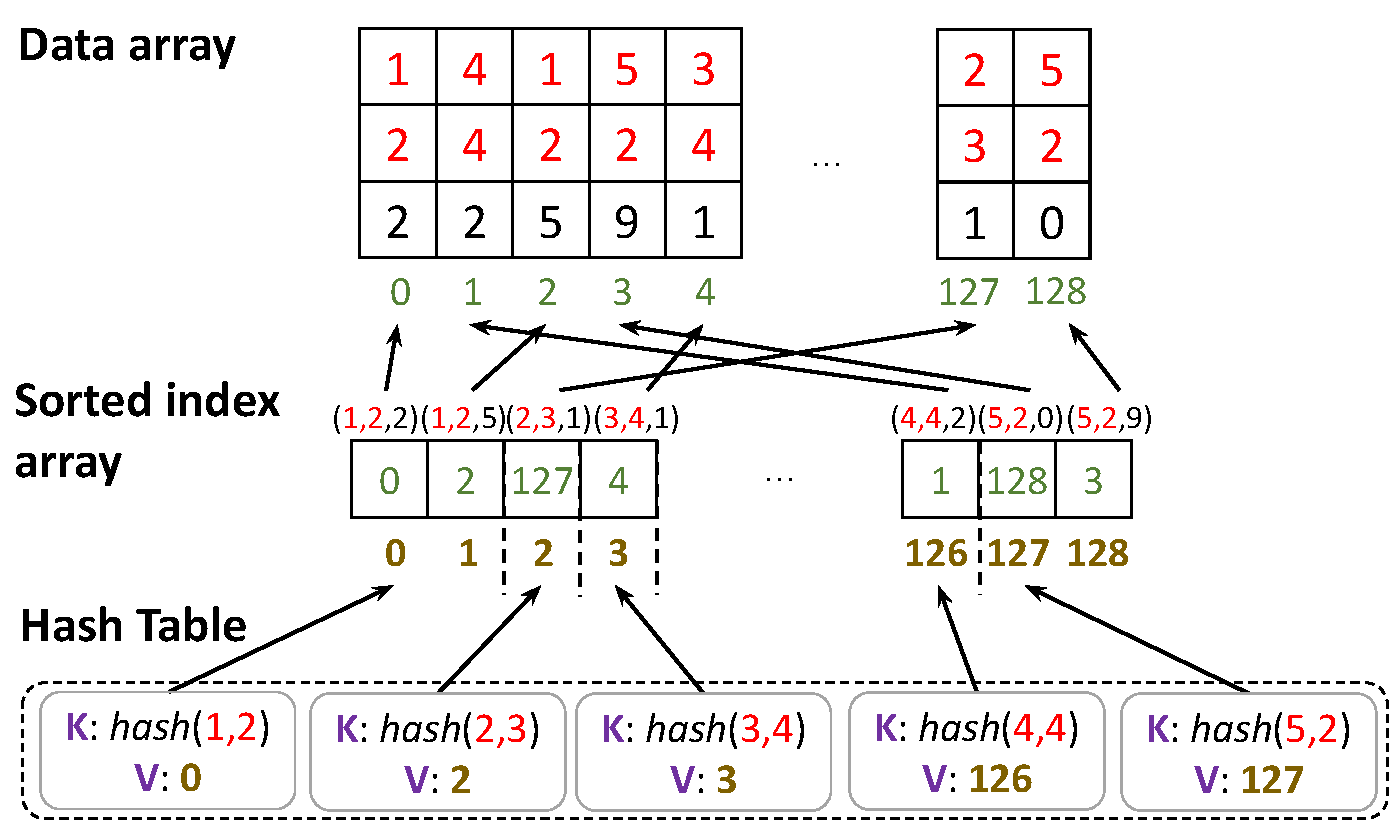
\includegraphics[width=\linewidth]{figures/hisa.pdf}
    \caption{\fontsize{9}{11}\selectfont Example of a 3-arity relation with 2 join-columns (shown in color red) stored in HISA.}
    \label{fig:hisa}
    % \vspace{-0.5cm}
\end{figure}

To meet all four requirements ([R1], [R2], [R3], and [R4]), we developed a novel data structure we call the Hash-Indexed Sorted Array (HISA).
% \subsection{Key components of HISA}
%HISA is a three-layered data structure, comprising a data array, that stores the original tuple data, a sorted index array that stores the indices of the tuples in increasing order, and an open-addressing hash table, built on top of the sorted index array.
%Unlike other data structures where the hash map is built on top of the actual data (tuples), we build our hash map on the sorted index array, while only storing the reference for tuples with unique join column keys. This novel design of the data structure enables fast iteration and fast-range queries while also facilitating deduplication.
%HISA's novel design lies in the way the hash map is built on top of the sorted index array, while only storing the first of the 
%The data array enables fast iterations, the sorted index array is crucial for deduplication, and the hash map enables fast-range queries and facilitates joins on multiple columns. 
HISA, \revised{inspired by~\textit{HashGraph}~\cite{10.1145/3460872}}, is a custom-designed data structure consisting of three interconnected layers. At its foundation lies the data array, which stores the original tuple data. Built upon this data array is a sorted index array, which stores the indices of the tuples in ascending order.
%The tuple indices in the sorted index array are arranged in ascending order based on a lexicographical ordering of the tuples, where the columns are reordered such that the join columns appear first, followed by the remaining columns. 
The third layer is an open-addressing hash table, constructed on top of the sorted index array. HISA is different from other data structures as instead of building the hash table directly on the actual data (tuples), we construct it on the sorted index array. This approach allows us to store references only for tuples with unique join column keys, resulting in a more efficient use of memory.


% Secondly, it supports range-queries, as the hash table built on the sorted index array allows for quick lookups of specific subsets of data. Lastly, by storing the tuples in a sorted order, HISA inherently facilitates deduplication, eliminating redundant data and optimizing storage efficiency.

Figure~\ref{fig:hisa} sketches an example of a HISA data structure at runtime (in VRAM). We will now walk through each of the tiers, and discuss how they collectively enable [R1]--[R4]. 

%Figure~\ref{fig:hisa} shows the key components of HISA. We now present details of each of these components.
%Deduction-heavy workloads on GPUs demand efficient data structures that enable indexing, sorting, and range queries. To meet these requirement, we introduce the Hash-Indexed Sorted Array (HISA), a hybrid SIMD data structure designed for optimal execution of deduction-heavy workloads on the GPU.
%It is inspired by the compact and serializable nature of \textit{HashGraph}~\cite{10.1145/3460872} while tailoring it for Datalog evaluation. At a high level, HISA combines a data array and a sorted index array to support parallel iteration and deduplication, alongside an open-addressing hash table to enable efficient k-arity joins across multiple columns while also facilitating deduplication.

%HISA achieves its performance optimization through a meticulously crafted integration of algorithmic components and data structures.



% a novel k-arity data structure designed for efficient k-arity joins with multiple join columns on the GPU. This data structure combines the benefits of hash tables and sorted arrays which are well-suited for exploiting data parallelism utilizing the GPU architecture. The design of the data structure has three primary steps: 

\subsection{Data Array} 
The \emph{data array} represents the original GPU buffer that stores all the tuples of a relation transferred from the CPU to the GPU.
%The \emph{data array} corresponds to the original GPU buffer that holds all the tuples of a relation passed to the GPU from the CPU.
The $k$-ary relation data can be seen as a 2D array of size $n \times k$, where $n$ is the total number of tuples/rows and $k$ is the number of columns of the relation. An example of this 2D array can be seen at the top of Figure~\ref{fig:hisa}. Here $n = 129$ and $k = 3$, but, for the sake of clarity in exposition, the 2D array is shown in its transposed view. We store this 2D data in row-major order in the GPU buffer. Therefore, the tuples of Figure~\ref{fig:hisa} are stored in a buffer that looks like -- $\{1, 2, 2, 4, 4, 2, 1, 2, 5 \dots, 2, 3, 1, 5, 2, 0\}$.

This densely-packed contiguous arrangement, in contrast to sparse data structures, simplifies access for the GPU. GPU threads can then efficiently perform strided access to underlying the data array.

This simple layout makes it easy to implement parallel data retrieval, addressing the requirement for fast iteration [R2]. 
Coalesced memory access, enabled by our layout, allows multiple GPU threads to fetch data from the same memory block simultaneously, improving cache performance and optimizing memory operations. We provide implementation details of this parallel data access in Section~\ref{sec:gdlog-eval}, in the context of iterating the outer relation for a join operation.

\paragraph*{Merge operation}
\revised{Merging two HISAs typically occurs when combining the full and delta versions of a relation. In semi-na\"ve evaluation, to avoid redundant computation, the delta relation contains only fresh and unique tuples generated in the previous iteration, deduplicated against the full relation. Consequently, when merging delta and full, no additional deduplication is needed—the delta’s data array can be directly concatenated to the full’s data array.}

\begin{algorithm}[t]
\caption{Construction of Sorted Index Array $H_i$ for Relation $H$}
\label{alg:index-construct}
\begin{algorithmic}[1]
% \State Create a new HISA object $H_{i}$
\For{ all tuple $T$ in $H.\text{data\_array}$ \textbf{parallel} }
    \State $\textit{jc} \gets $ [join columns of $T$]
    \State $\textit{njc} \gets $ [non-join columns of $T$]
    \State Insert ($\textit{jc}$ ++ $\textit{njc}$) into $H_{i}.\text{data\_array}$
\EndFor
\State $H_{i}.\text{sorted\_index\_array} \gets $ [0 ... $H.\text{tuple\_size}$]
\For{$i$ in [0 ... $H.\text{arity}$]}
    \State $col_{tmp} \gets$ the $i_{th}$ of column of tuples in $H_i$
    \State stable sort $H_{i}.\text{sorted\_index\_array}$ use $col_{tmp}$ as key
\EndFor
\end{algorithmic}
\end{algorithm}
%\vspace{-0.3cm}

\subsection{Sorted Index Array}
%The middle of Figure~\ref{fig:hisa} showcases a sorted index array, an essential component of the HISA designed for efficient indexing and deduplication. In HISA, tuples are organized in lexicographic order, prioritizing the significance of each column from left to right, for example, $(1,2,2) < (1,2,5) < (5,2,9)$. The sorted index array separates the sorting order of tuples from the data array. It stores the positions of tuples within the data array, and these positions are radically sorted based on the lexicographical order of the tuples they are associated with. For instance, although the tuples $(5,2,0)$ and $(5,2,9)$ may not be positioned adjacently in the data array, their corresponding positions are closely aligned in the sorted index array.

%The detail construction of this array is described as following step:
%\paragraph*{Construction}
%The process begins by initializing the sorted index array with a permutation reflecting the tuples in the data array. The sorting of the index data array then commences, targeting each column of the input tuples. This phase begin with sorting based on the least significant column (the rightmost column) of the tuple as indicated by the index array, and moves towards sorting by the most significant column (the leftmost column). With the  GPU sorting algorithms provided in the NVIDIA Thrust library, this phase achieves rapid and efficient sorting.

%By decoupling the data from its index, the method minimizes the need for intermediate space in parallel sorting tasks and also enables leveraging the radix sort for fast lexicographic sorting. The requirement for indexing fast-range queries ([R1]) in database indexing operations can be met by reordering all join columns to the forefront. This arrangement ensures that tuples with identical joined column values are grouped together. Consequently, once the address of the smallest tuple of tuples sharing the same join columns is identified, the entire set of tuples sharing the same joined column values can be fetched easily by a linear scan from the smallest tuple. 

The sorted index array stores the indices of the tuples from the data array in ascending order. The indices are arranged based on a lexicographical ordering of the tuples. This ensures the join-columns appear first, followed by the remaining columns. For example, consider a $3$-arity data array with tuples $\{2,1,5\}$, $\{2,5,9\}$, and $\{2,1,2\}$, where the second column is the join-column. The corresponding sorted index array would be $1, 0, 2$, because the tuples, after reordering the join column to index 0, follow the lexicographic ordering $(1,2,2) < (1,2,5) < (5,2,9)$. In essence, the sorted index array decouples the sorting order of tuples from their physical arrangement in the data array. It maintains the positions of tuples within the data array, and these positions are sorted based on the lexicographical order of their associated tuples.
% As a result, even if tuples with similar join column values, such as $(5, 2, 0)$ and $(5, 2, 9)$, are not stored contiguously in the data array, their corresponding positions are closely positioned in the sorted index array.

\paragraph*{Construction}
We extensively use NVIDIA's Thrust library \cite{thrust} to perform tasks such as copying, gathering, and sorting. The first step in the process of creating the sorted index array is to reorder the columns, which we perform using Thrust's transform function. This can be seen in line numbers $1$ to $5$ in the Algorithm~\ref{alg:index-construct}. After the reordering phase, we populate the sorted index array, by using Thrust's stable sort utility. This phase performs a stable sort based on the least significant column (rightmost) of the tuple and progresses towards sorting by the most significant column (leftmost). This sorting process is similar to radix sort; however, in this case, tuples are sorted one column at a time (rather than one bit at a time). This can be seen in line numbers $7$ through $10$.

\paragraph*{Fast range-queries}
Rearranging the column order to position the join columns at the beginning and then sorting the tuples offers two significant benefits. First, it enables efficient range queries, and second, it facilitates the fast merging of two relations. While fast-range queries are crucial for performing {join} operations, merging relations is an essential part of semi-na\"ive evaluation. As discussed in Section~\ref{sec:datalog}, the new relation is merged into the full relation at each iteration of the fixed point.

The sorted-index array works in tandem with the hash-map (described in the next subsection) to execute range queries. The hash map directly positions a GPU thread (in O(1) time) at the appropriate location within the sorted index array. Since the sorting process groups together tuples with identical join-column values, a range query can easily retrieve the entire set of tuples sharing the same join-column values by a linear scan.
%
%Rearranging the column order to position the join columns at the beginning and then sorting the tuples has two benefits. First, it enables fast-range queries, and, second, it facilitates efficient merging of two relations. While fast-range query is essential in performing a \emph{join} operation, merging relations is an integral part of the semi-naive evaluation. Recall from Section 1, that new new relation gets merged into the full relation at every iteration of the fixed point.  While the sorted-index array is used in conjunction with the hash-map (next subsection) to perform range queries, where the hash map directly puts a cuda thread (in O(1) time) at the right location in the sorted index array.  Since the sort groups together tuples with identical join columns, a range query where the entire set of tuples with the same join-column values can be easily fetched through a linear scan.
%
%This arrangement groups together tuples with identical join column values, enabling efficient range queries on inner relations. This arrangement groups together tuples with identical join column values, enabling efficient range queries on inner relations. Once the smallest tuple sharing the same join-column is identified, the entire set of tuples with the same join-column values can be easily fetched through a linear scan.
%

% \sout{Merging two HISAs is straightforward: because they are sorted in the same order, an off-the-shelf GPU-based merge algorithm suffices for efficient merging~\cite{green2012merge}. Initially, incoming relation's data array will be directly appended. The sorted index array of the incoming relation is then merged with the existing sorted index array of the original relation. By leveraging the GPU's data parallelism, merging can be performed efficiently, even for large datasets.}

%When two arrays are sorted in the same order, their merging can be efficiently executed in parallel using a GPU-path merge algorithm. This approach enables a parallel bulk insertion process: initially, tuples are appended directly to the data array. Then, the permutations of all incoming tuples are sorted in lexicographic order in parallel. Finally, these sorted permutations are merged with the existing sorted index array.  This method takes full advantage of the parallel processing power of GPUs to optimize the insertion of bulk data into HISA, which will happen in every iteration of Datalog evaluation when merging new tuples into full version of a relation.


\paragraph*{Deduplication}
\label{sec:impl-data-insert}
HISA  supports deduplication [R4] by first sorting all columns in lexical order, facilitating the rapid identification and removal of duplicates. The deduplication process is then executed by comparing each tuple with its adjacent tuple during a parallel scan. This approach ensures both efficient grouping for joins and effective deduplication, leveraging the parallel processing capabilities of the GPU.

\paragraph*{Merge operation}
\revised{Parallel merging of two sorted arrays is a common pattern in GPGPU programming. We utilize the path merge algorithm~\cite{green2012merge} provided by NVIDIA’s Thrust library to merge the sorted index arrays of two HISAs.}


\subsection{Open-Addressing Hash Table}
The sorted index array stores tuples in increasing order, clustering tuples which share the same join-columns.
To further optimize range queries, enabling retrieval of all tuples sharing the same join columns and meeting requirement [R2], HISA incorporates an open-addressing-based hash table. Using a hash table avoids control flow divergence and improves memory access efficiency compared to other range query techniques, such as tree-based searches.

The hash table is constructed to store distinct hash values (as keys) derived from the tuples of the data array, while only considering the join-columns to compute the hash. These keys are then associated with the smallest index of a tuple in the sorted index array (as values) that contains the corresponding join-column values.
An example of this hash table can be seen at the bottom of Figure~\ref{fig:hisa}. In this example, the hash table entry on the far right captures the hash value of join-columns $(5,2)$ and associates it with the starting position of all tuples having the join-column $(5,2)$, indicated by the $127^{th}$ position in the sorted index array.
Instead of directly storing the join column values---which may exceed $64$ bits in size---we opt to store their hash value as the key; this strategy effectively meets requirement [R3].

\begin{algorithm}[t]
\caption{Hash table construction algorithm}
\label{alg:hashtable-construct}
\begin{algorithmic}[1]
\For{each tuple $T$ in input relation, perform in parallel}
\State $H$ $\gets$ $hash(T)$
\State $I$ $\gets$ $H \pmod{\text{hash\_table\_size}}$
\State $T_{pos} \gets$ $\text{get\_position(H, sorted\_index\_array)}$
\While{$T$ is not inserted}
\State $K$, $V$ $\gets$ $\text{hash\_table[I]}$
\State $K' \gets$ AtomicCAS($K$, $H$)
\If{$K'$ $=$ $H$ or $(K,V)$ is uninitialized}
\While{{$T_{pos} < V$}}
\State $V \gets$  AtomicCAS($V$, $T_{pos}$)
\If {$V = T_{pos}$}    
\State \textbf{break} \Comment{Inserted $T$ in $hash\_table$}
\EndIf
\EndWhile

% \While{true}
% \If{$T_{pos} < V$}
% \State $V \gets$  AtomicCAS($V$, $T_{pos}$)
% \If {$V = T_{pos}$}    
% \State \textbf{break} \Comment{Inserted $T$ in $hash\_table$}
% \EndIf
% \Else 
% \State \textbf{break}
% \EndIf
% \EndWhile
\Else
\State Perform linear probing on $I$
% \State $I$ $\gets$ $I+1$$\pmod{\text{hash\_table\_size}}$ 
% \State
% \Comment{ Collision: linear probing}
\EndIf
\EndWhile
\EndFor
\end{algorithmic}
\end{algorithm}

\paragraph*{Construction} 
The pseudo-code for the construction of the hash table can be seen in Algorithm~\ref{alg:hashtable-construct}. We construct an open-addressing hash table, employing linear probing to handle collisions. The keys of the hash table are generated from the data array, while the values are derived from the sorted index array. 
%GPU threads access all elements of the data array via iterating through the sorted index array and referencing to the date array (line 1), computing the hash for each set of join-column values (lines 2 and 3). These hash values serve as the keys for the hash table, and the corresponding values are the positions of those keys in the sorted index array (line 4). 
GPU threads go through the sorted index array, which allows them to access all elements of the data array. They calculate hash values for every tuple, using only the join-column values and use these hash values as keys in the hash table. The hash table's values store the positions of the corresponding keys in the sorted index array, enabling quick lookup and access to the relevant data elements.
To handle collisions that occur when two keys map to the same slot in the hash table, we employ linear probing. However, since insertion is performed in parallel by thousands of threads, it is possible that during collision resolution, two threads with hash collisions attempt to write to the same hash slot.
To address this challenge, we utilize the \texttt{atomicCAS} (Compare-and-Swap) operator at line 7 of the algorithm, which ensures that only one thread can successfully update a slot at a time.
%As is with any hash table, a collision occurs when two keys are mapped to the same slot in the table, to overcome this challenge we using linear probing, however, since insertion in our case is happening in parallel by thousands of threads, we must avoid race conditions when a thread overrides data from other threads. To solve this issue we extensively rely on the usage of atomicCAS operator.
%In instances where two hash values map to the same entry, the collision is resolved using a linear probing as can be seen in the while-loop, fom lines $5$ to $22$.
%Actual insertion of key-value pairs are performed using \texttt{atomicCAS} (atomic compare and swap)~\cite{} operator to ensure that threads do not override each other.
%that ensuresin the has tables 
%which searches for the next available hash table slot.

% The way we have designed our hash table, among the tuples with the same join-column values, we only store the position of the smallest one.
In parallel execution, multiple GPU threads update smallest index of a tuple in the sorted index array simultaneously. This also leads to a race condition when two tuples sharing identical join column values are concurrently inserted into the hash table by two separate GPU threads.  We handle this from line 9 to line 14 of the algorithm, also using \texttt{atomicCAS} operator, which updates a value only if the new key-value pair is smaller than one existing in the hash table.

%To manage this race condition in a lock-free manner, a while-true-loop at line $8$ coupled with a check at line $11$ ensures a successful update. 
%If the exchange is successful, implying the new new key has replaced an existing one needs to be identical to the return value of the \texttt{atomicCAS} function, upon which the algorithm will terminate. This loop continues until the existing value is either smaller than the new value or the swap is successful, thus guaranteeing a consistent update.

%This construction process is executed through a parallel CUDA kernel applied to every tuple in the data array. Within this kernel, line 1 involves calculating the hash value of the joined columns. Then, to find the corresponding entry in the hash table, we apply the modulus operation on the hash value with the size of the hash table in line $3$. 

%After the hash collision is resolved, GPU threads compare the sorted index array position with the value currently found in the hash table entry, as shown in line $4$. If the new value is smaller, it will be atomically exchanged with existing value at line $10$, if not algorithm break back into parallel for loop at line 13.
%A potential race condition arises when two tuples sharing identical index column values are concurrently exchanged into the hash table by two separate GPU threads. To manage this race condition in a lock-free manner, a while-true-loop at line $8$ coupled with a check at line $11$ ensures a successful update. 
%If the exchange is successful, the value exchanged needs to be identical to the return value of the \texttt{atomicCAS} function, upon which the algorithm will terminate. This loop continues until the existing value is either smaller than the new value or the swap is successful, thus guaranteeing a consistent update.

% If the exchange is successful, value exchanged in need to be identical to the return value of \texttt{atomicCAS} function, and algorithm will return.

To conduct a range query, the process begins with calculating the hash value of the join columns. Based on this hash value, the method navigates to the smallest tuple possessing the specified join-column values and then proceeds with a linear scan until encountering a tuple where the join-column value no longer matches. We show this in more detail in the context of a join operation in Section V.A.
% This mechanism enhances data fetching efficiency by leveraging the hash table for quick access to grouped tuples, significantly improving performance on GPU architectures by reducing the need for incoherent memory access and branching. 

\paragraph*{Merge operation}
\revised{Currently, hash table merging of HISA is done by inserting all elements from the Delta hash table into the Full table. For each existing key, the value is updated if the Delta value is smaller than the current value in the Full hash table. While we consider  more efficient algorithms (e.g., Cuckoo Hashing\cite{li2021dycuckoo}) as an important future direction, GPU hash tables can process up to 0.5 billion keys per second, making this approach faster than merging sorted arrays, which requires significant time for buffer allocation and deallocation during path-merging. }

% \begin{algorithm}
% \caption{Hash table construction algorithm}
% \label{alg:hashtable-construct}
% \begin{algorithmic}[1]
% % \State Initialized all hash entry key using U64\_MAX
% \For{each tuple $T$ in input relation perform parallel}
% \State Calculate hash value $H$ for tuple $T$
% \State Calculate index $I$ as $H \pmod{\text{index map size}}$
% \State $T_{pos} \gets$ position of H in data arrary
% \While{true}
% \State Check key $K$ and value $V$ at index $I$ in hash table
% \If{$K$ equals $H$ or $(K,V)$ is not initalized}
% \State Atomic updating using following loop:
% \While{true}
% \If{$T_{pos} < V$}
%     \State $V \gets$  AtomicCAS($T_{pos}$, $V$)
%     \State \textbf{if} $V = T_{pos}$ \textbf{return}
% \Else ~ \Return
% \EndIf
% \EndWhile
% \State \textbf{break}
% \Else
% \State Increment $I$

% \EndIf
% \EndWhile
% \EndFor
% \end{algorithmic}
% \end{algorithm}

% \While{true}
% \If{$V$ $<$ $I$ and tuple at $V$ != $T$}
% \State Collision detected, increment $I$
% \State Continue outer loop
% \EndIf
% \If{$V$ greater than tuple index}
% \State Swap $V$ with tuple index of $T$
% \EndIf
% \State \textbf{break} inner loop
% \EndWhile
% \State Insert $(H, H_{pos})$ into hash table at $I$

% . Sorting simplifies the data structure merge operation, as it boils down to merging sorted values in the indexing map. This merging process is also highly GPU-friendly, achieved by coarsely partitioning the indexed map into several sorted chunks in GPU memory and merging them with fast parallel primitives.
% Overall, this sorted merge design harnesses the strengths of the GPU for massively parallel sorting, scanning, and merging and significantly enhances the efficiency of the deduplication operations in the fixed-point iterations.

% \paragraph*{Efficient range querying and serialization}
% Inductive queries in Datalog, which entail iterative fast range queries on indexed columns, benefit from hash-based indexing. This method, offering \textit{O(1)} range fetching time, is significantly advantageous over sort-merge joins.
% Storing only the join column data in the hash table enables us to achieve efficient insertion and retrieval operations based on key values. 
% To address the serialization requirements during operations such as recursive joins on the GPU, and merging delta data into the full dataset, HISA’s compact sorted data array become useful. Serialization can be efficiently executed through parallel iteration over this structured array.
% Moreover, the hash table only contains the columns required for joins, not the full tuples. This optimization significantly reduces memory usage while still ensuring fast join performance. The hash table construction is shown in Algorithm \ref{alg:hashtable-construct}. The bulk of the data is stored in a scalar array tailored for GPU architecture. Simultaneously, for inner relations that require fast range queries, we employ a hashmap designed to store only the indexed columns and the address of the smallest tuple pertaining to that indexed column. This approach optimizes space utilization while maintaining the efficiency of range queries, a key consideration in the context of Datalog and similar declarative languages. While \textit{HashGraph}~\cite{10.1145/3460872} demonstrates the effectiveness of combining a hashmap with a compact array-style data structure on GPU, it does not directly align with the specific demands of Datalog. Notably, it lacks support for handling multi-values and deduplication, which are essential aspects of Datalog queries. HISA addresses these limitations by introducing a sorted hash-indexed table mapped with the compact data array. This innovation allows us to utilize mainstream GPU merge and sort algorithms. By combining the sorted index map with the compact data array in this manner, we obtain a high-performance data structure tailored to the needs of recursive joins on the GPU. HISA's design aims to provide the best of both worlds - efficient indexing and high-performance data manipulation - to support Datalog workloads on GPU architectures.



\section{\tool{}: GPU-powered datalog engine}
%Using HISA for Datalog on the GPU}
\label{sec:gdlog}

In this section, we introduce \tool{}, our GPU-accelerated implementation of Datalog that leverages the HISA to optimize performance and efficiently utilize the GPU. We focus our discussion on three distinguishing aspects: (a) implementation of the semi-na\"ive evaluation in the fixed-point loop, (b) a novel optimization to significantly accelerate $n$-way joins: temporary materialization, and (c) eager buffer management, which leverages amortization to improve memory allocation.

\begin{figure}[]
    \centering
    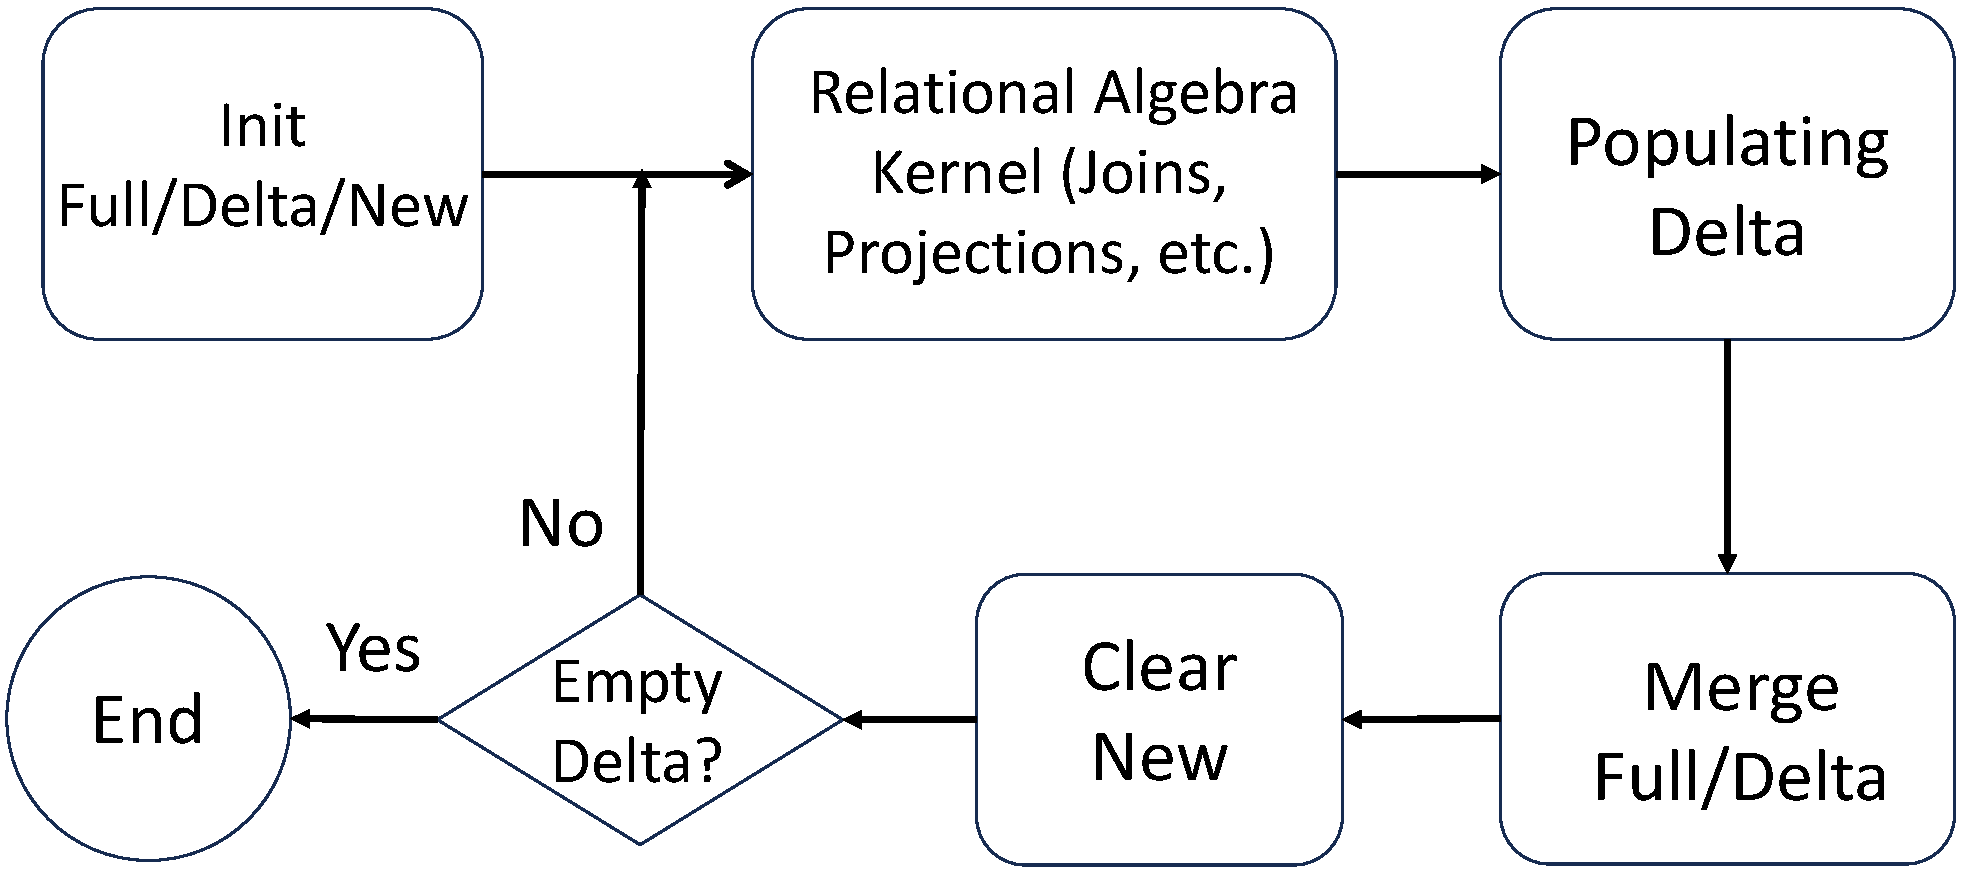
\includegraphics[width=0.78\linewidth]{figures/eval_flow.pdf}
    \caption{\fontsize{9}{11}\selectfont Workflow of semi-na\"ive evaluation.}
    \label{fig:eval-flow}
\end{figure}

\subsection{Evaluation of Datalog Programs}
\label{sec:gdlog-eval}
%GDLog implements the semi-naive evaluation workflow as described in Section~\ref{}. Figure~\ref{fig:eval-flow} delineates \tool's evaluation workflow, which comprises five distinct phases: "Updating Index", "Join", "Populate Delta", "Merge Full/Delta", and "Clear New".

Datalog's evaluation is often given in terms of relational algebra, which includes relational operators such as join and projection. Evaluation executes these kernels in a loop. In each iteration of the loop, compute kernels (compiled from the program rules) generate new tuples (facts); these newly-discovered facts may then trigger further deduction in subsequent iterations. The process continues until a fixed point is reached, where no new facts can be derived. Figure~\ref{fig:eval-flow} illustrates the detailed steps involved in this evaluation process, namely ``Join,'' ``Populate Delta,'' ``Merge Full/Delta,'' and ``Clear New.''


%\paragraph*{Updating Index}
%Within a Datalog program, it's common for each relation to be associated with multiple indexes due to the variety of ways it might be queried or joined. Taking the Same Generation query as an example, as described in Section~\ref{sec:datalog}, the \textit{SG} relation undergoes joins on both its first and second columns, thus requiring the generation of two distinct indexes for \textit{SG}. In essence, we create two HISA data structures for the edge relation, one indexed on the first column and the other indexed on the second column. 
%\tool{} ensures that all incremental changes to a relation are accurately reflected across all its indexes. 



\paragraph*{Implementing Joins}
\label{sec:join-impl}
% The second step in the fixpoint computation involves the execution of join operations in \tool{}.
% Leveraging our hybrid data structure, these join processes are designed to harness the benefits of both hash and sorted joins, making them well-suited for recursive query scenarios on GPUs.
The bulk of the evaluation overhead of modern Datalog evaluation lies in iterated joins. For example, consider the following query:
%We illustrate the implementation of the \emph{join} operation, through following query: 
\[
\begin{array}{lcl}
    \textit{Foobar}(c,d)  & \leftarrow &  \textit{Foo}(a, b, c), \textit{Bar}(a, b, d). 
\end{array}
\]
This join operation involves two relations, each with three attributes, sharing the first two columns as join columns in Figure~\ref{fig:join_layout}.
To facilitate parallel iteration over all tuples of the outer relation, we use the data array component of the HISA data structure.
As shown in the figure, we access the data array of the outer relation in \emph{stride} units. The size of each stride corresponds to the total number of threads employed for concurrent execution. 
Each GPU thread concurrently retrieves a tuple within a stride, where the thread ID corresponds to the tuple's offset within that stride.
In the example shown all tuples of the outer relation are accessed in two strides, the first stride ranges from tuples $\textit{Foo}(2,3,5)$ to $\textit{Foo}(5,2,4)$ and the second stride ranges from $\textit{Foo}(2,3,2)$ to $\textit{Foo}(5,2,6)$. We encapsulate this strided access in the form of a parallel for in line number $1$ of the Algorithm~\ref{alg:join}.
Users can configure the stride size based on their GPU, with a recommended size being $32$ times the number of stream processors.
By accessing the data in the outer relation using this stride-based approach, data locality is improved, leading to optimal utilization of the cache and enhancing overall performance.

\begin{figure}[t]
    \centering
    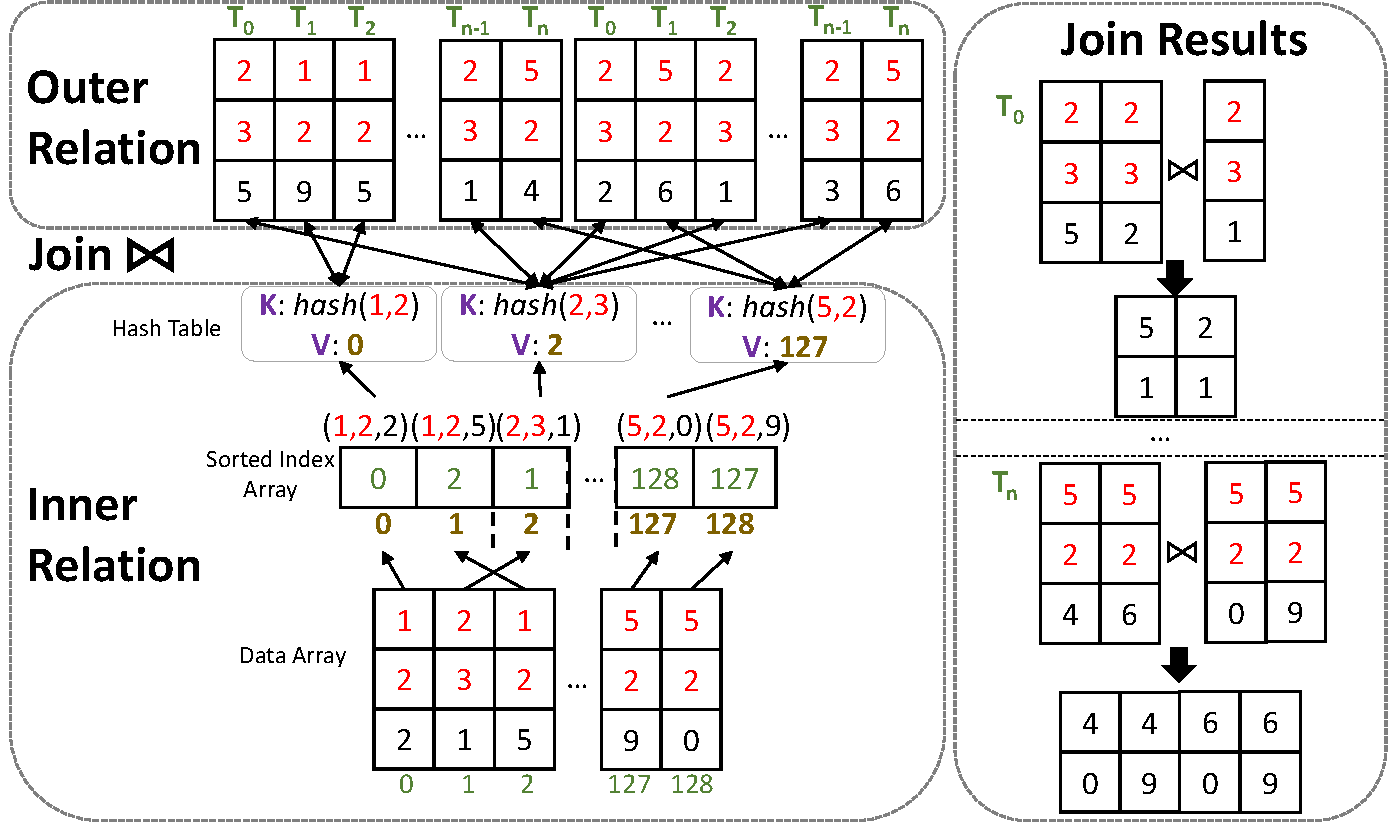
\includegraphics[width=1\linewidth]{figures/join_layout.pdf}
    \caption{Example of a join between two 3-arity relations \textit{Bar} (inner) and \textit{Foo} (outer).}
    \label{fig:join_layout}
    % \vspace{-0.2cm}
\end{figure}
The lower section of the figure demonstrates how each thread queries the inner relation.
The range queries are facilitated by using the hash table and the sorted index array components of HISA. 
The hash table is used to find the starting position of the relevant queries in the sorted index array (lines $2$ to $5$), which is then linearly scanned to retrieve all matching tuples from the data array (lines $6$ to $10$).
For instance, thread $T_0$ operates on the outer relation tuple $Foo(2,3,5)$ and $Foo(2,3,2)$.
After hashing column $(2,3)$, \tool{} uses the hash table of the HISA structure to find the smallest tuple at position $2$ in the \textit{Bar} relation's sorted index array, yielding $\textit{Bar}(2,3,1)$. A scan starting from this position reveals that the only matching tuple in the \textit{Bar} relation is $\textit{Bar}(2,3,1)$. On the right side of the figure, the join results show that tuples $\textit{Foobar(5,1)}$ and $\textit{Foobar(2,1)}$ are generated as a result of the join between matched tuples from the outer and inner relations.

\revised{
Although both employ hash join-like algorithms, \tool{} differs from the join algorithm used in another Datalog engine prototype, GPUJoin~\cite{shovon2023towards}. In GPUJoin, the hash table directly contains all tuples, and during the join, tuples are accessed through linear probing of the hash table. This design can lead to larger hash tables and increased memory overhead, especially when a low load factor is used for faster construction. In contrast, our tool’s join algorithm accesses the hash table only to find the starting position of tuples sharing the same indexed column. This approach keeps the hash table size small and allows for fast construction.
}


%and array ensures coalesced memory access, optimizing memory operations on the GPU.
%This stride-based approach to accessing the data array ensures coalesced memory access, optimizing memory operations on the GPU.
% Once the data is partitioned, each GPU thread can readily access tuples within the stride array according to its unique thread ID number. Thanks to \tool{}'s sorted array storage of relation tuples, the process of serializing and partitioning a relation becomes streamlined\shovon{should we remove "compact"}. This stands in contrast to a pure hash join, where efficiently iterating over the hash table and optimizing the distribution of join operations poses a significant challenge.

% During the join process, each thread calculates the hash value of the join columns, queries the inner relation's indexing hash table, and locates the smallest tuple sharing the same join columns. Since all tuples are sorted, a linear scan of the relation's internal array starting from the smallest tuple offset facilitates the join.


% It computes the hash value of the indexed column (in this case, the first column), which results in the value 0x370ca71c\shovon{Fig 4 shows hash(x, y) rather than actual hash value. do we need to follow that in fig 6?}. It then queries the indexing hash table of inner relation $Edge_{2,1}$ with this value and discovers that the smallest tuple with 1 as its first column is located at offset 0 in the internal array of relation $Edge_{2,1}$. Subsequently, a scan of the sorted data array facilitates the join of the tuple $Edge_{2,1}(1,2)$ and $Edge_{2,1}(1,5)$, generating join result tuples $Reach(3,2)$ and $Reach(3,5)$. 
% It is important to note that while we can obtain the join result at this point, due to GPU limitations, on-the-fly buffer allocation is not possible. The standard practice, also adopted by other works such as RateupDB \cite{lee2021rateupdb} and GPUJoin \cite{shovon2023towards}, is to repeat the above join operation twice. The first pass is used to compute the size of the join result, followed by writing the join result into the result buffer during the second round.

% Before storing the join results in the new version of the output relation, an important additional step is the deduplication of join results in each iteration, so that no repetitive computation is done in the next iteration. %This important step is not implemented effectively in existing GPU-based deductive engine prototypes (such as Red Fox). 
% \tool{} accomplishes this by utilizing sorting based on the lexicographic order of tuples \shovon{already described in ~\ref{par:dedup}}, followed by a scan to eliminate sequential duplicates. Both of these operations are parallelized by the GPU and are readily implemented using functions from NVIDIA's Thrust library.


\begin{algorithm}[t]
\caption{Parallel Binary Join on GPU}
\label{alg:join}
\begin{algorithmic}[1]
\For{$T_{outer}$ in $\textit{Relation}_{outer}$ \textbf{parallel}}
    \State $\textit{ht} ~ \gets$ hash($T_{outer}$.join\_columns)
    \State $\textit{index\_pos} \gets \textit{ht} ~ \% ~$ hash table size of $ \textit{Relation}_{inner}$
    \State $\textit{pos} \gets \textit{Relation}_{inner}$.sorted\_index\_array[\textit{index\_pos}]
    \State $T_{inner} \gets$ tuple at \textit{pos} in $\textit{Relation}_{inner}$.data\_array
    \While{$T_{inner}.$join\_columns $\neq T_{outer}$.join\_columns}
        \State generate result tuples based on $T_{outer}$ and $T_{inner}$
        \State \textit{pos}++
        \State $T_{inner} \gets$ tuple at \textit{pos}
    \EndWhile
\EndFor
\end{algorithmic}
\end{algorithm}

\paragraph*{Populating delta}
\label{sect:pop-delta}
The next step in the fixpoint loop involves populating the \textit{delta} relation, which will be used in the join phase of the next iteration. \revised{In this step, \textit{delta} is constructed by removing from \textit{new} the tuples that are already present in \textit{full}.} \tool{} accomplishes this using a relational algebra ``set difference'' applied to the \textit{new} and \textit{full} relations.
It is worth noting that some prior work, such as GPUJoin, fuses this step with the merging step by directly merging the non-deduplicated \textit{delta} relation and then deduplicating the merged \textit{full} relation. This fusion approach is efficient when the size of the \textit{full} relation is small. However, deduplicating the \textit{full} relation requires a full scan of all the tuples in the \textit{full} relation, which becomes highly expensive as the size of the \textit{full} relation grows. Therefore, \tool{} takes a different approach by separating the \textit{delta} relation population into a distinct phase.

\paragraph*{Merging Full with Delta and Clearing New}
The final step before fixpoint checking involves merging all the tuples within the \textit{delta} relation into the \textit{full} relation, followed by the removal of all tuples within the \textit{new} relation. Leveraging the HISA bulk insertion technique outlined in Section~\ref{sec:impl-data-insert}, we incorporate all deduplicated new tuples from \textit{delta} into \textit{full} in parallel on the GPU.
It is worth noting that the management of buffer memory during merging between \textit{full} and \textit{delta} plays a crucial role in ensuring the optimal performance of larger queries. %Subsequently, we will delve into the finer details of this memory management strategy in the following subsection.

% As we have previously discussed in the background and motivation ~\shovon{should we use ref?} section, this particular phase is inherently serial and has the potential to become a bottleneck when dealing with larger query sizes in CPU-based Datalog engines. In \tool{} we can take advantage of GPU operation over our data structure's internal compact array to parallelize this process.
% Efficient parallelization is achieved by employing a strategy that entails the coarse yet swift partitioning of both the sorted array of \textit{full} and \textit{delta} relations into several small, sorted tiles, each of which can fit neatly into a GPU's execution wraps. This transformation of the merging process effectively converts it into a divide-and-conquer problem and, as a result, makes it amenable to seamless acceleration by SIMD hardware.


\subsection{Temporarily-Materialized $n$-way Joins}
\label{sec:impl-k-way}
% The second type of trade-off occurs when more than 2 relations are involved in a join. 
While simple Datalog queries use only binary joins, practical applications include $n$-way joins. An example is the Same Generation (\emph{SG}) query  mentioned in Section~\ref{sec:datalog}. 
The second rule of \textit{SG} represents an inductive case that necessitates joining \emph{SG} with \emph{Edge} twice. When employing semi-na\"ive evaluation, its join plan may be expressed via the following relational algebra operation:
\begin{displaymath}
\begin{array}{lcl}
        \textit{SG}_{\emph{new}} & = & \textit{Edge}_{\emph{full}} \bowtie \textit{SG}_{\emph{delta}} \bowtie \textit{Edge}_{\emph{full}} 
    \end{array}
\end{displaymath}
Various mechanisms exist for evaluating $n$-way joins; while special-purpose joins (such Leapfrog Triejoin~\cite{veldhuizen2014leapfrog}) can achieve worst-case optimal bounds, they do so by imposing representation restrictions. Modern engines tend to favor nested-loop joins~\cite{jordan2016souffle}, in which case $n$-way joins are ordered into sequences (or trees) of binary joins, with an emphasis on optimizing the join order\cite{zhao2024evaluating}. In the case of \emph{SG},  it first loops over  $\texttt{Edge}_{\emph{full}}$ and within the loop body, it further loops on all matched  tuples in $\texttt{Edge}_{\emph{delta}}$. This generates another nested loop over to join with $\texttt{Edge}_{\emph{full}}$.
% there are three distinct methods (unique combinations of 3 join candidates) for dividing the join into sub-joins and allocating them across threads.  For example, one strategy involves partitioning the entire join based on tuples in the outermost relation (\emph{i}.\emph{e}., tuples in $\texttt{SG}_{\emph{delta}}$).

% Multi-core CPUs operate on a Many Instruction Many Data (MIMD) architecture, allowing each thread to execute different instructions concurrently without experiencing idle time caused by conditional branching in the program. However, this workload division approach doesn't align with the hardware nature of GPUs. GPUs utilize a Single Instruction Many Data (SIMD) architecture, where threads within the same GPU warp can only execute the same instruction at any given time.
Due to the architecture of GPU, conditional branching in the program can lead to threads idling during an $n$-way join.
For example, in Figure~\ref{fig:join_imbalance}, thread $T_0$ is assigned to compute the join result for the tuple $\texttt{SG}(2,4)$. During the first join with $\texttt{Edge}_{\emph{full}}$, it generates numerous temporary results. Unfortunately, thread $T_{n-1}$ and thread $T_{n}$ lie within the same GPU warp and do not find any matching tuples. In the subsequent join between the first set of join results and $\textit{Edge}_{\emph{full}}$, $T_0$ must continue the computation, while threads $T_{n-1}$ and $T_n$, have to remain idle until $T_0$ completes the second join and returns.

\begin{figure}[t]
    \centering
    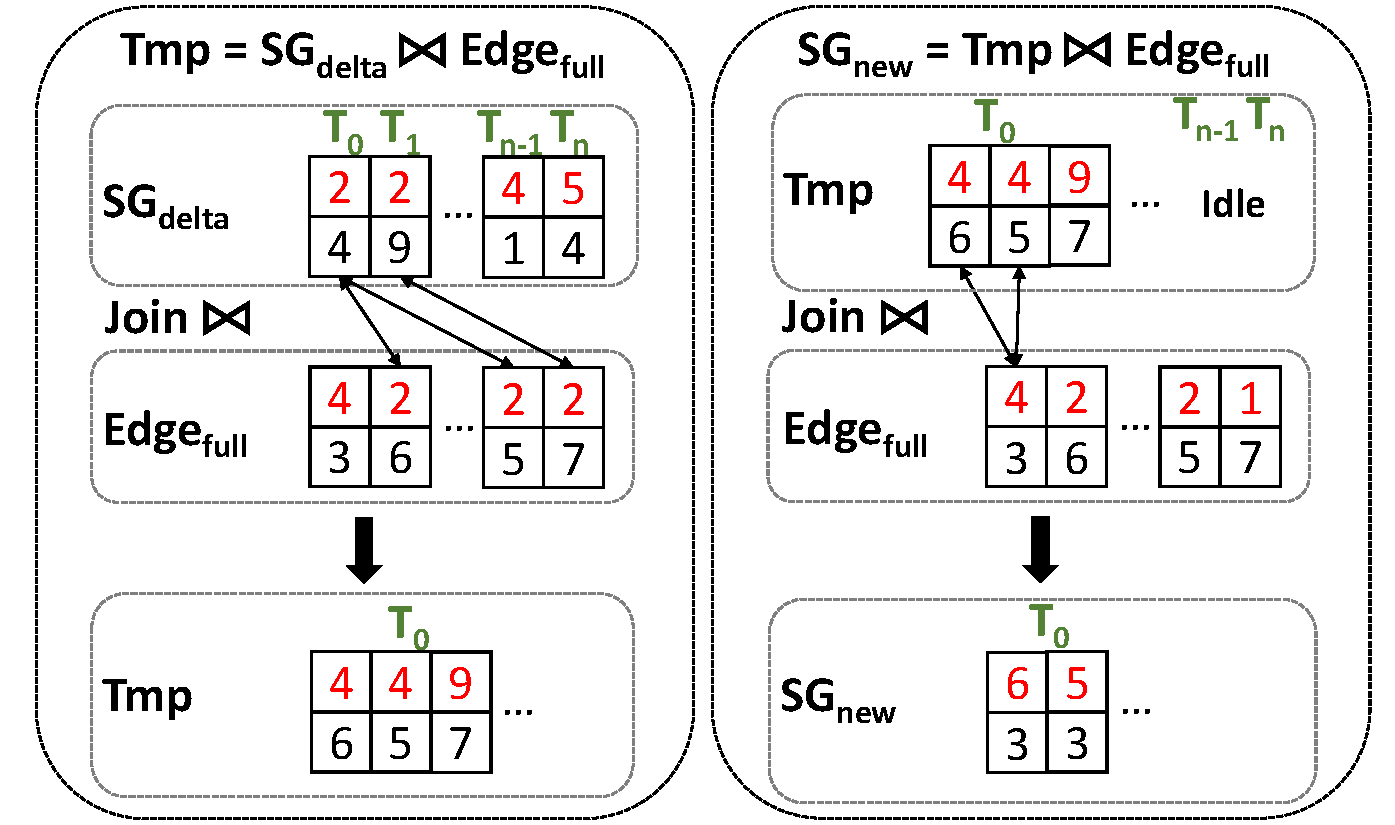
\includegraphics[width=0.9\linewidth]{figures/join_imbalance.pdf}
    \caption{Thread waiting in nested non-materialized join due to workload imbalance. $T_0$ to $T_n$ are in the same warp.}
    \label{fig:join_imbalance}
\end{figure}

Another approach to divide the workload among threads involves materializing each sub-join. We leverage this observation by using a ``temporary materialized'' buffer. In \textit{SG}, the second rule can be seen as two sequential binary joins:
\[
    \begin{array}{lcl}
        \textit{Tmp}(b, x) & \leftarrow & \textit{Edge}(a,x), ~ \textit{SG}(a, b).  \\
        \textit{SG}(x, y) & \leftarrow & \textit{Edge}(b, y), ~ \textit{Tmp}(b, x).
    \end{array}
\]
In relational algebra, an explicit join plan may be written as:
\[
    \begin{array}{lcl}
        \textit{Tmp} & = & \textit{SG}_{\emph{delta}} \bowtie \textit{Edge}_{\emph{full}} \\
        \textit{SG}_{\emph{new}} & = & \textit{Tmp} \bowtie \textit{Edge}_{\emph{full}}
    \end{array}
\]
This split does not make a significant impact on performance for CPU based system. However, in GPU-based systems, having two sequential joins scheduled into two separate executions of GPU kernel functions is notably faster from the first method, where only one GPU kernel function executes. By utilizing the technique of temporal materialization, data parallelism is optimized to its fullest extent. This optimization ensures that all available threads are actively engaged in computation, effectively eliminating any idle time.

The first join's workload is based on tuples in $\textit{SG}_{\emph{delta}}$. By contrast, the workload of the second join is \revised{divided} based on the $\textit{Tmp}$  tuples. In the previous example, temporary join result tuples like $\textit{Tmp}(9, 7)$ are assigned to other idle threads, such as thread $T_{n-1}$, $T_n$, rather than all being processed by the busy thread $T_0$. In this way, all threads in the same GPU wrap will have a similar workload, eliminating idle threads.

%By utilizing the technique of temporal materialization, data parallelism is optimized to its fullest extent. This optimization ensures that all available threads are actively engaged in computation, effectively eliminating any idle time.

% The main drawback to temporarily-materialized joins is the extra space overhead required  to store the temporary relations. However, unlike in shared-nothing approaches (such as BPRA~\cite{kumar2020load})---wherein intermediate results must be persistently materialized in space---our approach purges temporarily tuples once the associated join completes.
% Additionally, unlike normal relations, temporarily-materialized results do not require multiple versions, sorting, or deduplication.


\subsection{Buffer Management and Amortized Allocation}
\label{sec:impl-buffer}

\revised{As we will see in Section~\ref{sec:eval-buffer}, the merge operation of \emph{delta} tuples into the \emph{full} version of the relation becomes a bottleneck, consuming up to 45\% of the total execution time. Buffer management during the merge process is particularly expensive, as it requires reallocating new buffers and copying data equivalent to the combined size of the \emph{full} relation and the \emph{delta} for each iteration. To address this, \tool{} employs a strategy called Eager Buffer Management (EBM).
Unlike the buffer management policies in other GPU Datalog engines, such as GPUJoin, the buffer allocated using EBM in \tool{} is not freed immediately after the merge operation. Before performing the merge, \tool{} checks if the buffer allocated in the previous iteration is sufficient for the current merge operation. If it is, the buffer is reused; if not, rather than allocating a buffer with the exact size of the full and delta tuples, \tool{} allocates a buffer sized to the full tuple size plus \textit{k} times the delta tuple size, where  $k$  is a tunable parameter depending on the total size of VRAM. This strategy reduces the overhead of frequent buffer allocations in every iteration and uses a small amount of extra memory to enable faster iterative computation.}
% EBM pre-allocates a larger-than-necessary buffer during the initial merge phase. This buffer can later be reused across multiple iterations,  amortizing allocation time. 

% Algorithm~\ref{alg:buffer-alloc} formalizes EBM's allocation strategy. The algorithm runs each iteration, and begins by checking whether the existing buffer size is sufficient to accommodate the \textit{delta} tuples generated in the current iteration in addition to the pre-existing tuples (in the \textit{full} relation). If so, the buffer is reused. Otherwise, \tool{} expands the buffer by $\textit{fullSize} + \textit{deltaSize} \times K$; $K$ is initially set to $5$. The algorithm then checks whether the proposed buffer size exceeds the available GPU memory size. If the candidate size is too large, the algorithm gradually reduces $K$ until it can fit within the remaining GPU memory. If $K$ is reduced to $0$, it indicates that there is insufficient GPU memory to complete the join operation, leading to an ``Out of Memory'' (OOM) exception.% exception being thrown. %This proactive approach optimizes memory allocation for efficient semi-na\"ive evaluation.


%In real-world queries, the size of the delta relation tends to gradually decrease in the last few iterations toward the final fixpoint. During these tail iterations, creating buffers becomes a costly operation because the full relation contains a considerable number of tuples.
%\buffer effectively reduces the buffer allocation overhead during these tail iterations, while introducing only a small amount of additional memory overhead.



% Although To reuse buffers, GDlog may needs to maintain these buffers can lead to additional GPU memory consumption (1.35x more according to our benchmark), it represents a deliberate space-for-time trade-off. 


% \algrenewcommand\algorithmicrequire{\textbf{Input:}}
% \algrenewcommand\algorithmicensure{\textbf{Output:}}
% \begin{algorithm}[t]
% \caption{Allocate buffer for merging delta and full. \revised{Replace "Requrie/Ensure" with "Input/output"}}
% \label{alg:buffer-alloc}
% \begin{algorithmic}[1]
% \Require allocatedBufferSize, deltaSize, fullSize
% \Ensure currentMergeBuffer
% \If{allocatedBufferSize $<$ deltaSize + fullSize}
% \State \Return currentMergeBuffer
% \EndIf

% \State $K \gets \alpha$ \Comment{We set $\alpha = 5$}
% \State \textit{freeMemory} $\gets$ \textit{getFreeGPUMemory}()

% \While{\textit{fullSize} + \textit{deltaSize} $\times$ K $<$ \textit{freeMemory}}
% \State $K$ $\gets$ $K-1$
% \If{$K = 0$}
% \State \textbf{throw} error(``not enough memory'')
% \EndIf
% \EndWhile

% \State \textit{buffer} $\gets$ \textit{allocate}(\textit{fullSize} + \textit{deltaSize} $\times$ $K$)

% \State \Return buffer
% \end{algorithmic}
% \end{algorithm}
 
%, typically several times the size of the delta relation. 
% This makes it a particularly cost-effective trade-off for queries characterized by long tail behavior, a common occurrence in network analysis tasks. However, for queries with a short tail, such as the Same Generation query mentioned in the previous section, it's advisable to disable this optimization to avoid  unnecessary memory overhead. By customizing this strategy based on the query's specific characteristics, \tool{} can optimize its performance for various scenarios.


% In \tool{} with a CUDA backend, we utilize NVIDIA's RAPIDS Memory Manager (RMM) library \cite{librmm} to enhance memory allocation and deallocation performance. However, an equivalent of RMM for the HIP is not available. As a result, our implementation on the HIP backend relies on the standard memory allocation functions provided by the HIP API, which may potentially lead to slower memory operations. Despite this, HIP's cross-compatibility with various GPU architectures is a significant advantage, enabling the easy adaptation of \tool{} to upcoming high-performance computing platforms, such as the exascale supercomputers Frontier and Aurora \cite{alcf-aurora,frontier}, which may not rely on NVIDIA hardware and do not have CUDA support.

% \section{Implementation}
% \label{sec:impl}

\section{Evaluation}
\label{sec:eval}

In this section, we conduct a comprehensive performance evaluation of \tool{}, demonstrating the impact of our optimization techniques. Our assessment begins by analyzing how eager buffer management influences both query execution time and system memory usage.
% Subsequently, we dig into a comparative study highlighting the substantial advantages of our balanced k-way join approach over the nested k-way join methodology when executed on a GPU.
We then compare the performance of \tool{}  against existing Datalog engines, utilizing well-established Datalog queries and real-world datasets. Due to the limited availability of mature GPU-based Datalog engines and the inaccessibility of GPUDatalog \cite{martinez2013Datalog} in both source and binary forms, we also include a state-of-the-art CPU-based system (Souffl\'e) in our comparison.  Although DCDatalog \cite{wu2022dcdatalog} recently claims to have surpassed Souffl\'e in speed, the paper's artifacts are not accessible for evaluation. Finally, we demonstrate the practicality of \tool{} for program analysis, showing significant performance boosts over CPU-based solutions.

\subsection{Environment Setup}
% Before diving into the details of our evaluation, we provide a brief overview of our experimental environment settings:

\paragraph*{\tool{} and Other GPU-Based Systems}
% All our CUDA-related code runs on a server equipped with a 32-core Intel Xeon Gold 6338 CPU, operating at 2.00GHz, backed by 128GB of DRAM, and features one NVIDIA A100 80GB PCIe GPU.
Except for Section~\ref{sec:protablility}, all our CUDA-related code runs on a server equipped with a 64 core AMD EPYC 7713 CPU (code name Milan), and an NVIDIA H100 80GB GPU. \yihao{The CUDA toolkit version we use is 11.8. For cuDF, we employ version 23.10, the latest version available at the time of our evaluation, also running under CUDA 11.8.} The code for Datalog queries in cuDF and GPUJoin is sourced from its public GitHub repository~\cite{gpujoincode}. In Section~\ref{sec:protablility}, our \tool{}-HIP implementation is tested on 2 machines. One has dual AMD EPYC 7713 processors together with four 64GB AMD Instinct MI250 cards. Another has dual AMD EPYC 7742 and four 32GB AMD MI50 GPUs. In our benchmark, only one GPU for each system is used. The NVIDIA A100 results are tested on a machine with a 32-core Intel Xeon Gold 6338 CPU. \yihao{Although the testbed we rented utilizes high-end CPUs, it is important to note that using lower-performance CPUs does not affect our GPU tool's performance. We validated our A100 results on a less powerful CPU and obtained nearly identical results.}

\paragraph*{CPU Based System: Souffl\'e}
Our Souffl\'e experiments are conducted on a single node (1$\times$AMD EPYC 7543P) with 512G RAM. All Souffl\'e queries are compiled into C++ code \revised{and then compiled using gcc-10 with the optimization flag -O3. To fully utilize all 32 cores on the test platform’s CPU during compilation, we used the -j 32 option with the build system} . We found this setting delivered the best runtime on our test platform.

% We have Souffl\'e emit its join plan via the flag \texttt{--show=transformed-ram}. We then ensure that all tools used in our experiments employ the same join plan as Souffl\'e by manually replicating Souffl\'e's plan in our implementations using \tool{}, cuDF, and GPUJoin.


\subsection{Test Programs and Datasets}

We evaluate reachability (\textit{REACH}, Section I), same generation (\textit{SG}, Section II), and context-sensitive program analysis (\textit{CSPA})~\cite{lam2005context}. We include \textit{REACH} as a common baseline which stresses iterated binary joins, without any need for temporal materialization. We include \textit{SG} and \textit{CSPA} as queries which require more intelligence in join planning and stresses support for $n$-way joins. Recall the code for \textit{SG} was introduced in Section~\ref{sec:impl-k-way}. % We include \textit{CSPA}, a 10-rule context-sensitive points-to analysis, to evaluate \tool{}'s potential for impact in high-throughput program analysis. We use data from RecStep~\cite{recstep}, and its Datalog code is presented in Figure~\ref{fig:cspa-code}.
We ran our experiments using ten large graphs for both \textit{REACH} and \textit{SG}. These graphs were chosen from the Stanford Network Analysis Project network dataset, SuiteSparse, and road network datasets~\cite{snapnets, suitesparse, li2005trip}, and vary in size and application domain. For \textit{CSPA}, we used input data provided by the authors of RecStep~\cite{recstep}.
% and used in evaluation of a program-analysis tool named Grapan~\cite{Wang2017GraspanAS}.
% These facts were extracted using method cloning to include calling-context information from three distinct open-source applications: the Linux kernel, httpd, and PostgreSQL. 

% \vspace{-0.1cm}
\subsection{Evaluating \buffer}
\label{sec:eval-buffer}
We assess the efficacy of our \buffer (EBM) mechanism by conducting a comparative analysis of runtime and memory usage with EBM enabled and disabled, using the \textit{REACH} query on five distinct large graphs. 
Our results are presented in Table~\ref{tab:buffer_compare}. This table is organized into four groups of columns. The first group specifies the datasets used in the experiment. The second group of columns provides insights into the iteration counts within the \textit{REACH} query. This group is further divided into two sub-columns. ``Total'' denotes the total
number of iterations, while ``Tail'' refers to the count of tail iterations, where the number of \textit{delta} tuples generated in that iteration is less than 1\% of the total tuples in the resulting \emph{Reach} relation. Notably, the absence of a tail iteration number for the ``usroads'' dataset is due to the fact that the number of \textit{delta} tuples generated in every iteration is less than $1$\%. The third group of columns displays the running time and speed-up ratio achieved by enabling Eager Buffer Management (EBM). It reveals that EBM accelerates all \textit{REACH} queries, with greater benefits in longer iterations, especially long tail ones. ``\textsf{usroads}'' benefits the most, achieving a 3$\times$ acceleration. This is because relations that have a higher percentage of tail iterations are bound to benefit more from EBM, as the extra buffer allocated as part of the EBM will be able to accommodate the buffer merge requirements of a large fraction of the tail iterations, requiring fewer memory reallocations.

\begin{table}[t]
    \fontsize{9}{11}\selectfont
    \caption{\fontsize{9}{11}\selectfont Comparing runtime and memory usage of \textit{REACH} in \tool{} with and without eager buffer management on NVIDIA H100}
    \begin{tabular}{@{}c||cc||cc||cc@{}}
   \toprule
    & \multicolumn{2}{c|}{Iterations}  & \multicolumn{2}{c|}{Query Time (s)}  & \multicolumn{2}{c}{Memory(GB)}   \\
    \midrule
             Dataset   &  Total & Tail  & Normal        & Eager       & Normal         & Eager                  \\
    \midrule 
    usroads     & 606  & /  & 52.42         & 17.53       & 20.35          & 26.84         \\
    vsp\_finan  & 520  & 491  & 59.08         & 21.91       &  20.22          & 28.26       \\
    fe\_ocean   & 247  & 90   & 47.19         & 23.36       &  37.97          & 50.43        \\
    com-dblp    & 31   & 18   & 17.83         & 14.30       &  43.24          & 60.18       \\
    Gnutella31  & 31   & 17   & 4.80          & 3.76        & 20.22          & 28.26        \\
    % fe\_sphere  & 2.19          & 1.69        & 1.29x    & 2.29           & 2.88          & 1.25x    \\ 
    \bottomrule 
    \end{tabular}
   \label{tab:buffer_compare}
\end{table}


% In a separate analysis, looking only at buffer allocation time, represented in Figure~\ref{fig:buffer_compare}, it is evident that in datasets with extremely long tails such as ``vsp\_finan'' and ``usroads,'' EBM can improve allocation time by up to 10$\times$; these are cases where we found EBM particularly effective, due to the low allocation load (in the long tail). We also observe that, despite dataset ``com-dblp'' generating more tuples (1.91 Billion, Table~\ref{tab:reach_compare}), its buffer allocation time is still lower than datasets such as ``vsp\_finan'' ($910$ Million tuples,Table~\ref{tab:reach_compare}). Our results suggest that buffer allocation cost is dominated by a large number of quickly-returning calls, justifying our amortized policy.

% \begin{figure}[t]
%     \centering
%     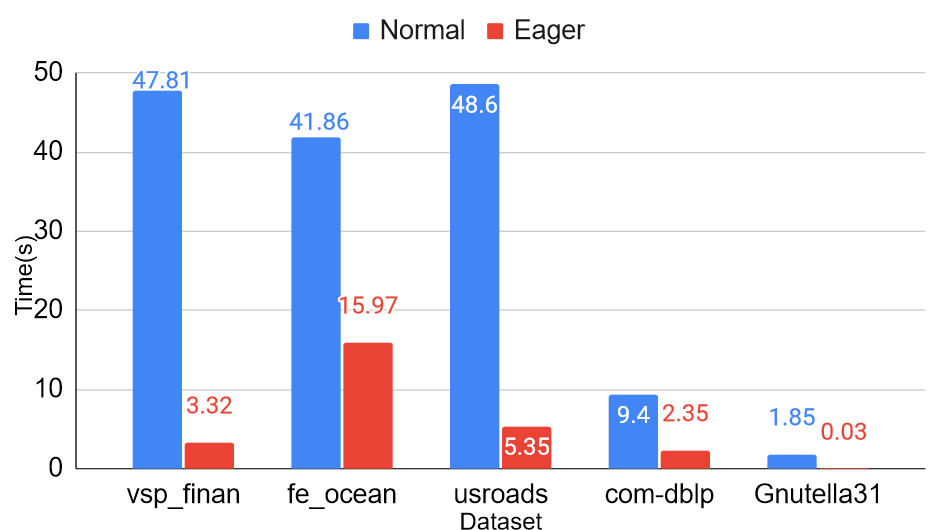
\includegraphics[width=0.93\linewidth]{figures/compare_buffer.png}
%     \caption{\fontsize{9}{11}\selectfont Buffer allocation time with/without eager buffer management of \tool{} on NVIDIA H100. (Normal is EBM disabled, Eager is EBM enabled)}
%     \label{fig:buffer_compare}
%     % \vspace{-0.4cm}
% \end{figure}

% \begin{figure}[h]
%     \centering
%     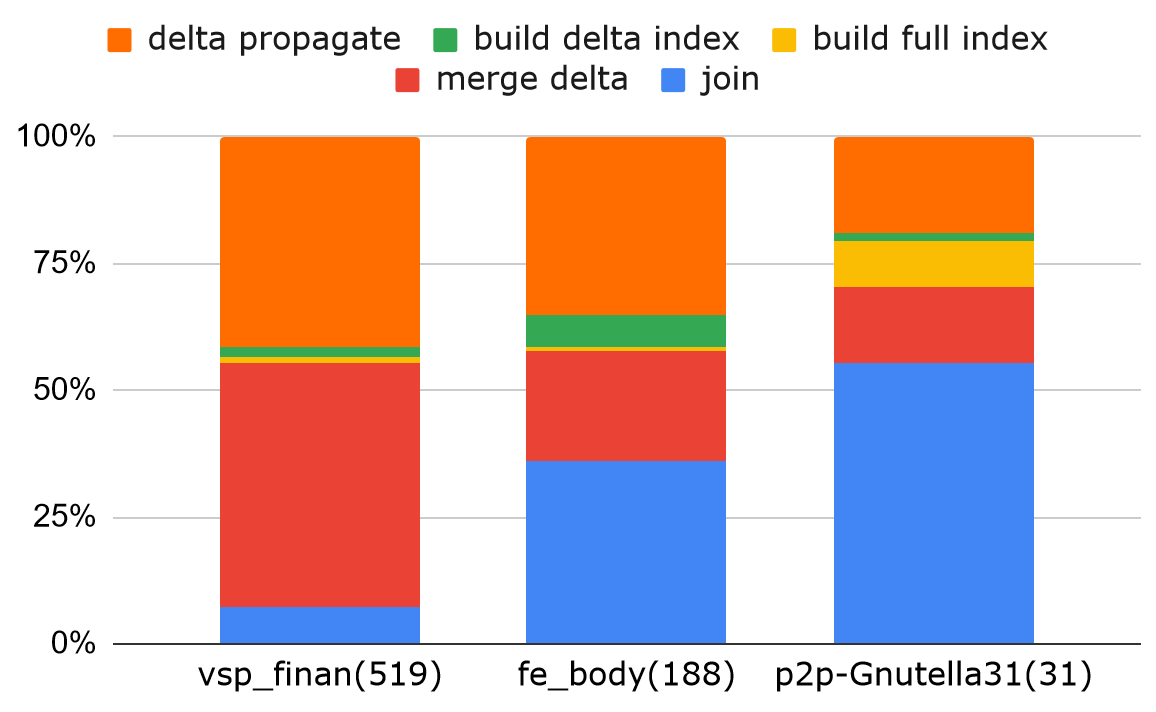
\includegraphics[width=\linewidth]{figures/tc_detail_ratio.png}
%     \caption{Running time analysis of Reachability query in \tool{} with different number of iterations, when \buffer is disabled.}
%     \label{fig:tc_iter_compare}
% \end{figure}


% \subsection{Evaluating k-way Join Performance}


% \begin{table}[]
%     \begin{tabular}{@{}ccccc@{}}
%     \toprule
%     Dataset & Average& Number& Join Rate & Build Rate \\
%     name&values/key&of edges& \multicolumn{2}{c}{(Billions of tuples/sec)} \\
%     \midrule
%     com-dblp   & 6.62          & 1.05M & 0.51   & 0.90       \\
%     vsp-finan  & 7.89          & 552k   & 0.67   & 0.77       \\
%     fc-ocean   & 5.71          & 410k    & 0.61   & 0.74       \\
%     CA-Hepth   & 5.26          & 51.9k    & 0.39   & 0.17       \\
%     fe\_sphere & 5.99          & 49.2k    & 0.20   & 0.34       \\           
%     \bottomrule
%     \end{tabular}

%     \caption{\tool{} hash table performance test.}
% \end{table}

\begin{table}[h]
    \fontsize{9}{11}\selectfont
    \caption{\fontsize{9}{11}\selectfont Reachability execution time comparison: \tool{} (NVIDIA H100) vs. Souffl\'e (AMD Milan CPU 32 cores), GPUJoin, and cuDF on large graphs (OOM: out of memory).}  
    \begin{tabular}{c||c||c|c|c|c}
    \toprule
    \multicolumn{1}{c}{Dataset} & \multicolumn{1}{c}{\textit{Reach}} & \multicolumn{4}{c}{Time (s)} \\ 
    \multicolumn{1}{c}{name} & \multicolumn{1}{c}{edges} & \tool{}      & Souffl\'e     & GPUJoin  & cuDF  \\ \midrule
    com-dblp            & 1.91B    & \textbf{14.30}     & 232.99   &  OOM    & OOM \\
    fe\_ocean           & 1.67B    & \textbf{23.36}     & 292.15   &  100.30 & OOM \\
    vsp\_finan          & 910M      & \textbf{21.91}     & 239.33   &  125.94 & OOM \\
    Gnutella31          & 884M      & \textbf{5.58}      & 96.82    &  OOM    & OOM \\ 
    fe\_body            & 156M      & \textbf{3.76}      & 23.40    &  22.35  & OOM \\
    SF.cedge            & 80M       & \textbf{1.63}      & 33.27    &  3.76  & 64.29 \\ 
    \bottomrule
    \end{tabular}
   \label{tab:reach_compare}
\end{table}


\subsection{\tool{} vs. SOTA GPU joins}

\label{eval:vs-other-joins}

In this section, we evaluate the performance of the \textit{REACH} query using \tool{}, GPUJoin, and cuDF, with Souffl\'e serving as the baseline. The results are summarized in Table~\ref{tab:reach_compare}.
The datasets used in the experiments represent a diverse array of sources, ensuring a comprehensive assessment that spans scientific communities, P2P networks, random graphs, and road networks. This dataset diversity helps mitigate any bias towards specific graph categories. 



\begin{table}[t]
    \fontsize{9}{11}\selectfont
    \caption{\fontsize{9}{11}\selectfont Same Generation (\emph{SG}) execution time comparison: \tool{} vs. Souffl\'e  and cuDF. Souffl\'e running \revised{32 core AMD Milan CPU}; \tool{} and cuDF running on NVIDIA H100 GPU.}   
    % \begin{tabular}{lllll}
    \begin{tabular}{c||c||c|c|c|c}
    \toprule
    \multicolumn{1}{c}{\multirow{2}{*}{Dataset}} & \multicolumn{1}{c}{\multirow{2}{*}{SG size}} & \multicolumn{3}{c}{Time (s)} \\ 
    \multicolumn{1}{c}{}                         & \multicolumn{1}{c}{}                         & \tool{} & HIP      & Souffl\'e     & cuDF    \\ \midrule
    fe\_body                                     & 408M                                  & \textbf{5.05} & 19.57     & 74.26       & OOM    \\
    loc-Brightkite                               & 92.3M                                  & \textbf{3.42} & 14.00      & 48.18       & OOM        \\
    fe\_sphere                                   & 205M                                  & \textbf{2.36} & 8.48      & 48.12       & OOM        \\
    SF.cedges                                     & 382M                                   & \textbf{5.54} & 20.57      & 68.88       & OOM        \\
    CA-HepTH                                     & 74M                                   & \textbf{2.79} & 5.92      & 20.12       & 21.24        \\
    % delaunay\_n16 & 26M & \textbf{0.89} & 6.68  & 14.83 \\
    ego-Facebook  & 15M & \textbf{1.23} & 2.81 & 17.01 & 19.07 \\
    \bottomrule
    \end{tabular}
   \label{tab:sg_compare}
\end{table}

\tool{} consistently emerges as the fastest engine in all test cases. Compared to GPUJoin, \tool{} exhibits a remarkable speedup, with ratios often exceeding 3x. In the  ``fe\_body'' testcase, the speedup ratio reaches an impressive 6x. Notably, GPUJoin, designed specifically for reachability queries, stores output relations in raw arrays. This specialization suggests that \tool{} could achieve even higher speedup ratios when the method of GPUJoin is applied to general  queries.
Compared to GPUJoin, \tool{} used less memory: GPUJoin OOM'd twice during testing. This is because of its of use open-addressing-based hashmaps for storing relations, necessitating a low hashtable loading factor to facilitate joins.  By contrast, HISA employs hash tables only for accelerating range fetching on indexed relations. This results in efficient access even with a higher load factor ($0.8$).

%In contrast with \tool{}, cuDF's implementation yields unsatisfactory results, even when compared to the baseline CPU-based approach. It's complex code base makes it challenging to perform a detailed memory profile, but the presence of numerous out-of-memory errors during experiments points to memory-related performance issues. High memory usage significantly affects memory allocation and deallocation for buffer and tuple storage, contributing to slow running times.


\begin{figure*}[t]
\begin{tabular}{ccc}
\begin{minipage}{.46\textwidth}
    \captionof{table}{\fontsize{9}{11}\selectfont Context-Sensitive Program Analysis \emph{(CSPA)} execution time comparison: \tool{} (NVIDIA H100) vs. Souffl\'e (\revised{32 core AMD Milan CPU}); input data from~\cite{awad2019engineering}.}
    \label{tab:cspa_compare} 
\resizebox{\textwidth}{!}{\begin{tabular}{@{}c||c|c||cc||c@{}}
    \toprule
    Dataset    & Input Relation  & Output Relation  & \multicolumn{2}{c}{Time (s)}    & Speedup \\
    Name       & Size            & Size             & \tool{} & Souffl\'e              &      \\ \midrule
    Httpd      & \begin{tabular}[c]{@{}c@{}}Assign: 3.62e5\\ Dereference: 1.14e6\end{tabular} & \begin{tabular}[c]{@{}c@{}}ValueFlow: 1.36e6\\ ValueAlias: 2.34e8\\ MemAlias:8.89e7\end{tabular} &\textbf{1.33}         & 49.48   & \textbf{37.2x}   \\ \midrule
    Linux      & \begin{tabular}[c]{@{}c@{}}Assign: 1.98e6\\ Dereference: 7.50e6\end{tabular} & \begin{tabular}[c]{@{}c@{}}ValueFlow: 5.50e6\\ ValueAlias: 2.23e7\\ MemAlias:8.84e7\end{tabular} & \textbf{0.39}        & 13.44   & \textbf{34.5x}    \\ \midrule
    PostgreSQL & \begin{tabular}[c]{@{}c@{}}Assign: 1.20e6\\ Dereference: 3.46e6\end{tabular} & \begin{tabular}[c]{@{}c@{}}ValueFlow: 3.71e6\\ ValueAlias: 2.23e8\\ MemAlias:8.84e7\end{tabular} & \textbf{1.27}       & 57.82   & \textbf{44.9x}   \\
    \bottomrule
    \end{tabular}}
\end{minipage}
& 
\begin{minipage}{0.02\textwidth} % This is the spacer minipage
\hfill % Optional: use \hfill to adjust spacing further
\end{minipage}
&  
\begin{minipage}{.46\textwidth}
    \centering
    % 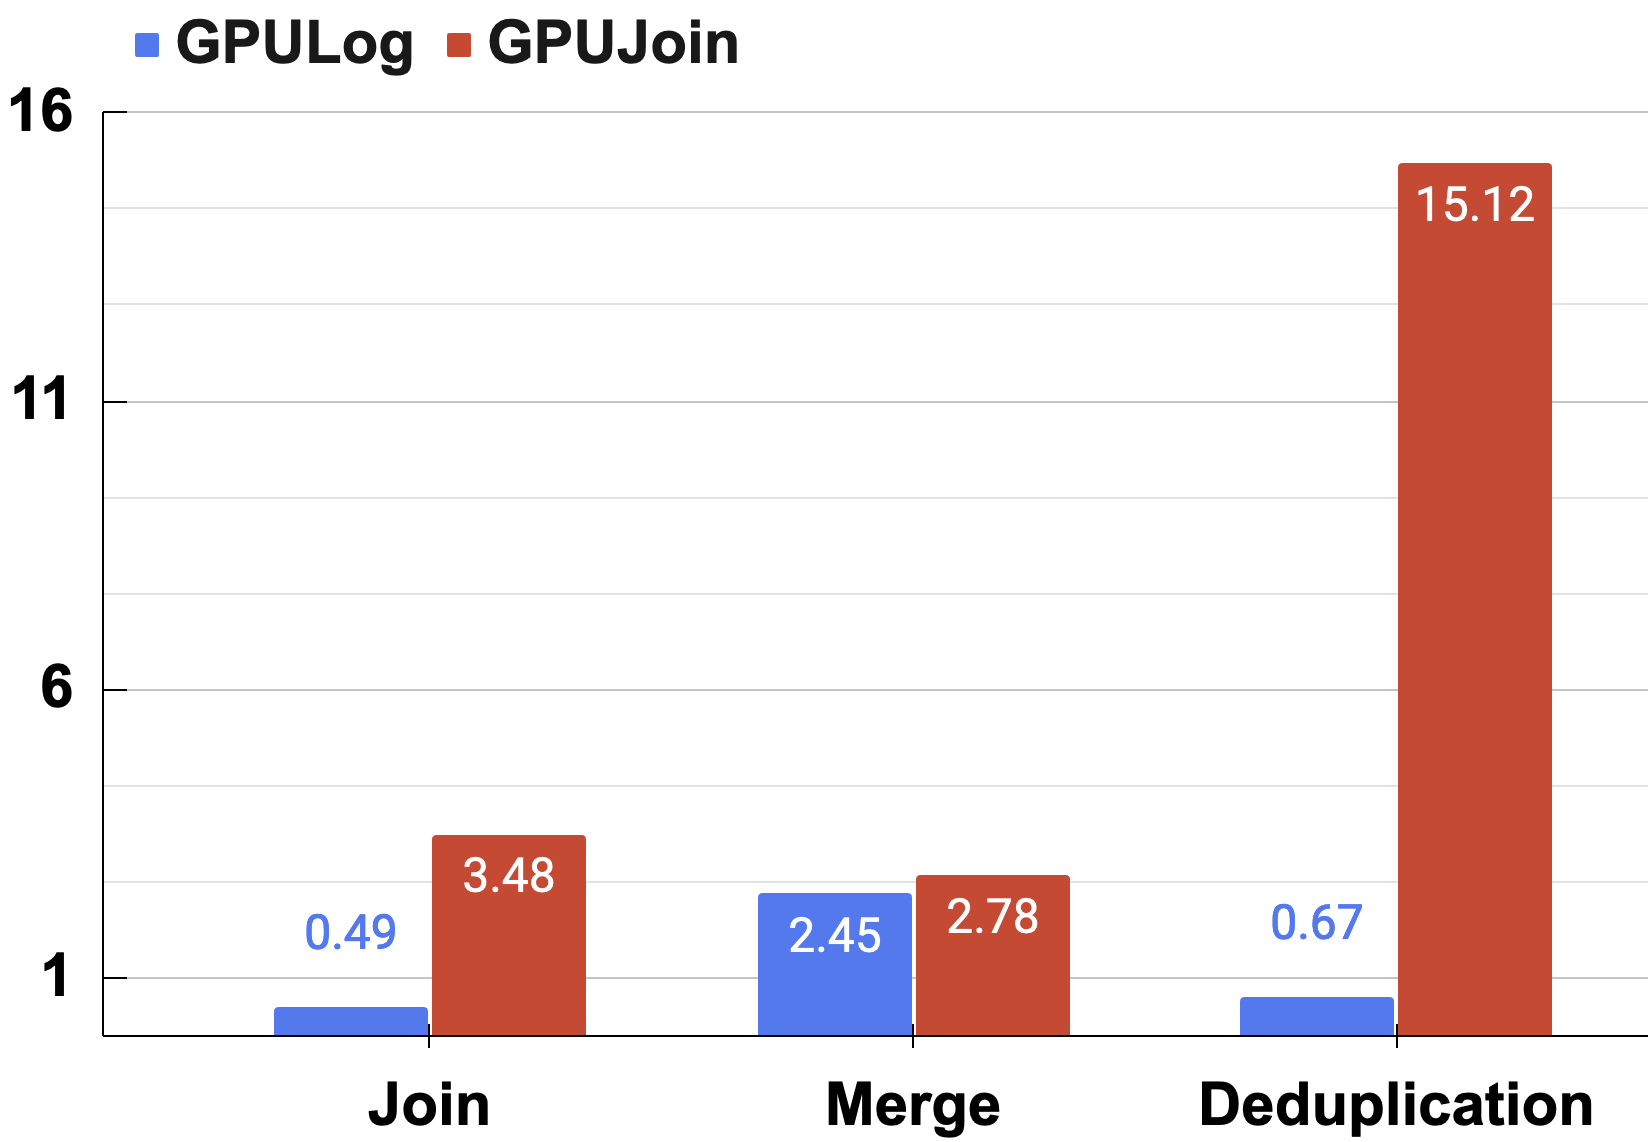
\includegraphics[width=\linewidth]{figures/detail_compare.png}
    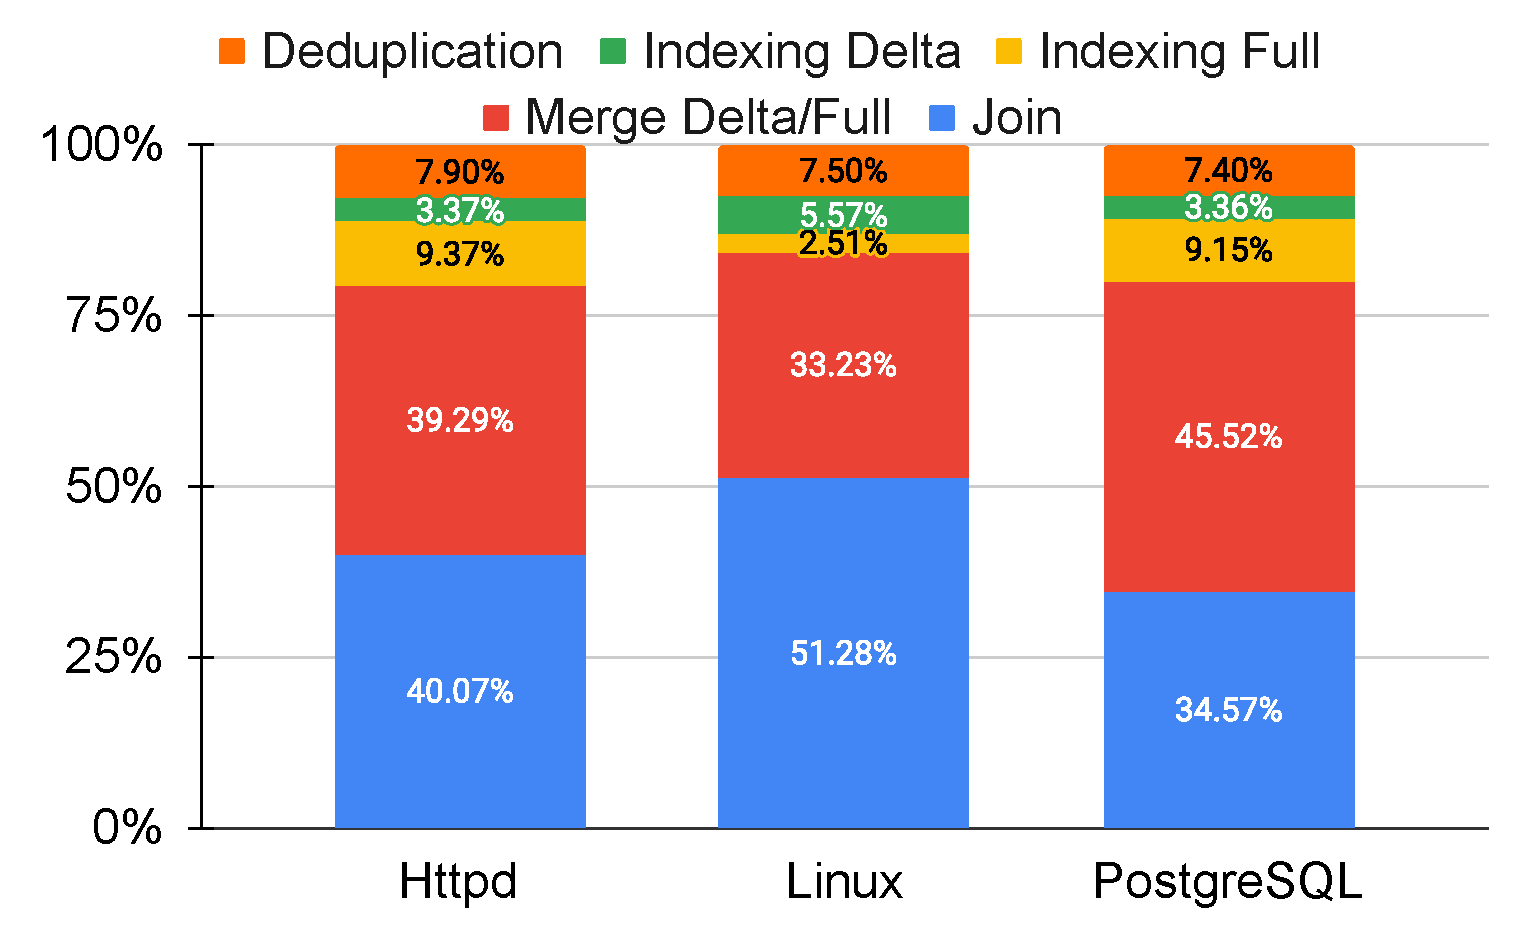
\includegraphics[width=\linewidth]{figures/cspa_detail.pdf}
    \caption{\fontsize{9}{11}\selectfont Running time detail analysis of \textit{CSPA} query using \tool{} on various real world datasets on NVIDIA A100.}
    % \caption{\revised{\fontsize{9}{11}\selectfont Running time detail of \textit{REACH} query using \tool{} and GPUJoin on fe\_body datasets on NVIDIA H100.}}
    \label{fig:join_detail}
\end{minipage}
\end{tabular}
\end{figure*}

We present another test case, \textit{SG}, to further validate our previous discussions. The results are presented in Table~\ref{tab:sg_compare}. The \textit{SG} query involves $n$-way joins and represents more general use cases. As GPUJoin does not support the SG query, we exclusively compare \tool{} with cuDF. Across all six test cases, cuDF encounters out-of-memory (OOM) errors four times, while the non-OOM test cases, although approaching the baseline performance of Souffl\'e, remain considerably slower than \tool{}. \tool{} consistently delivers stable performance, running nearly 7$\times$ faster than the baseline in most of cases, while not experiencing any OOM error. 

% \revised{To better understand how the system design differences between \tool{} and GPUJoin impact runtime, we measured the most time-consuming components of both engines, as shown in Figure~\ref{fig:join_detail}. In the figure, ``Join'' represents the time spent on performing the join operation and materializing the results in both tools. In \tool{}, ``Merge'' refers to the time required to merge the delta tuples into the full, while ``Deduplication'' represents the time taken to remove duplicate tuples during iterative computation.
% The results show that \tool{} has a faster join speed compared to GPUJoin, due to the more efficient join algorithm and the fast range queries discussed in the second paragraph of Section~\ref{sec:join-impl}. The merge phase running time for both tools is similar, although merging the more complex HISA data structure in \tool{} takes more time, GPUJoin’s fused delta population and merge process (as discussed in the third paragraph pf Section~\ref{sect:pop-delta}) results in merging undeduplicated tuples, which increases both the number of tuples and the time required for merging.
% This fused design in GPUJoin causes deduplication to become a bottleneck, as it requires scanning the entire full relation to remove duplicates—an expensive operation when the tuple size is large. In contrast, \tool{}’s effective iterative evaluation design ensures that the deduplication time remains reasonable.}

\subsection{Context-Sensitive Program Analysis}
% comparing CSPA with souffle

Program analysis is one of the most popular applications of Datalog, with several state-of-the-art tools (DOOP~\cite{bravenboer2009doop}, cclyzer~\cite{balatsouras2016cclyzer}, and ddisasm~\cite{flores2020ddisasm}) implemented using Souffl\'e Datalog. To evaluate \tool{}'s potential application to program analysis, we implemented context-sensitive points-to analysis (\textit{CSPA}), reproducing the experiments of Graspan~\cite{Wang2017GraspanAS}. We elide the full query for space, it includes rules which initialize and propagate value flows, while simultaneously discovering alias information; Graspan uses method cloning (effecting inling) for context sensitivity.
%
% The \textit{CSPA} query, illustrated in Figure~\ref{fig:cspa-code}, includes two EDB relations: \textit{assign}, recording static variable assignments in the target program, and \textit{deref}, tracking pointer dereferences; these relations are constructed by a preprocessing pass. The rules of the query forms an Andersen-style data flow analysis, encapsulated the results in the IDB relation \textit{ValueFlow}, which delineates possible values of variables within specific calling contexts (encoded in the data via method cloning). The other two IDB relations, \textit{MemAlias} and \textit{ValueAlias}, record value and memory equivalences, respectively. The bottom five rules are used to initialize values in IDB relations; the mutually-recursive five upper rules declare the tuple population in the IDB rules. For instance, the first rule establishes the transitive nature of \textit{ValueFlow}, while the second rule addresses the scenario where two values, flowing to the identical variable under the same context, are deemed equivalent (a situation indicative of value flow conflation and precision loss in context-sensitive point-to analysis).
%
%
Using Graspan's data, we ran \textit{CSPA} on \textsf{httpd}, 
(a statically-linked subset of) \textsf{linux}, and \textsf{postgres}~\cite{Wang2017GraspanAS}. The results of our evaluation are presented in Table~\ref{tab:cspa_compare}; the table lists the size of input and output relations (second and third columns) and total running time (fourth column). All relation sizes match that of Souff\'e's.
% The large tuple sizes in both input and output make the query highly data-intensive, representing an attractive candidate for SIMD-based parallelization.

\yihao{We see a roughly 35-45$\times$ speedup versus Souffl\'e under ideal conditions (Souffl\'e use $32$ cores CPU with all optimizations, \tool{} running on NVIDIA H100 with maximum buffer size), demonstrating the significant performance advantage of \tool{} over the CPU-based Souffl\'e. This is mainly because the memory-heavy nature of program analysis workloads. Memory bandwidth and throughput significantly affect performance, and CPU systems usually have lower memory bandwidth. For example, the AMD Milan's bandwidth is around 190 GB/s, while a data center GPU like the NVIDIA H100 can have up to 3.35 TB/s. The lower memory speed and throughput prevent CPU-based systems from fully utilizing their high single-core performance. Our detailed analysis on CPU utilization further proves this, despite utilizing all 32 CPU cores during computation, the efficiency of Souffl\'e was relatively low, with CPU ratios of 571\%, 449\%, and 683\% for the \textsf{httpd}, \textsf{Linux}, and \textsf{PostgreSQL} datasets, respectively. Note that a 100\% utilization across 32 cores should yield a CPU ratio of 3200\%. }

Figure \ref{fig:join_detail} breaks down different phases of \tool{} when running our queries. In this figure, ``Deduplication'' shows time spent coalescing previously-discovered facts. ``Indexing Full/Delta'' represents the time required for creating hash indexing within \tool's hybrid data structure. `
`Merge Delta/Full'' captures the time spent on inserting all tuples from the delta relation into the full relation using GPU merge. 
Finally, ``Join'' represents the actual time spent performing join operations across all relations. 
\revised{The join (39\% of total runtime) and merge (42\% of total runtime) operations stand out as the most time-consuming phases in our pipeline, as depicted in the red and blue bar in the Figure~\ref{fig:join_detail}. Since performing joins between relations is computationally intensive and one of our main focuses, we expect this phase to occupy a significant portion of the total runtime. By leveraging the HISA datastructure, \tool{} is able to make these joins more efficient than previous GPU-based systems~\cite{shovon2023towards,shovon2022accelerating}. However, as the figure indicates, the merge operation is even more time-consuming than the join phase. 
This is due to the reason that lock-free style parallel path merge aglorithm we used require pre-allocating a result buffer that matches the combined size as total size of delta and full. Since the full relation in Datalog is typically large, this result buffer can be substantial. Allocating and freeing such a large buffer in every iteration is expensive, and, according to our detailed timing results, this step becomes even more time-consuming than the join and indexing operations in the query.
To partially address this challenge, we introduce an amortized buffer management scheme (described in Section~\ref{sec:impl-buffer}). While this approach doesn’t fully resolve the issue, it mitigates the need to allocate buffers at every iteration, thereby reducing the overall computational load.}
% The bottleneck for \textit{CSPA} lies in both merge and join. These phases are both highly data-intensive components which are significantly accelerated by leveraging GPU-based parallel sort and merge algorithms. Our results demonstrate the potential of GPU-based tools for data-intensive program analysis.


% \begin{figure}
%     \centering
%     $\begin{array}{rcl}
%         \textit{ValueFlow}(x, y) & \leftarrow & \textit{ValueFlow}(x, z), \textit{ValueFlow}(z, y). \\
%         \textit{ValueAlias}(x, y) & \leftarrow & \textit{ValueFlow}(z, x), \textit{ValueFlow}(z, y). \\
%         \textit{ValueFlow}(x, y) & \leftarrow & \textit{assign}(x, z), \textit{MemAlias}(z, y). \\
%         \textit{MemAlias}(x, w) & \leftarrow & \textit{deref}(y, x), \textit{ValueAlias}(y, z), \\ 
%                                    &            & \textit{deref}(z, w). \\
%         \textit{ValueAlias}(x, y)  & \leftarrow & \textit{ValueFlow}(z, x), \textit{MemAlias}(z, w), \\
%                                    &            & \textit{ValueFlow}(w, y). \\
%         \textit{ValueFlow}(y, x) & \leftarrow & \textit{assign}(y, x). \\
%         \textit{ValueFlow}(x, x) & \leftarrow & \textit{assign}(x, y). \\
%         \textit{ValueFlow}(x, x) & \leftarrow & \textit{assign}(y, x). \\
%         \textit{MemAlias}(x, x) & \leftarrow & \textit{assign}(y, x). \\
%         \textit{MemAlias}(x, x) & \leftarrow & \textit{assign}(x, y).
%     \end{array}$
%     \caption{Datalog code for Context-Sensitive Program Analysis (\textit{CSPA}). \textit{assign} and \textit{deref} constitute EDB relations.}    \label{fig:cspa-code}
% \end{figure}

%Figure \ref{fig:cspa_join_detail} shows relative running time across different phases of \tool{}'s execution. 


% A detailed examination of the CPU utilization ratio of Souffl\'e revealed that, despite utilizing all $32$ CPU cores during computation, the efficiency of Souffl\'e was relatively low, with CPU ratios of $571$\%, $449$\%, and $683$\% for the \textsf{}httpd, \textsf{Linux}, and \textsf{PostgreSQL} datasets, respectively. Note, a $100$\% utilization across $32$ cores should yield a CPU ratio of $3200$\%. 
% This discrepancy is primarily due to the MIMD nature of multi-core-based engines, which struggle to effectively parallelize program-analysis queries with large volumes of data. 

\subsection{\tool{} Across Different Hardware}
\label{sec:protablility}
To increase the performance portability of \tool{}, we translated it to a Heterogeneous-Compute Interface for Portability (HIP)~\cite{AMD_2024} based engine (\tool{}-HIP hereafter) with an identical API to our vanilla CUDA variant. This interface enables seamlessly switching \tool{} implementations from NVIDIA to HIP kernels. %In both CUDA and HIP, memory allocation plays a crucial role in enabling efficient parallel processing on GPUs. CUDA, developed by NVIDIA, and HIP, an open-source alternative primarily supported by AMD, share similarities in their approach to memory management but also exhibit notable differences. CUDA utilizes a specific set of memory allocation functions to allocate and deallocate memory on the GPU device, enabling data transfers between the CPU and GPU. CUDA's memory allocation is tightly integrated with its programming model, offering developers a streamlined experience when working with NVIDIA GPUs.
 The HIP version of \tool{}, while not matching the CUDA version's performance (due to missing libraries such as RMM \cite{librmm}), offers broad compatibility with different GPU architectures. This enables rapid deployment on the exascale systems, for example, Frontier and Aurora \cite{alcf-aurora,frontier}, which do not support CUDA.

\begin{table}[]
\fontsize{9}{11}\selectfont
\caption{\fontsize{9}{11}\selectfont Comparison of \tool{} and \tool{}-HIP running times across various GPU vendors and models } 
\begin{tabular}{@{}c|c|c|c||c|c@{}}
 % \multicolumn{2}{c}{}         & \multicolumn{4}{c}{Time (s)} \\
%\toprule
 \multicolumn{2}{c}{}          & \multicolumn{2}{c||}{\tool{} (NVIDIA)}    & \multicolumn{2}{c}{\tool{} (AMD)}      \\ 
%\midrule
 Query            & Dataset               & H100     & A100    & MI250    & MI50      \\ 
 \midrule
             & fe\_body       & 5.05     & 8.61    & 19.57    & 41.99     \\
SG           & BrightKite & 3.42     & 6.79    & 14.00    & 30.05     \\
             & fe\_sphere     & 2.36     & 4.64    & 8.48     & 19.426    \\ \midrule
             & \textsf{httpd}          & 1.33     & 2.73    & 6.75     & 15.27         \\
CSPA         & \textsf{linux}          & 0.39     & 0.77    & 1.39     & 3.32         \\
             & \textsf{postgres}     & 1.27     & 2.68    & 6.79     & 14.55         \\ \bottomrule
\end{tabular}
\label{tab:different-gpu}
\end{table}

To compare \tool{}'s performance across a range of data center GPUs, we ran \textit{SG} and \textit{CSPA} using \tool{} on the NVIDIA H100 and A100 and the AMD MI250 and MI50. The outcomes of these tests are presented in Table~\ref{tab:different-gpu}. The NVIDIA H100, successor to the A100, features more SM units ($114$ vs. $108$), double the FP32 cores per SM ($128$ vs. $64$), and improved memory bandwidth (2TB/s vs. 1.5TB/s). Columns 4 and 5 of our results show \tool{} benefits from these enhancements. % In every test, the H100 consistently delivers performance that is approximately twice as fast as the A100. Our results illustrate that \tool{} effectively harnesses the additional throughput offered by the latest GPUs.

The last two columns illustrate \tool{}'s performance on AMD GPUs. The MI250, with 104 computational units ($64$ core per unit) akin to NVIDIA’s SMs, shows comparable performance to the NVIDIA A100 in \textit{CSPA} tests but lags in \textit{SG} tests requiring more memory, performing at about half the A100's speed. The MI50, with half the capacity of the MI250, displays nearly half its performance, pointing towards the scalability of the approach. MI250 has similar total computational resources, it should have similar performance to the A100. However, the most important reason for the lower performance of the AMD MI250 is its dual chiplet design; since \tool{} is a single-GPU system, only half of the compute resources on the MI250 can be utilized, resulting in half the performance of the A100. Another reason is our use of the NVIDIA-specific RMM library in our implementation. Since AMD's ROCm does not support this library, we rely on manual memory pooling instead; we leave optimizing memory allocation in our HIP backend to future work.
 %In conclusion, our experiments demonstrate the robustness and scalability of \tool{} across diverse GPU architectures, including its capability to leverage advancements in GPU technology,


\begin{table}[]
    \centering
    \fontsize{9}{11}\selectfont
    \caption{\fontsize{9}{11}\selectfont Comparing Time Consuming Operation of \tool{} on AMD EPYC 7543P 32-core Zen 3 CPU and NVIDIA A100 GPU. Each running time in table are in seconds.}
    \label{tab:gdlog-cpu}
    \begin{tabular}{c|c c|c c|c c}
    \toprule
    & \multicolumn{2}{c}{Sort} & \multicolumn{2}{c}{Merge} & \multicolumn{2}{c}{Memory} \\
    \# Tuples  & \textbf{A100} & \textbf{Zen3} & \textbf{A100} & \textbf{Zen3} & \textbf{A100} & \textbf{Zen3} \\
    \hline
    1,000,000 & 0.12 & 1.09 & 0.03 & 0.06 & 0.03 & 0.02 \\
    10,000,000 & 0.39 & 7.5 & 0.08 & 0.64 & 0.17 & 0.05 \\
    50,000,000 & 1.63 & 30.09 & 0.18 & 1.96 & 0.11 & 0.88 \\
    100,000,000 & 2.9 & 64.02 & 0.3 & 3.56 & 0.18 & 1.7 \\
    500,000,000 & 15.66 & 351.4 & 1.21 & 15.68 & 0.82 & 8.59 \\
    \bottomrule
    \end{tabular}
\end{table}

Although fully implementing \tool{} on a CPU via SIMD is possible, we believe such an implementation would not achieve similar performance due to the significant memory bandwidth differences between the two hardware architectures. Due to the extensive potential engineering work, we did not implement a full CPU version of \tool{}. However, we did implement two \tool{}'s most computationally-expensive phases: sort, merge and implemented them using the latest version of Intel's oneTBB SIMD library (which uses CPU-specific vectorization)~\cite{onetbb}.

We ran both CPU and GPU implementations of sort and merge on different sizes of randomly generated tuples with two arities, collecting the total time of 100 runs. The results are presented in Table~\ref{tab:gdlog-cpu}. Overall, in all test cases, the GPU version of both sort and merge functions is around 10x to 20x faster than the CPU version. We believe this is primarily due to the significantly better memory bandwitdh offered by the GPU (1.5 TB/s vs. 0.19 TB/s). To investigate this, we collected the buffer allocation and initialization times for these two operations and listed them in the last column, which shows the memory allocation and initialization of the buffer to hold tuples used in the experiment. For all input sizes, the A100 GPU is consistently 10x faster than the EPYC 7543. We note that the performance increases mirror the memory bandwidth differences between the CPU and GPU; indeed, because modern Datalog applications (such as \textit{CSPA}) are memory-bound, we conclude GPUs offer an attractive implementation platform for modern Datalog engines.
 


\section{Conclusion and Future Work}

%Modern in-memory Datalog engines typically hit scalability walls around $8$--$16$ threads, due to limited memory bandwidth and the overhead of locking. The extreme parallel throughput offered by modern GPUs make them an attractive candidate for the implementation of high-performance backends for Datalog that modern power program analyses and similar applications. However, current approaches to GPU Datalog are stymied by incomplete implementations, limited expressivity, and a lack of data structures specialized to the concerns of modern Datalog evaluation (iterated joins and semi-na\"ive evaluation). 

We presented \tool{}, the first GPU-based Datalog engine able to achieve net-positive performance compared to SOTA Datalog implementations. Our library \tool{} (implemented both for CUDA and HIP) enables modern Datalog implementation techniques, namely compilation to relational algebra, range-indexed iterated joins, and optimized $n$-way joins. \tool{} is powered by the hash-indexed sorted array (HISA), a novel data structure we developed to support high-performance Datalog engines on the GPU. 
%HISA combines the algorithmic necessities of modern Datalogs while effectively leveraging the massive SIMD parallelism available to modern GPUs. 
We then used HISA to build \tool{} by employing two novel design points: temporarily materialized $n$-way joins and eager buffer management. We have evaluated \tool{} extensively compared to both CPU and GPU-based state-of-the-art; our experimental results demonstrate improvements of up to $45\times$ compared to an optimally-tuned CPU-based engine on context-sensitive points-to analysis of \textsf{PostgreSQL}.

% We plan several threads of future work. 
\revised{We notice recent work on running relational algebra and Datalog on multi-node systems, scaling them to thousands of nodes~\cite{sun2023communication, gilray2021compiling, kumar2020load, kumar2019distributed} using fine-tuned MPI all-to-all communication~\cite{fan2024configurable, fan2022optimizing}.
Following this trend, one of our future projects is multi-node, multi-GPU programming coordinated via MPI. Such an effort necessitates a heterogeneous decomposition of work across nodes while minimizing communication. We plan to address this by leveraging the coarse-grained (task-level) parallelism inherent in specific applications.} Additionally, we intend to extend \tool{} to support monotonic aggregation and implement recent join algorithms, such as free join~\cite{freejoin}.

%We believe our work shows the potential for GPUs to bring orders-of-magnitude performance improvements to analytics applications in program analysis, graph mining, medical reasoning, and similar deduction-heavy domains; we are currently applying \tool{} to large applications in several of these areas. As future work, we hope to explore multi-GPU joins, especially in the context of modern GPU interconnects and heterogeneous communication. We also hope to extend \tool{} to enable incremental computations over large data streams on modern data center GPUs.

\section{Acknowledgement}
This work was funded in part by NSF RII Track-4 award 2132013, NSF PPoSS planning award 2217036, NSF PPoSS large award 2316157 and, NSF collaborative research award 2221811. We are thankful to the ALCF’s Director’s Discretionary (DD) program for providing us with compute hours to run our experiments on the Polaris supercomputer and the Joint Laboratory for System Evaluation (JLSE) located at the Argonne National Laboratory. 
% This material is based upon work supported by the Defense Advanced Research Projects Agency (DARPA) under Contract No. N66001-21-C-4023. Any opinions, findings and conclusions or recommendations expressed in this material are those of the author(s) and do not necessarily reflect the views of DARPA.

\bibliographystyle{plain}
\bibliography{main}

\end{document}

